\documentclass[12pt,a4paper,twoside,openright]{report}

\usepackage{afterpage}


% --- 1. CONFIGURACIÓN BÁSICA Y FUENTES ---
\usepackage[utf8]{inputenc}
\usepackage[T1]{fontenc}   
%\usepackage{lmodern}          % Fuentes nítidas y completas
\usepackage{microtype}        % Evita que el texto se salga de los márgenes

%times en texto y default de latex en formulas
\renewcommand{\rmdefault}{ptm}



% Márgenes para encuadernación (A4)
\usepackage{geometry}
\geometry{
    a4paper,
    left=30mm,   
    right=30mm,
    top=25mm,
    bottom=25mm
}

\usepackage{setspace}
\singlespacing % interlineado sencillo
%\onehalfspacing %interlineado 1.5

% --- 2. PAQUETES DE FÍSICA Y MATEMÁTICA (CRÍTICO) ---
\usepackage{amsmath}     % Ecuaciones avanzadas
\usepackage{amssymb}     % Símbolos matemáticos extra
%\usepackage{siunitx}     % INDISPENSABLE para Física Experimental
                         % Uso: \qty{9.8}{m/s^2} o \num{3.4+-0.1}
\usepackage{physics}
\usepackage{bm}
\usepackage{bbm}
\usepackage{enumitem}
\usepackage{mathtools}

% --- 3. GRÁFICOS Y TABLAS ---
\usepackage{graphicx}
\usepackage{float}       % Para usar [H] y clavar las figuras donde quieras
\usepackage{caption}
\usepackage{subcaption}  % Para poner fig (a) y (b) lado a lado
\usepackage{booktabs}    % Tablas profesionales (usa \toprule, \midrule, \bottomrule)
\usepackage[table]{xcolor} 
\usepackage{adjustbox}
% Permite superponer texto (porcentual) sobre imágenes: \begin{overpic}[width=..]{...}\put(x,y){...}
\usepackage[percent]{overpic}
\renewcommand{\tablename}{Tabla}
\AtBeginDocument{\renewcommand{\tablename}{Tabla}}

% --- 3.1 PRESENTACIÓN DE SCRIPTS ---

\usepackage{minted}
%\captionsetup{font=small}
\captionsetup{font={footnotesize,stretch=1}}

% --- 4. IDIOMA Y REFERENCIAS ---
\usepackage[english,main=spanish]{babel}
\usepackage[english]{babelbib}           
\usepackage{hyperref}
\hypersetup{
    colorlinks=true,       
    allcolors=black,       % Negro para imprimir
    linktoc=all
}

% --- 5. FORMATO DE TÍTULOS ---
\usepackage{titlesec}

%Creative Commons
\usepackage[
    type={CC},
    modifier={by-nc-sa},
    version={4.0},
]{doclicense}

% Esto configura el estilo para que diga "Capítulo N" arriba y el título abajo
\titleformat{\chapter}[display]
  {\normalfont\huge\bfseries} % Estilo del texto
  {\chaptertitlename\ \thechapter} % "Capítulo 1"
  {20pt} % Espacio entre "Capítulo 1" y "RMN"
  {\Huge} % Tamaño del título del capítulo

\usepackage{emptypage}


\begin{document}

\begin{titlepage}

    \noindent % Evita la sangría por defecto
    \begin{minipage}[c]{0.45\textwidth}
        % Logo izquierdo (UNC)
        
\includegraphics[width=4.5cm]{images/logo_unc.jpg} 
    \end{minipage}%
    \hfill % Este comando empuja los bloques a los extremos
    \begin{minipage}[c]{0.45\textwidth}
        \begin{flushright}
            % Logo derecho (FAMAF)
            
\includegraphics[width=6cm]{images/logo_famaf.png} 
        \end{flushright}
    \end{minipage}

\begin{center}

\LARGE
\textbf{Parametrización geométrica y resolución espacial de un microtomógrafo de rayos X de arquitectura abierta}

\vspace{1cm}

por

\vspace{0.3cm}

\textbf{Mateo José Sironi Nuñez}

\vspace{1cm}





\Large
Presentado ante la FACULTAD DE MATEMÁTICA, ASTRONOMÍA, FÍSICA Y COMPUTACIÓN
como parte de los requerimientos para la obtención del grado de 
Licenciado en Física de la

\vspace{0.6cm}

UNIVERSIDAD NACIONAL DE CÓRDOBA

\vspace{0.6cm}

Mayo, 2026

\vspace{1cm}

\textbf{Director}: Dr. Germán Tirao\\

\vspace{1cm}

\normalsize
\doclicenseThis


\end{center}
\end{titlepage}
\afterpage{\null\thispagestyle{empty}\newpage}
\setcounter{page}{1}
\chapter*{Resumen}

Este trabajo describe el desarrollo e implementación de un protocolo integral de
calibración y optimización para un sistema de microtomografía computarizada de rayos X ($\mu$CT)
de arquitectura abierta. El objetivo central fue transformar un conjunto de componentes
independientes en un instrumento de alta precisión para la investigación científica,
comparable a un dispositivo comercial.

La metodología comenzó con la estabilización del hardware, fijando la fuente y el
detector sobre una base rígida para eliminar desalineaciones accidentales. Se
implementaron técnicas de alineación física mediante el análisis de proyecciones
cónicas y la superposición de proyecciones de un cilindro, logrando reducir desviaciones angulares
a menos de 5$^{\circ}$ y aproximando el punto principal del haz al centro del detector. En
la etapa de calibración analítica, se evaluaron dos métodos: uno
de múltiples proyecciones, estudiando las trayectorias elípticas de esferas metálicas,
que resultó ser el más robusto y consistente para
determinar parámetros geométricos finos; y el de una única proyección, a partir de
la relación entre los lados de un cuadrilátero proyectado, el cual se
descartó por su extrema sensibilidad a errores de posicionamiento.

Asimismo, se caracterizó la resolución espacial efectiva del sistema a partir de un
estudio de la función de transferencia de modulación
(MTF). Los resultados situaron la resolución entre 15 y 60 $\mu$m, y se obtuvo la
curva empírica en función de la magnificación. Finalmente, se aplicaron técnicas de pre-procesamiento
digital como la corrección de campo plano (FFC) y la corrección de uniformidad
temporal, las cuales eliminaron patrones electrónicos del detector, aumentaron
la relación señal-ruido (SNR) y uniformizaron la intensidad del haz en área y tiempo
de un conjunto de proyecciones. El protocolo fue validado
exitosamente mediante la reconstrucción tridimensional de muestras biológicas y
mecánicas con alta nitidez y ausencia de artefactos, obteniéndose un sistema de microtomografía
con resultados equivalentes a los de uno comercial.

\chapter*{Abstract}

This work describes the development and implementation of a comprehensive calibration
and optimization protocol for an open-architecture X-ray computed microtomography
($\mu$CT) system. The central objective was to transform a set of independent components
into a high-precision instrument for scientific research, comparable to a commercial
device.

The methodology began with hardware stabilization, securing the source and the detector
onto a rigid base to eliminate accidental misalignments. Physical alignment techniques
were implemented through the analysis of cone-beam projections and the superimposition
of cylinder projections, successfully reducing angular deviations to less than 5$^{\circ}$
and bringing the principal point of the beam closer to the center of the detector.
During the analytical calibration stage, two methods were evaluated: a multiple-projection
method, analyzing the elliptical trajectories of metallic spheres, which proved to
be the most robust and consistent for determining fine geometric parameters; and a
single-projection method, based on the relationship between the sides of a projected
quadrilateral, which was discarded due to its extreme sensitivity to positioning
errors.

Furthermore, the effective spatial resolution of the system was characterized based
on a modulation transfer function (MTF) study. The results placed the resolution
between 15 and 60 $\mu$m, and the empirical curve as a function of magnification
was obtained. Finally, digital pre-processing techniques such as flat-field correction
(FFC) and temporal uniformity correction were applied, which eliminated electronic
patterns from the detector, increased the signal-to-noise ratio (SNR), and standardized
the beam intensity in area and time for a set of projections. The protocol was
successfully validated through the three-dimensional reconstruction of biological
and mechanical samples with high sharpness and the absence of artifacts, achieving
a microtomography system with results equivalent to those of a commercial unit.
\chapter*{Agradecimientos}
\markboth{AGRADECIMIENTOS}{AGRADECIMIENTOS}
\thispagestyle{empty}

Mucho tiempo y esfuerzo he invertido en este trabajo, pero lo cierto es que hubiese
sido imposible de realizar sin la ayuda, directa o indirecta, de muchas personas a lo largo
de estos años. Me es imposible nombrar a todas y cada una de ellas, puesto que me
llevaría múltiples páginas y seguramente mi memoria y conocimiento sean insuficientes
para tal tarea, pero quiero aprovechar este espacio, aunque breve, para decir gracias
de corazón.

En primer lugar, gracias a aquellos que me han apoyado y acompañado incondicionalmente
desde un principio: mi familia. Gracias a mis padres, por su amor y por sus enseñanzas.
Fueron ellos quienes confiaron en mí antes que cualquier otro, incluso yo mismo, y quienes
me mostraron con su ejemplo el valor del esfuerzo, la perseverancia y la honestidad. Gracias
a mis hermanas, abuelos, tíos y primos, por siempre mostrar interés en lo que hago y por
animarme a seguir adelante.

Gracias a la facultad y a la Universidad Nacional de Córdoba, por brindarme la oportunidad
de estudiar y formarme con docentes excelentes y una educación de calidad. Particularmente,
quiero agradecer a mi director, Germán, quien me guió en este proyecto y me acompañó todo un
año para llevarlo a cabo. Gracias por su paciencia, dedicación y por ser un gran ejemplo
de lo que significa ser un investigador.

También quiero agradecer a mis amigos, los de la facu primero, con quienes compartí todo
este trayecto académico, y que fui conociendo en el camino. Gracias por los mates en clases,
por las charlas de todo tipo de temas, por los recreos de 30 minutos y por todas las juntadas
y salidas. Gracias por ser un grupo tan abierto y dispuesto, y sobre todo, por acompañar en
tantos momentos. Con ellos, las dificultades se hicieron más llevaderas y las alegrías se
hicieron más grandes. No me llevo solo un título, sino un gran grupo de amigos con el que
seguir compartiendo.

Y agradecer cómo no también, a mis amigos de la Cate y de la vida, que me conocen hace
muchos años, y que saben bien cuánto me apasiona la Física y el seguir aprendiendo. Que
me han aguantado mientras les hablaba péndulos, termómetros y efectos cuánticos, y que
han sabido acompañar y estar siempre presentes.

Por último, pero no menos importante, doy gracias a Dios por todo lo logrado. Gracias
por haber puesto en mi alma esta curiosidad y deseo de comprender, aunque sea un poquito
más, este universo tan bello que creó. Pero sobre todo, gracias por poner en mi camino
a tantas personas que han dejado su huella, y por quienes hoy estoy acá. Rezo para que,
así como yo he recibido tanto todos estos años, sea capaz de dar aún más cuando me toque.

\tableofcontents
\thispagestyle{empty}



\chapter{Introducción}
%\addcontentsline{toc}{chapter}{Introducción}
\label{introduccion}

Desde el descubrimiento fortuito de los rayos X por Wilhelm C. Röntgen a finales del siglo
XIX, la capacidad de observar el interior de la materia de forma no invasiva ha sido uno
de los pilares de la ciencia moderna. Lo que comenzó como una herramienta de diagnóstico
médico ha evolucionado, gracias al desarrollo de la computación y la microelectrónica,
en técnicas de altísima precisión como la microtomografía computarizada ($\mu$CT).
Esta técnica permite hoy reconstruir volúmenes tridimensionales con resoluciones en la
escala micrométrica, convirtiéndose en un recurso indispensable no solo en medicina,
sino también en la ciencia de materiales, la geología y la industria. \cite{Stock2019}

Su utilidad evidente se refleja en la gran cantidad de avances tecnológicos y mejoras
técnicas producidas cada año, propiciadas por empresas que buscan comercializar sistemas de
$\mu$CT cada vez más accesibles y de mejor rendimiento, abocados a tareas específicas,
ya sea en medicina, industria o investigación. En el caso de esta última, sin embargo,
la implementación de un sistema de microtomografía de diseño propio o no comercial presenta
ventajas sustanciales frente a las soluciones cerradas de mercado. Mientras que los
equipos comerciales suelen operar como ``cajas negras'' con parámetros fijos y algoritmos
de procesamiento propietarios, un sistema experimental de arquitectura abierta permite la manipulación directa
de la geometría del sistema, el intercambio y la reparación de componentes clave —como la fuente 
o el detector— y el acceso total a los datos crudos y al código base. Esta flexibilidad es 
fundamental para la investigación aplicada, ya que permite adaptar el instrumento a las 
necesidades específicas de la muestra y garantiza una transparencia absoluta en la 
trazabilidad de todos los procesos de adquisición y reconstrucción. Por último, este tipo
de sistemas se presenta como una opción más económica y accesible para laboratorios de
investigación, sin por ello sacrificar la calidad de los resultados obtenidos.

Sin embargo, el potencial de un sistema de $\mu$CT está intrínsecamente ligado a la calidad
de su calibración y a la precisión de su geometría. En sistemas no comerciales o ensamblados
en laboratorios de investigación, además del conocimiento concreto sobre cómo operarlos,
surgen desafíos particulares: desde desalineaciones 
mecánicas casi imperceptibles hasta variaciones en la respuesta de intensidad del detector.
Estos factores, si no se tratan adecuadamente, derivan en artefactos que degradan la
resolución espacial y dificultan la interpretación cualitativa y cuantitativa de los resultados.
En otras palabras, una alineación geométrica precisa es el factor más influyente en la
calidad de un microtomógrafo y en la fidelidad de sus tomografías para realizar mediciones
en la escala micrométrica.

\section{Objetivos}

El objetivo general de este trabajo es el desarrollo y la planificación de
una secuencia de métodos para preparar y optimizar un 
sistema de microtomografía computarizada de rayos X. En otras palabras, se
busca establecer un protocolo detallado de calibración geométrica
de un microtomógrafo de rayos X (en particular, uno de arquitectura abierta,
para un ensamblado e implementación óptimos). Con tal fin, se propone el estudio
teórico y experimental de los procesos físicos de interacción de la radiación
con la materia que participan en los procedimientos de adquisición de imágenes
radiográficas. A su vez, se exploran técnicas de procesamiento matemático y computacional
de imágenes digitales, dirigidas al pre-procesamiento de la tomografía.

\vspace{5mm}

Se proponen como objetivos específicos:

\begin{itemize}
    \item Estudio e implementación de técnicas de alineación geométrica de un 
    sistema de microCT.
    \item Estudio e implementación de técnicas computacionales para la determinación
    de correcciones geométricas.
    \item Estudio e implementación de métodos de medición de la resolución espacial
    efectiva del sistema de microCT.
    \item Implementación de técnicas de pre-procesamiento digital en imágenes
    radiográficas, para mejorar la tomografía resultante.
    \item Implementación de lo investigado en la mejora del actual microtomógrafo
    del laboratorio.
\end{itemize}
\chapter{Marco Teórico}
\label{teorico}

\section{Adquisición de imágenes de rayos X}

La obtención de una imagen radiográfica es el resultado de una compleja cadena de procesos
físicos que comienza con la generación controlada de fotones de alta energía y culmina en la
transformación de estos en señales eléctricas digitales. Para comprender la naturaleza de la
información contenida en una microtomografía, es imperativo analizar primero la física detrás
de la formación de la imagen. Esto implica descomponer el proceso en sus tres pilares fundamentales:
la generación del haz en la fuente de emisión, los mecanismos de interacción radiación-materia
que ocurren en el interior del volumen y la respuesta del sistema de detección digital. Estos
procesos determinan tanto el contraste como la resolución espacial final, estableciendo el
límite teórico de lo que el sistema es capaz de resolver.


\subsection{Interacción de la radiación con la materia}

Los rayos X son una forma de radiación electromagnética de alta energía, con
longitudes de onda entre 10 nm y 10 pm, aproximadamente. Sin embargo, en el 
contexto de este trabajo, es más conveniente 
estudiar su comportamiento corpuscular: los fotones. Al atravesar un material,
estos pueden interactuar con las moléculas, átomos, núcleos o electrones que la
componen. Las interacciones pueden ser dispersiones elásticas o inelásticas,
donde el fotón se dispersa conservando o perdiendo su energía, respectivamente, o
de absorción total, en la que el fotón es completamente absorbido por el blanco.
Dichas interacciones tienen distintas probabilidades de ocurrencia, que dependen
de la energía del fotón incidente ($\sim$0.1-200 keV en el caso de rayos X), y de
características del material, como densidad, número atómico, capas electrónicas,
etc. Para las energías de rayos X, las interacciones más probables son efecto fotoeléctrico (absorción total),
efecto Compton (dispersión inelástica con electrones) y dispersión Rayleigh
(dispersión elástica con electrones). \cite{Als-Nielsen2011}

Cuando un haz de rayos X atraviesa un medio material, los fotones que lo
componen irán interactuando con la materia de alguna de las formas antes
mencionadas con sus respectivas probabilidades (como se observa en la figura
\ref{fig:interacciones}). Observando el haz 
en su totalidad, esto se traduce en una atenuación
del mismo, cuya magnitud depende de la energía del haz, la cantidad de materia 
atravesada y las características propias del material. En otras palabras, si
inciden $n$ fotones por unidad de área y unidad de tiempo sobre una lámina de
espesor $\Delta x$ y $n'$ es el número de fotones que salen ($n'<n$), se observa
experimentalmente que la fracción de fotones atenuados por un determinado efecto $i$
es proporcional al espesor. Es decir, si $\Delta n = n' - n$, entonces se tiene que

\begin{equation}
    \left(\frac{\Delta n}{n}\right)_i = -\gamma_i \Delta x
    \label{eq:atenuacion1}
\end{equation}

\noindent donde $\gamma_i = \gamma_i(E,Z)$ es el coeficiente de atenuación lineal correspondiente
al efecto $i$, que depende de la energía $E$ del haz y el número atómico $Z$ del 
material. Cada interacción tiene un coeficiente de atenuación lineal asociado ($\sigma$: Compton;
$\tau$: fotoeléctrico; $\sigma_R$: Rayleigh), y este está relacionado con la probabilidad
de que un fotón interactúe de esa forma. \cite{Als-Nielsen2011}

Se considera que cada proceso de
atenuación afecta a la radiación incidente en forma independiente de los otros,
por lo tanto, al estudiar todos los efectos en conjunto en un haz, se tiene que

\begin{equation}
    \frac{\Delta n}{n} = -\mu \Delta x, \hspace{5mm} \mu = \sum_{i} \gamma_i \hspace{5mm},
    \label{eq:aten_tot}
\end{equation}

\noindent donde $\mu$ es el coeficiente de atenuación lineal total. Llevando al límite de 
espesor muy pequeño, se tiene que $\Delta x \rightarrow dx$, $\Delta n \rightarrow dn$, e integrando, se obtiene

\begin{equation}
    n = n_0 e^{-\mu x} \hspace{5mm},
    \label{eq:atenuacion}
\end{equation}

\noindent donde $n_0$ es el número de fotones incidentes sobre la lámina, por unidad de
tiempo y unidad de área, y $n$ es el número de fotones resultantes tras haber
atravesado un espesor $x$ del material (en el resto del trabajo, se hablará de la
intensidad del haz $I$ en vez del número de fotones, ya que ambas cantidades son
equivalentes). \cite{Als-Nielsen2011}

\begin{figure}[htpb]
    \centering
    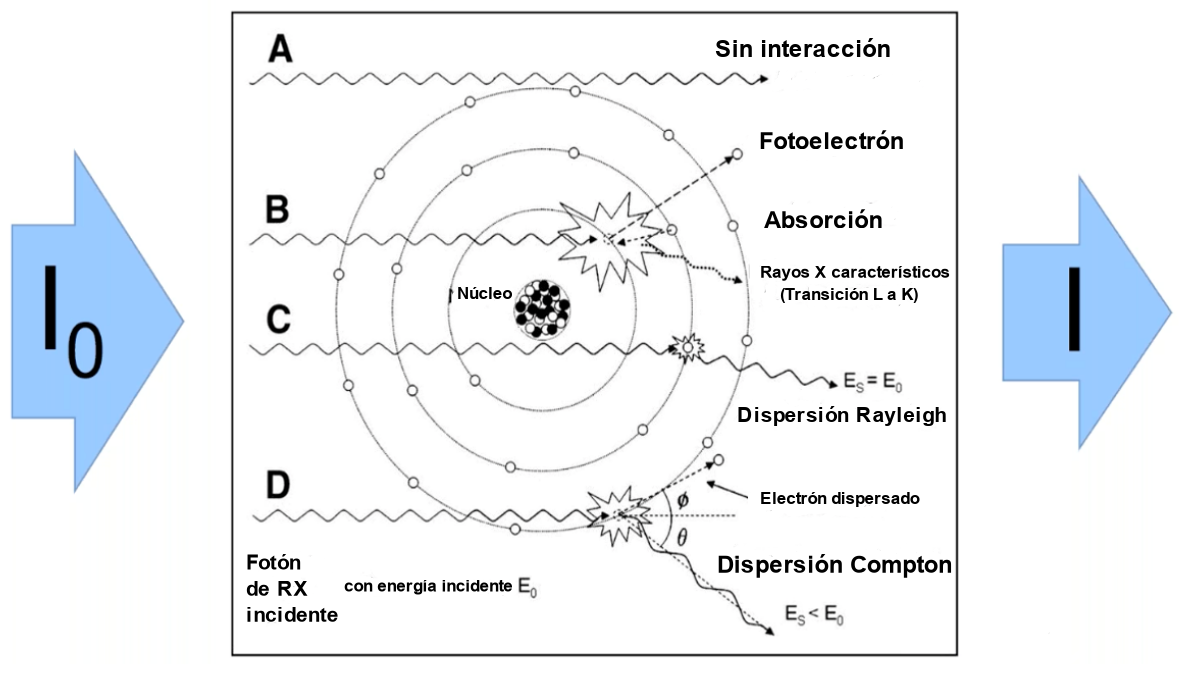
\includegraphics[width=0.6\textwidth]{images/interacciones.png}
    \caption{Posibles interacciones de fotones de rayos X (energías entre 0.1 y 200 keV), ya
    sea con electrones externos, internos o con núcleos.}
    \label{fig:interacciones}
\end{figure}

Si el blanco atenuador está compuesto por $N$ elementos en concentraciones másicas
dadas por $C_i = m_i/\sum_{i=1}^{N}m_i$ (con $m_i$ la masa del elemento $i$),
se puede considerar que el espesor $\Delta x$ está compuesto por distintas capas
de espesores $\Delta x_i$, correspondientes a cada elemento, para obtener un $\mu$
total de la forma

\begin{equation}
    \mu = \rho \sum_{i=1}^{N} \frac{\mu_i}{\rho_i} C_i
    \label{eq:mu_total}
\end{equation}

Por otro lado, la ecuación \ref{eq:atenuacion} es válida solo para un haz monocromático,
es decir, con una única energía $E$ en todos sus fotones. Sin embargo, en la mayoría
de los casos (sobre todo en la adquisición de radiografías), se suele trabajar con un
haz policromático con una distribución de energía $I_0(E)$ incidente. De esta forma, cada
fotón se atenuará con una proporción distinta, en función de $\mu(E)$, obteniéndose
que la intensidad resultante del haz tras atravesar un espesor $t$ es

\begin{equation}
    I = \int I_0(E) e^{-\mu(E,Z)t} dE
    \label{eq:policrom}
\end{equation} \cite{Als-Nielsen2011}

En general, se observa experimentalmente que $\mu(E,Z)$ disminuye cuando la energía
$E$ del haz aumenta (siendo
$Z$ los elementos que componen la muestra). Es decir, mientras más energía tengan los fotones, menor es
la probabilidad de que ocurra alguna interacción con la materia que atraviesan,
como se observa en la figura \ref{fig:coef_abs_agua}, para el agua.

\begin{figure}[htpb]
    \centering
    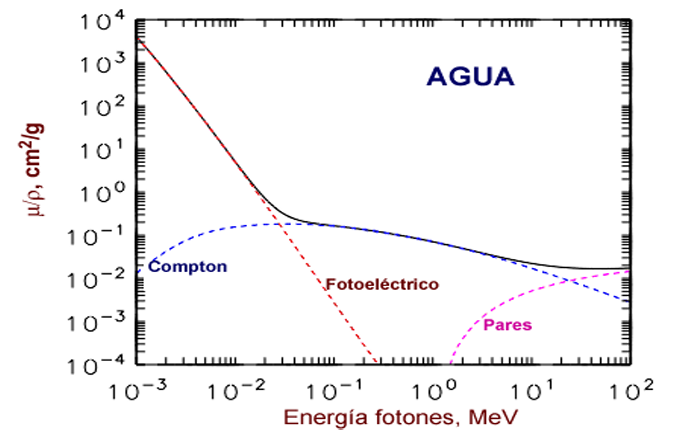
\includegraphics[width=0.5\textwidth]{images/coef_abs_agua.png}
    \caption{Coeficiente de atenuación másico $\mu / \rho$ del agua, en función
    de la energía $E$ del haz incidente.}
    \label{fig:coef_abs_agua}
\end{figure}

\subsection{Imágenes Radiográficas}

El proceso de obtención de una radiografía consta de 3 partes: la producción del haz de
rayos X, la interacción con la muestra y la adquisición en sí de la imagen a través
de un detector. La producción del haz se realiza con una fuente de rayos X, un
dispositivo que contiene un ánodo y un cátodo inmersos en un vacío dentro de un tubo (fig. \ref{fig:fuente}.a). El cátodo tiene
en su extremo un filamento que emite electrones al calentarse por una corriente.
Dichos electrones son acelerados mediante un voltaje (del orden de kV) hacia el ánodo,
cuyo extremo suele ser de tungsteno o molibdeno. Al impactar los electrones contra este blanco,
se emiten rayos X característicos (propios del material del ánodo) y radiación de
frenado, que salen del tubo como un haz cónico al pasar por una ventana de
berilio (material que absorbe muy poco los rayos X). Debido a las interacciones
que participan en el proceso, el haz resultante es policromático, con una distribución
de energía continua y con los picos característicos correspondientes (ver figura
\ref{fig:fuente}.b). Cambiando
el voltaje, se puede modificar la energía media del haz, y controlando la corriente
aplicada se puede aumentar o disminuir la cantidad de fotones generados (es decir,
la intensidad).

\begin{figure}[htpb]
    \centering
    \begin{subfigure}{0.3\textwidth}
        \centering
        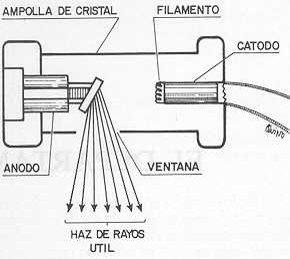
\includegraphics[width=\textwidth]{images/fuente_a.jpg}
        \caption{}
    \end{subfigure}
    \hspace{10mm}
    \begin{subfigure}{0.5\textwidth}
        \centering
        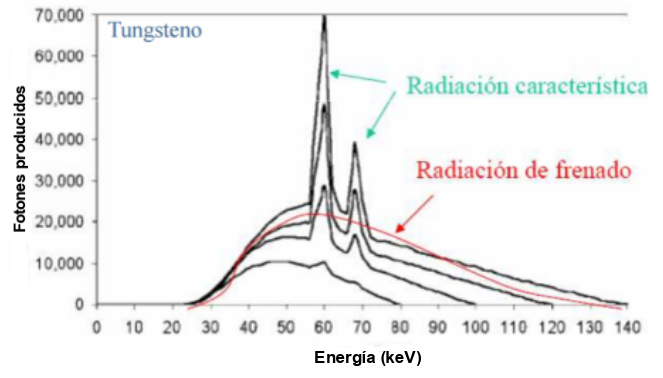
\includegraphics[width=\textwidth]{images/espectro_teorico.png}
        \caption{}
    \end{subfigure}
    \caption{Esquemas de producción de rayos X. (a) Se calienta el filamento a través
        de una corriente, emitiendo electrones que son acelerados hacia el ánodo a partir
        de una diferencia de potencial. Al impactar contra este, se generan rayos X por
        radiación de frenado y emisión de fotones característicos (b).}
    \label{fig:fuente}
\end{figure}

El haz obtenido sale de la fuente y atraviesa la muestra, ocurriendo en su interior
todas las interacciones mencionadas en la sección anterior (fig. \ref{fig:interacciones}). Así se va atenuando
hasta salir del objeto y alcanzar el detector digital. Este último registra la
cantidad de fotones que traspasaron la muestra sin interactuar a través de una
grilla cuadriculada de foto-diodos individuales (el tipo de detector de
pantalla plana más común) o una capa de un fotoconductor. Cada celda del detector produce una
señal eléctrica proporcional a la cantidad de fotones que reciben en un determinado
tiempo. Esto es interpretado digitalmente como pixeles con distintas tonalidades de gris. \cite{Stock2019}

En la figura \ref{fig:radiografia_mod} se puede observar con mayor detalle el proceso con
un esquema simplificado.
Un haz policromático de intensidad $I_0(E)$ interactúa con un volumen de espesor
$t$, en la posición $(x,y)$, con un coeficiente de atenuación $\mu(x,y;E,Z)$. Tras atenuarse, el haz que llega al
pixel $(x,y)$ del detector tiene una intensidad $I(x,y)$ dada por la ecuación $\ref{eq:policrom}$.
\medskip
\medskip

\begin{figure}[htpb]
    \centering
    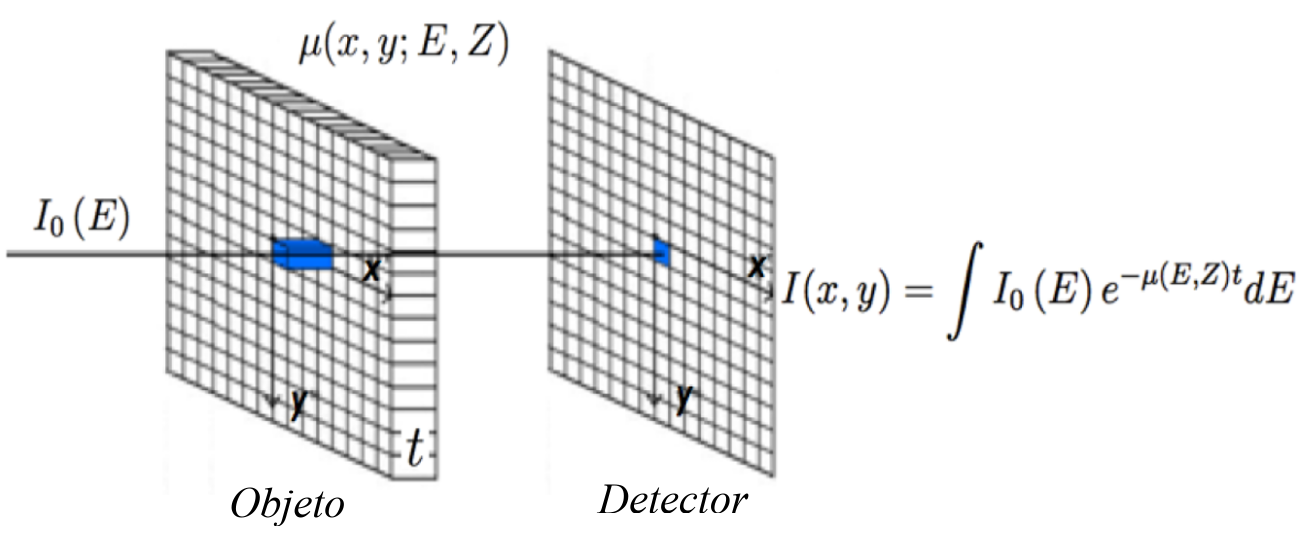
\includegraphics[width=0.6\textwidth]{images/radiografia_mod.png}
    \caption{Esquema simplificado del proceso de adquisición de una radiografía. Un haz de rayos X con intensidad $I_0(E)$
    atraviesa un volumen de espesor $t$ y coeficiente de absorción $\mu(x,y;E,Z)$. Tras interactuar
    con la materia, se atenúa y llega al pixel $(x,y)$ del detector con una intensidad $I(x,y)$.}
    \label{fig:radiografia_mod}
\end{figure}

Como puede observarse en la figura \ref{fig:radiografia_mod}, cada pixel de la imagen
obtenida, se asocia a un volumen (voxel) de la muestra, de las mismas dimensiones
en la sección transversal y de espesor $t$. Las diferencias de intensidad detectada,
o el ``contraste'' que se observa en la imagen, es el resultado de las variaciones
del coeficiente de atenuación en la muestra y/o las variaciones de espesor. Por lo
tanto, se define el \textit{contraste} en la imagen como la cantidad $\mu(E,Z)\cdot t$.
De esta forma, se puede obtener información de la estructura interna de una muestra
de composición variada y con distintos espesores, por ejemplo la mano de la figura
\ref{fig:radiografia_mano}, que contiene tejido duro, (hueso), y tejido blando
(músculo, piel, etc.). Sin embargo, la información que se puede extraer de una
radiografía es limitada por esta razón: sin un conocimiento previo de la muestra,
es imposible determinar solo el espesor $t$ o solo el coeficiente $\mu(E,Z)$,
y dos pixeles podrían tener la misma tonalidad de gris (contraste), y tener valores de
$t$ y $\mu$ completamente distintos. Así, se puede definir una radiografía como
una \textit{proyección de $\mu$ en la dirección del haz} sobre el plano del detector.

\begin{figure}[htpb]
    \centering
    \begin{subfigure}{0.24\textwidth}
        \centering
        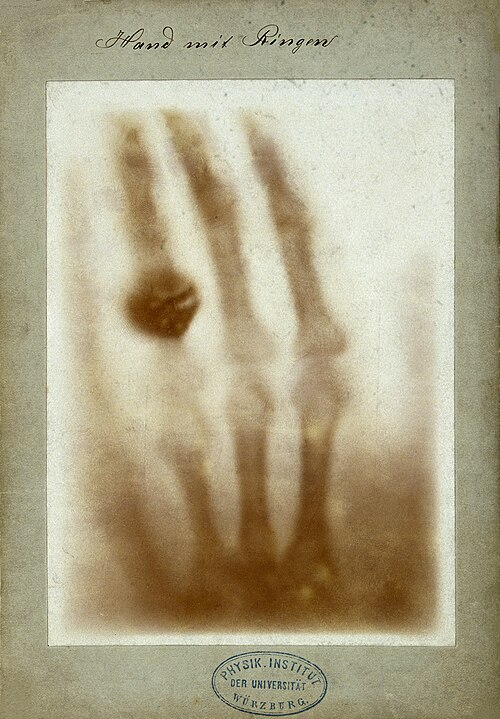
\includegraphics[width=\textwidth]{images/first_radiog.jpg}
    \end{subfigure}
    \hspace{10mm}
    %\hfill
    \begin{subfigure}{0.31\textwidth}
        \centering
        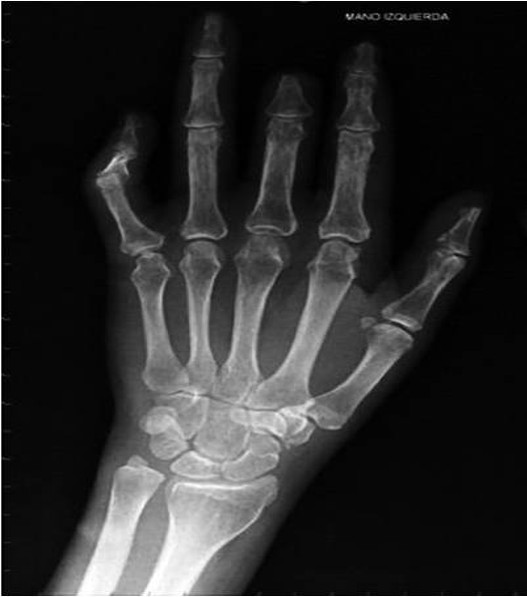
\includegraphics[width=\textwidth]{images/radiografia_mano.jpg}
    \end{subfigure}
    \caption{Primera radiografía de la historia, obtenida por W.C. Röntgen en 1895, de
    la mano de su esposa (izq.). Radiografía moderna de una mano humana (der.).}
    \label{fig:radiografia_mano}
\end{figure}

\subsection{Imágenes tomográficas}

Una tomografía es un \textit{mapa tridimensional del coeficiente de absorción $\mu$
de la muestra}, por lo que está exenta de las limitaciones propias de las
radiografías. Sin embargo, su adquisición requiere la obtención de múltiples
imágenes radiográficas de la muestra, llamadas proyecciones, en distintas direcciones
(realizando un barrido angular de $180^{\circ}$ o 360$^{\circ}$, con una distancia angular
constante entre cada imagen). Luego, la reconstrucción tomográfica se realiza por
cortes o \textit{slices} en el plano perpendicular al eje de rotación (eje $z$ de
la muestra), tal que para cada altura $z$ se toma la información de todas las proyecciones
y se procesan para obtener una imagen del coeficiente $\mu(x,y)$.

Por último, se agrupan todas las \textit{slices} reconstruidas y se ``apilan'' para formar
un mapa tridimensional del coeficiente de absorción $\mu(x,y,z)$, representado por
un valor numérico (un tono de gris) correspondiente al voxel $(x:x+\Delta x, y:
y+\Delta y, z:z+\Delta z)$, y que puede visualizarse como un modelo 3D mediante
algún software especializado.

La reconstrucción tomográfica es posible a partir de los teoremas y la transformada
de Radon, introducidas en 1917 por el matemático J. Radon. Se define la transformada
bidimensional de Radon de la función $f(x,y)$ como

\begin{equation}
    p(\xi, \gamma) = R_2 \{f(x,y)\} = \int f(\xi,\eta)d\eta
    \label{eq:transformada_radon}
\end{equation}

\noindent donde para cada ángulo $\gamma$ se definen los ejes perpendiculares $\xi$ y $\eta$,
y para cada coordenada $\xi$ se realiza la integral de línea en la dirección
de $\eta$, como se muestra en la figura \ref{fig:transf_radon}. Por otro lado,
el teorema de Radon afirma que \textit{su transformada es invertible.} Es decir
se puede reconstruir la función $f(x,y)$ a partir de su transformada. \cite{Als-Nielsen2011}

\begin{figure}[htpb]
    \centering
    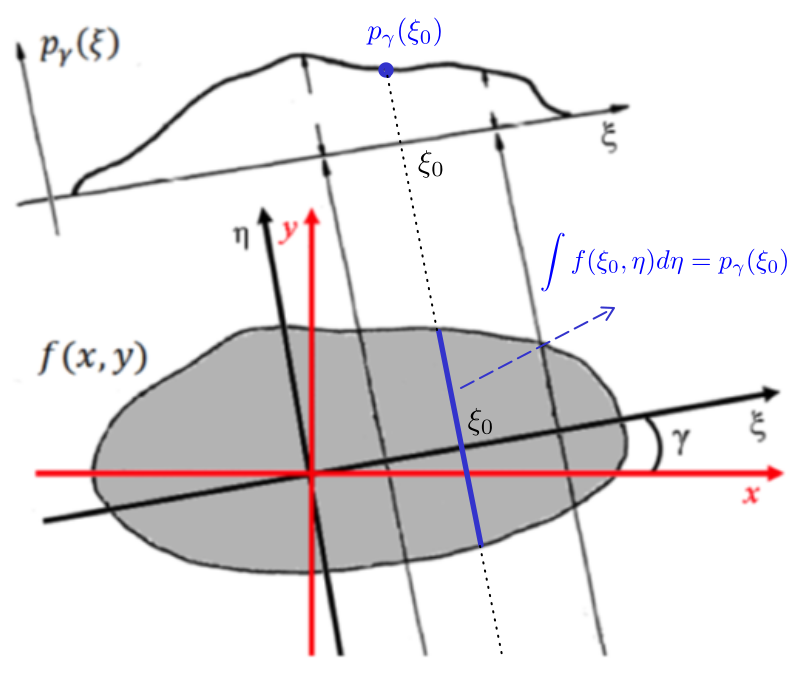
\includegraphics[width=0.5\textwidth]{images/transf_radon.png}
    \caption{Esquema de la transformada de Radon. Para cada ángulo $\gamma$ entre 
    el eje $x$ y un eje $\xi$, se obtiene una proyección $p_\gamma(\xi)$, que 
    es la integral de línea de $f(x,y)$ en la dirección $\eta$ (perpendicular a $\xi$).
    En el caso de una tomografía, la dirección $\eta$ es la dirección del haz de rayos X
    paralelos que atraviesan la muestra para una proyección específica.}
    \label{fig:transf_radon}
\end{figure}

Si se considera un haz monocromático que atraviesa una muestra (con $\mu(x,y)$
variable en el espesor), en una dirección perpendicular al eje $\xi$ (coplanar
con $x$ e $y$), entonces la proyección radiográfica de un solo corte transversal
es una línea de pixeles \{px$_1$, px$_2$, ..., px$_{\xi}$\} con intensidades $I(\xi)$ dadas por la ecuación

\begin{equation}
    I(\xi) =  I_0(\xi)e^{-\int \mu(\xi,\eta)d\eta}
    \label{eq:proyeccion}
\end{equation}

\noindent donde la integral se realiza sobre el espesor atravesado en la dirección del haz.
De esta forma, podemos despejar y obtener la transformada de Radon de $\mu(x,y)$.

\begin{equation}
    -ln\left(\frac{I(\xi, \gamma)}{I_0}\right) = \int \mu(\xi,\eta)d\eta = R_2\{\mu(x,y)\}
    \label{eq:transf_mu}
\end{equation}

Así, se puede medir el parámetro $\ln(I(\xi, \gamma)/I_0)$ (para todos los ángulos $\gamma$) y anti-transformarlo para
obtener el mapa bidimensional de $\mu(x,y)$ para ese plano. Repitiendo el proceso
para todos los planos en $z$, se obtiene una reconstrucción tomográfica completa.
La necesidad de múltiples proyecciones, en distintos ángulos, radica en que la
transformada de Radon de $\mu(x,y)$ es una función $p(\xi,\gamma)$, con $\gamma$
el ángulo de la proyección (fig. \ref{fig:transf_radon}). \cite{Als-Nielsen2011}

% Para la representación de los resultados es común utilizar las unidades de Hounsfield
% ($HU$), donde se relaciona el coeficiente de absorción $\mu$ del material con el
% del agua ($\mu_{agua}$).

% \begin{equation}
%     HU = \dfrac{\mu - \mu_{agua}}{\mu_{agua}}
%     \label{eq:HU}
% \end{equation}

El teorema de Radon es la demostración matemática y el fundamento detrás de la reconstrucción
tomográfica a partir de proyecciones, sin embargo, calcular la anti-trans\-for\-ma\-da
del logaritmo explicítamente no es algo trivial, y generalmente implica un alto
costo computacional. Para ello, se han implementado distintos métodos y aproximaciones
que facilitan la tarea. Entre ellos, el más usado y extendido, por ser rápido,
sencillo y eficiente, es el algoritmo de \textit{Retro-proyección filtrada}. Este
funciona siempre y cuando la intensidad transmitida (el número de cuentas) sea 
alta, algo usual en la mayoría de tomografías de rayos X. \cite{Stock2019}\cite{Als-Nielsen2011}

Por otro lado, la transformada de Radon es una función $p(\xi,\gamma)$ que depende del ángulo
$\gamma$ de la proyección, como se mencionó antes, y esto implica la necesidad de múltiples
proyecciones. Lo mismo sucede para cualquier algoritmo de reconstrucción.
El mínimo número de proyecciones (MNP), está dado por el \textit{Teorema de muestreo
de Nyquist-Shanon} \cite{Nyquist}, el cual dice que para mantener la resolución del detector, haciendo
un barrido de 180$^{\circ}$, el MNP debe ser igual al número de pixeles que ocupa el ancho
(perpendicular al eje de rotación) de la región de interés en la imagen.

\subsection{Micro-radiografía y micro-tomografía}

Las figuras \ref{fig:radiografia_mod} y \ref{fig:transf_radon} son válidas cuando
los rayos X incidentes son paralelos entre sí. Sin embargo, debido al diseño de
las fuentes más comúnmente usadas, esto no suele ser la norma en los tomógrafos, sino que se suele trabajar
con haces cónicos o haces de tipo abanico (similar al cónico, pero los rayos solo
se propagan en un mismo plano) cuyo foco es la sección del ánodo, de la que se emiten los fotones.
Si la región de interés es muy pequeña y se encuentra
en el área central del cono/abanico, entonces los rayos pueden aproximarse como
paralelos, pero incluso si este no es el caso, los métodos de la anti-transformada
de Radon y la retro-proyección filtrada pueden adaptarse sin mucha dificultad a
la geometría. Pero la utilidad de un haz cónico va más allá del diseño de la fuente,
y es la posibilidad de realizar una magnificación de la imagen, permitiendo explorar
detalles muy pequeños de la muestra, con alta resolución espacial. Los avances
tecnológicos han permitido diseñar microtomógrafos capaces de detectar detalles
del orden 1 $\mu$m, e incluso, centenas de nm (llamados ``nanotomógrafos'' \cite{Claro2023}).

El fundamento detrás de esto está en el tratamiento de los rayos X emitidos, bajo la
óptica geométrica, teniendo en cuenta que, a diferencia de la luz visible, los rayos X no proyectan sombras opacas debido a
su capacidad de atravesar la materia. Así, se define la magnificación $M$ de un sistema
de micro-tomografía como

\begin{equation}
    M = \frac{\Delta x_{proy}}{\Delta x_{real}} = \frac{D}{F}
    \label{eq:magnificacion}
\end{equation}

\noindent donde $\Delta x_{real}$ es una distancia en alguna dirección (arbitraria, pero en un
plano paralelo al detector) de la muestra, y $\Delta x_{proy}$ es la distancia correspondiente
a $\Delta x_{real}$ que se proyecta directamente sobre el detector para obtener
una imagen radiográfica. Por otro lado, $D$ y $F$ son las distancias fuente-detector
y fuente-objeto respectivamente, de acuerdo con las consideraciones de la óptica geométrica.

Se entiende por \textit{resolución espacial} ($RE$) a la distancia mínima entre dos elementos de la muestra
que al proyectarse sobre el detector (o al reconstruirse, si hablamos de tomografía),
pueden distinguirse como elementos distintos. También suele medirse desde el dominio de
las frecuencias espaciales, como lp/mm (``pares de línea por milímetro'') o ciclos/mm,
es decir, la cantidad de ciclos de una frecuencia espacial (por ejemplo, líneas blancas
y negras) que pueden distinguirse en una distancia determinada. En general, la resolución espacial de un microtomógrafo
está determinada por todos los procesos de ``transferencia'' de señal que ocurren en una
adquisición: desde la producción y colimación inicial de los rayos X, sus interacciones
con la muestra, su interacción con el centellador (si el detector tiene) e interacción con los foto-diodos, el proceso de transformación
a una señal eléctrica, la digitalización de esta misma, y el algoritmo de reconstrucción.

Cada uno de estos procesos altera la señal original y funciona como un ``filtro'' que
difumina los detalles de la muestra \cite{Buzug2008}. Sin embargo no todos tienen el mismo peso, y en
los microtomógrafos actuales, los factores más influyentes son la magnificación $M$ del
sistema, el tamaño del pixel $\Delta p$ del detector y el tamaño focal $S$ (diámetro del foco,
el área desde donde se emiten los rayos X).
Los primeros dos pueden entenderse a partir de la ecuación \ref{eq:magnificacion}, siendo
$\Delta p = M \Delta x_{min}$ la magnificación de la distancia mínima distinguible cuando
la fuente es puntual. Pero en realidad las fuentes no son puntuales, lo que implica también un
área de ``penumbra'' en los bordes. Luego, se utiliza la siguiente expresión como aproximación
de la resolución espacial de un microtomógrafo. \cite{JunYan2010}

\begin{equation}
    RE = \sqrt{\left(S\dfrac{M-1}{M}\right)^2 + \left(\frac{\Delta p}{M}\right)^2} 
    \hspace{10mm} [\text{lp/mm}] = \frac{1}{2\cdot RE[\text{mm}]} 
    \label{eq:res_espacial}
\end{equation}

\noindent donde el factor $1/2$ en la conversión a lp/mm está relacionado a la frecuencia de corte
o frecuencia de Nyquist, que es la frecuencia máxima que puede ser detectada por un 
sistema de muestreo \cite{Nyquist} \cite{Buzug2008}.

\subsection{Artefactos}

Se define como artefacto de una radiografía/tomografía con toda distorsión de la imagen
que dificulte la visualización de las estructuras propias del objeto. Suelen
presentarse como rayas, ruido, alteraciones de la arquitectura, anillos, bandas
blancas y negras superpuestas, entre otros (ver figura \ref{fig:artefactos}); y 
tienen tres orígenes posibles: físico, cinético y técnico. A continuación se 
mencionarán algunos de los más pertinentes para este trabajo:

\begin{itemize}
    \item Volumen parcial (físico): si la muestra tiene un cambio de contraste brusco, un
    borde ``filoso'', este se digitalizará como un cambio lineal de intensidad en varios
    pixeles, efectivamente mostrando un borde borroso. Esto se debe a que las
    intensidades calculadas para cada pixel tienen cierta dependencia de los valores de
    sus vecinos, y también a los procesos de reconstrucción empleados. Además, otro factor
    en juego es el tamaño de foco de la fuente (que no es puntual), que genera un efecto
    de ``penumbra'' \cite{Buzug2008}.
    \item Endurecimiento del haz (físico): a menor energía, más probable es la
    interacción de un fotón con la materia, por lo tanto, cuando un haz policromático
    atraviesa un material, serán estos fotones los que sean absorbidos con más frecuencia.
    Así, la distribución de energía del haz incidente cambia capa a capa, y como $\mu(E)$
    depende de la energía, se medirá un $\mu$ menor al real, mientras mayor sea el
    espesor (incluso si el material es homogéneo y uniforme en toda la muestra) \cite{Buzug2008}.
    \item Baja tasa de conteo (físico): si la muestra es de gran espesor, o atenúa mucho,
    los fotones que llegan al detector son muy pocos como para apreciar el contraste \cite{Buzug2008}. 
    \item Movimientos del objeto (cinético): el proceso de reconstrucción tomográfica asume
    que la muestra no se traslada en el espacio, solo rota sobre su eje \cite{Buzug2008}. 
    \item Movimientos del sistema (cinético): también se asume que los elementos del sistema
    están fijos en el espacio, en relación a la muestra \cite{Buzug2008}. 
    \item Desalineaciones del sistema (técnico): todo algoritmo de reconstrucción asume ciertas
    características de la geometría del sistema, como la posición relativa entre los componentes,
    posibles inclinaciones, etc. Si estas no se cumplen, se producen distorsiones en la imagen
    reconstruida. Las posibles desalineaciones serán abordadas con mayor detalle en el capítulo
    \ref{cap:cal_espacial} \cite{Buzug2008} \cite{Sun2006}.
\end{itemize}

El objetivo principal de este trabajo es reducir este último tipo de artefactos, que son
altamente influyentes en las reconstrucciones tomográficas, por medio de métodos que se
detallan en el capítulo \ref{cap:cal_espacial}.

% \begin{figure}[h]
%     \centering
%     \begin{subfigure}[b]{0.36\textwidth}
%         \centering
%         
\includegraphics[width=\linewidth,keepaspectratio]{images/artefacto1.png}
%         \caption{Imagen 1}
%     \end{subfigure}
%     \hfill
%     \begin{subfigure}[b]{0.62\textwidth}
%         \centering
%         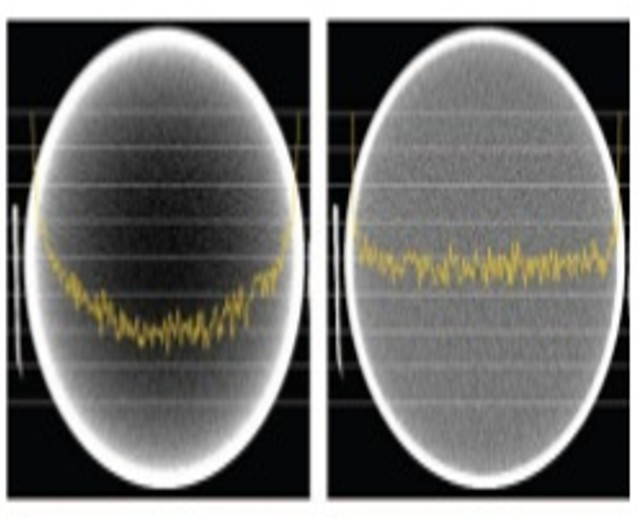
\includegraphics[width=\linewidth,keepaspectratio]{images/artefacto2.jpg}
%         \caption{Imagen 2}
%     \end{subfigure}

%     \vspace{3mm}

%     \begin{subfigure}[b]{0.38\textwidth}
%         \centering
%         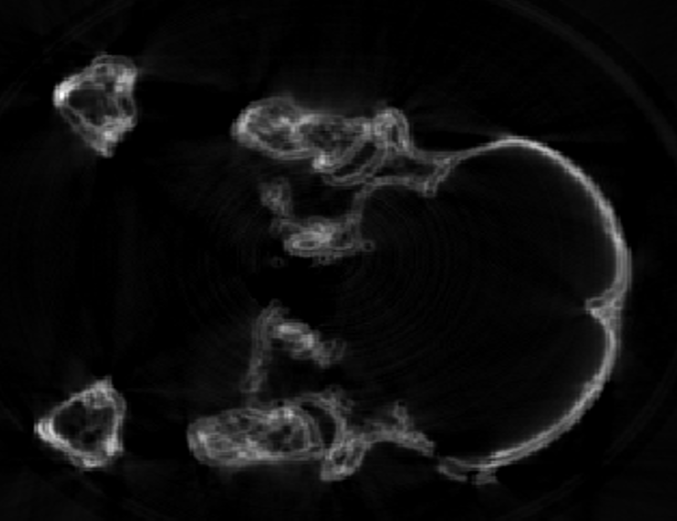
\includegraphics[width=\linewidth,keepaspectratio]{images/artefacto3.png}
%         \caption{Imagen 3}
%     \end{subfigure}
%     \hfill
%     \begin{subfigure}[b]{0.60\textwidth}
%         \centering
%         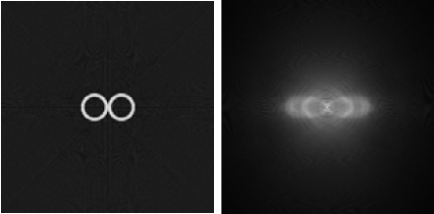
\includegraphics[width=\linewidth,keepaspectratio]{images/artefacto4.png}
%         \caption{Imagen 4}
%     \end{subfigure}
%     \caption{Algunos artefactos comunes en radiografías y tomografías. (a) Volumen parcial;
%     (b) y (c) endurecimiento del haz; (d) Movimientos del sistema/objeto; y (e) artefacto por
%     desalineación del sistema, en concreto, por una inclinación del detector.}
%     \label{fig:artefactos}
% \end{figure}

\begin{figure}[htpb]
    \centering
    \begin{subfigure}[b]{0.3\textwidth}
        \centering
        \begin{overpic}[width=\linewidth]{images/artefacto1.png}
            \put(3,70){\colorbox{black!60}{\color{white}\bfseries\large (a)}}
        \end{overpic}
    \end{subfigure}
    \hspace{2mm}
    \begin{subfigure}[b]{0.5\textwidth}
        \centering
        \begin{overpic}[width=\linewidth]{images/artefacto2.png}
            \put(3,40){\colorbox{black!60}{\color{white}\bfseries\large (b)}}
            \put(53,40){\colorbox{black!60}{\color{white}\bfseries\large (c)}}
        \end{overpic}
    \end{subfigure}

    \vspace{2mm}

    \begin{subfigure}[b]{0.3\textwidth}
        \centering
        \begin{overpic}[width=\linewidth]{images/artefacto3.png}
            \put(3,65){\colorbox{black!60}{\color{white}\bfseries\large (d)}}
        \end{overpic}
    \end{subfigure}
    \hspace{2mm}
    \begin{subfigure}[b]{0.50\textwidth}
        \centering
        \begin{overpic}[width=\linewidth]{images/artefacto4.png}
            \put(3,40){\colorbox{black!60}{\color{white}\bfseries\large (e)}}
            \put(53,40){\colorbox{black!60}{\color{white}\bfseries\large (f)}}
        \end{overpic}
    \end{subfigure}
    \caption{Algunos artefactos comunes en radiografías y tomografías. (a) Borde difuso por
    volumen parcial; (b) endurecimiento del haz en un cilindro homegéneo (c); (d) distorsiones
    en la imagen por movimientos del sistema/objeto;(e) es una imagen correspondiente a un
    sistema bien alineado, y (f) la misma imagen pero con un artefacto por
    desalineación del sistema, en concreto, por una inclinación del detector.}
    \label{fig:artefactos}
\end{figure}


\subsection{Una figura recurrente: la elipse}

Debido a la forma cónica del haz, y a las trayectorias circulares que realizan elementos
de la muestra durante la rotación, es común que las proyecciones radiográficas contengan
formas elípticas, por lo que es necesario tener en cuenta algunos conceptos útiles, tanto
para la alineación del sistema, como para el procesamiento digital.

Una elipse es una curva plana, simple y cerrada, que contiene puntos focales tales que,
para todos los puntos de la curva, la suma de las distancias a ambos focos es constante.
Es la generalización de la circunferencia, que es un tipo especial de elipse cuyos focos
coinciden en un mismo punto. Los diámetros más largo y más corto se denominan respectivamente,
el eje mayor (o \textit{ancho}) y el eje menor (o \textit{altura}), y se denotan por $2a$ y $2b$
(ver figura \ref{fig:elipse}.a). Los cuatro puntos de la curva que se ubican sobre estos ejes principales se conocen como 
\textit{vértices}. Una elipse cuyos ejes principales están alineados con los ejes $x$ e $y$,
centrada en el origen, puede describirse mediante la siguiente ecuación:

\begin{equation}
    \frac{x^2}{a^2} + \frac{y^2}{b^2} = 1
    \label{eq:elipse_simple}
\end{equation}

La elipse puede definirse también como una de las curvas cerradas (la otra es el
círculo) que se pueden formar en la intersección de un plano y la superficie de un cono
circular (ver \ref{fig:elipse}.b). Esta definición es particularmente útil para
microtomógrafos de haz cónico, en los que la pantalla del detector es el plano que interseca con
el cono. La ecuación que describe este tipo de curvas es $\hat{A}x^2 + \hat{B}xy +
\hat{C}y^2 + \hat{D}x + \hat{E}y + \hat{F} = 0$, con $\hat{B}^2 - 4\hat{A}\hat{C} < 0$, y puede ser reescrita
como

\begin{equation}
    A(x-x_0)^2 + B(y-y_0)^2 + 2C(x-x_0)(y-y_0) = 1
    \label{eq:elipse}
\end{equation}

\noindent donde $x_0$ e $y_0$ son las coordenadas del centro de la elipse, y $A$, $B$ y $C$ son
parámetros relacionados con el ancho, la altura y la orientación. En concreto, la misma ecuación
puede ser entendida como un producto matricial, entre $\mathbf{x}=(x-x_0, y-y_0)$ y una
matriz $\mathbb{A}$ que contiene toda la información de la elipse \cite{Strang2016}.

\begin{equation}
    \mathbf{x}^T \mathbb{A} \mathbf{x} = 1, \hspace{5mm} \mathbb{A} = \begin{bmatrix}
        A & C \\
        C & B
    \end{bmatrix}
    \label{eq:elipse_matriz}
\end{equation}

Al ser $\mathbb{A}$ una matriz real y simétrica, puede ser diagonalizada mediante una rotación.
Específicamente, si se rota el sistema de coordenadas hasta coincidir los ejes principales
de la elipse con los ejes cartesianos, entonces

\begin{equation}
    \mathbf{x'}^T 
    \begin{bmatrix}
        \lambda_1 & 0 \\
        0 & \lambda_2
    \end{bmatrix}
    \mathbf{x'} = 1 \hspace{5mm }\Longrightarrow \hspace{5mm} \lambda_1 x'^2 +  \lambda_2 y'^2 = 1
     \label{eq:elipse_diagonal}
\end{equation}

\noindent donde $\lambda_1$ y $\lambda_2$ son los autovalores de $\mathbb{A}$ y, a partir de la ecuación
\ref{eq:elipse_simple}, se puede deducir que $a = 1/\sqrt{\lambda_1}$ y $b = 1/\sqrt{\lambda_2}$.
Por otro lado, los autovectores de dicha matriz definen las direcciones de los ejes principales.
En concreto, si se toman las coordenadas del vector correspondiente al eje mayor, $\mathbf{v}_a=(v_{a,x},v_{a,y})$,
se puede obtener el ángulo de dicho eje con respecto a $x$, a través de la siguiente expresión \cite{Strang2016}.

\begin{equation}
    \theta = \arctan\left(\frac{v_{a,y}}{v_{a,x}}\right) = \frac{1}{2} \arctan\left(\frac{2C}{A-B}\right)
    \label{eq:angulo_elipse}
\end{equation}


\begin{figure}[htpb]
    \centering
    \begin{subfigure}{0.35\textwidth}
        \begin{overpic}
            [width=\textwidth]{images/general_ellipse.png}
            \put(3,95){\colorbox{black!60}{\color{white}\bfseries\large (a)}}
        \end{overpic}
        
    \end{subfigure}
    \hspace{10mm}
    \begin{subfigure}{0.35\textwidth}
        \begin{overpic}
            [width=\textwidth]{images/ellipse_conic.png}
            \put(3,95){\colorbox{black!60}{\color{white}\bfseries\large (b)}}
        \end{overpic}

    \end{subfigure}
    \caption{(a) Forma general de una elipse en el plano, definida por sus semi-ejes $a$ y $b$,
    su centro $(x_0,y_0)$ y su ángulo de inclinación $\theta$. (b) La elipse como producto de la intersección
    entre un plano y la superficie de un cono circular.}
    \label{fig:elipse}
\end{figure}

La ``elongación'' de una elipse se mide a través de la \textit{excentricidad}, que se calcula como

\begin{equation}
    e = \frac{c}{a} = \sqrt{1 - \frac{b^2}{a^2}}
    \label{eq:excentricidad}
\end{equation}

\noindent donde $c$ es la distancia entre el centro y uno de los focos. Para una circunferencia, $e=0$
y para una elipse $0<e<1$. Es de interés para este trabajo definir los siguientes criterios de evaluación de
``similitud'' entre una elipse y una circunferencia: la \textit{circularidad de Wadell} $C_W$ y
la \textit{relación de aspecto} $R$ (ambos menores a 1, e iguales solo en el caso de una
circunferencia), y el ángulo $\alpha$ entre los respectivas secciones cónicas.

\begin{equation}
    C_W = \frac{4\pi \cdot Area}{Perim^2} \hspace{10mm} R = \frac{b}{a}
    \label{eq:circ_R}
\end{equation}


Volviendo a la definición de la elipse como una sección cónica, se puede determinar el ángulo
de inclinación $\alpha'$ del plano de la elipse, con respecto al eje principal del cono, a partir
de los semi-ejes $a$ y $b$. La excentricidad de una sección cónica, producida por la
intersección de dicho plano, viene dada por $e=\cos\alpha'/\cos\beta$, donde $\beta$ el
semi-ángulo de apertura del cono. Luego, igualando con la ecuación \ref{eq:excentricidad}, 
y cambiando de variable a $\alpha = \pi/2 - \alpha'$, se obtiene la siguiente expresión:

\begin{equation}
    \alpha = \arcsin\left(\cos\beta \cdot \sqrt{1 - R^2}\right)
    \label{eq:alfa_proyeccion}
\end{equation}

\noindent donde el ángulo $\alpha$ es la inclinación del plano de la elipse con respecto a un plano
perpendicular al eje del cono (cuya sección cónica es una circunferencia), con el eje menor
como su eje de rotación \cite{Meserve1983} \cite{Larson2006}. Este último parámetro sirve también
para caracterizar la similitud de una elipse con un círculo (mientras más cercano a cero, más similar),
y será utilizado en el proceso de alineación.

\section{Procesamiento digital de imágenes}

En términos matemáticos, una imagen puede ser representada por medio de una función
bidimensional $f(x,y)$ donde las coordenadas $(x,y)$ (pixeles) se corresponden
con la posición en el plano, y el valor funcional indica la intensidad $I(x,y)$
en ese punto (ver figura \ref{fig:img_digital}). Existen dos tipos de imágenes comúnmente utilizadas: imágenes en
tonos de grises e imágenes a color, diferenciándose según cómo $f(x,y)$ representa
a la intensidad. En el primer caso, a cada pixel le corresponde un valor entero $g$
perteneciente a una escala entre 0 y $g_{max}=2^n -1$ ($2^n$ se corresponde con un formato
de ``n-bits'' para obtener dicha escala), tal que 0 representa al color negro y $2^n -1$ al blanco, y todo
tono de gris, un valor entre estos. En el segundo caso, la función $f(x,y)$ es un
vector de tres componentes (rojo, verde y azul), donde cada componente puede tomar
un valor entre 0 y $g_{max}$. Para una imagen radiográfica, la función $f(x,y)$ está
asociada directamente a la cantidad de fotones detectados en el foto-diodo $(x,y)$
del detector, una cantidad que es escalar para cada ``pixel'', por lo tanto, esta se
representa con tonos de grises. \cite{Martinsanz}\cite{Gonzalez}

\begin{figure}[htpb]
    \centering
    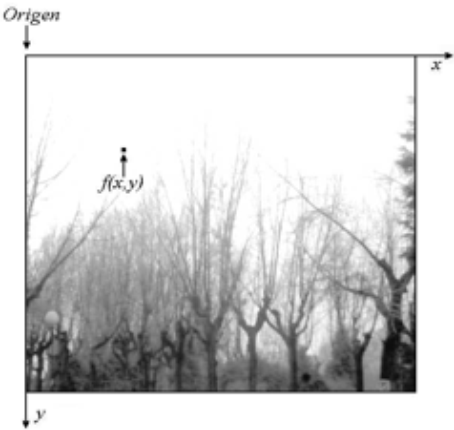
\includegraphics[width=0.45\textwidth]{images/img_digital.png}
    \caption{Representación matemática de una imagen digital. A cada pixel $(x,y)$ le
    corresponde un valor de intensidad dado por una función $f(x,y)$, escalar en el caso
    de tonos de gris, y vectorial en el caso de imágenes a color.}
    \label{fig:img_digital}
\end{figure}

\subsection{Conceptos estadísticos}

Una imagen típica puede contener millones de pixeles, sin embargo, sus valores de intensidad
no suelen ser totalmente aleatorios (para imágenes de objetos reales), por lo que es útil
analizarlos a partir de la estadística. A continuación, se definen algunos conceptos
estadísticos que se utilizaron en este trabajo.

\textit{Histograma} ($h(g)$):

El histograma de una imagen, o de una región de interés (ROI), es una función discreta que representa el número de
pixeles en la imagen en función de los niveles de grises $g$. $h(g)$ equivalente
a una distribución de probabilidad $P(g)$ de un determinado nivel de gris $g$.
Se define como

\begin{equation}
    h(g) = P(g) = n(g)/N 
    \label{eq:histograma}
\end{equation}

\noindent donde $n(g)$ es el número de pixeles con intensidad $g$, y $N$ es el número total
de pixeles en la imagen \cite{Martinsanz}. Al ser una distribución de probabilidad,
debe estar normalizada, es decir, $\sum_{g}h(g) = 1$. Esta función no brinda
información espacial, solo de la frecuencia de aparición de cada nivel de gris,
sin embargo, puede utilizarse para realizar segmentaciones. En la figura \ref{fig:histograma_ej}
puede encontrarse un ejemplo concreto.
\\

\begin{figure}[htpb]
    \centering
    \begin{subfigure}{0.35\textwidth}
        \begin{overpic}
            [width=\textwidth]{images/artefacto1.png}
            \put(2,74){\colorbox{black!60}{\color{white}\bfseries\large (a)}}
        \end{overpic}
        
    \end{subfigure}
    \hspace{10mm}
    \begin{subfigure}{0.40\textwidth}
        \begin{overpic}
            [width=\textwidth]{images/histograma_ej.png}
            \put(3,65){\colorbox{black!60}{\color{white}\bfseries\large (b)}}
        \end{overpic}

    \end{subfigure}
    \caption{Imagen de 632880 pixeles, en escala de grises 8-bit, con dos regiones bien marcadas
    (\textbf{a}) y su histograma (\textbf{b}).}
    \label{fig:histograma_ej}
\end{figure}

\textit{Valor Medio} ($VM$):

El valor medio de un ROI se define como el promedio de intensidades obtenidas,
y se calcula como

\begin{equation}
    VM = \langle I \rangle = \sum_{g=0}^{g_{max}}g\cdot h(g) = \sum_{x}\sum_{y}\frac{I(x,y)}{N}
    \label{eq:VM}
\end{equation}

\noindent donde $I(x,y)$ es la intensidad en el pixel $(x,y)$ \cite{Martinsanz}.
\\

\textit{Desviación Estándar (DS)}:

La $DS$ es una medida de dispersión de los valores de intensidad respecto al
valor medio, y se calcula mediante la siguiente expresión \cite{Martinsanz}

\begin{equation}
    DS^2 = \sum_{g=0}^{g_{max}}(g-VM)^2h(g) = \sum_{x}\sum_{y}\frac{(I(x,y)-VM)^2}{N}
    \label{eq:DS}
\end{equation}\\

\textit{Relación Señal Ruido (SNR)}:

Relación entre la señal (representada por $I$, el número de fotones detectados)
y el ruido estadístico asociado al proceso de adquisición $\sigma$
\cite{Martinsanz} \cite{Gonzalez}. Se considera como SNR de un ROI el valor medio
de los SNR de todos los pixeles del ROI.

\begin{equation}
    SNR = \left\langle \frac{I(x,y)}{\sigma} \right\rangle
    \label{eq:SNR}
\end{equation}

Cuando el $SNR$ toma valores pequeños, el ruido estadístico es comparable con la
intensidad detectada (ver figura \ref{fig:SNR}). El criterio de Rose afirma que para poder distinguir las
características de la imagen con 100$\%$ de certeza es necesario que el $SNR$
tome valores mayores a 5 \cite{Bushberg}.\\

\begin{figure}[htpb]
    \centering
    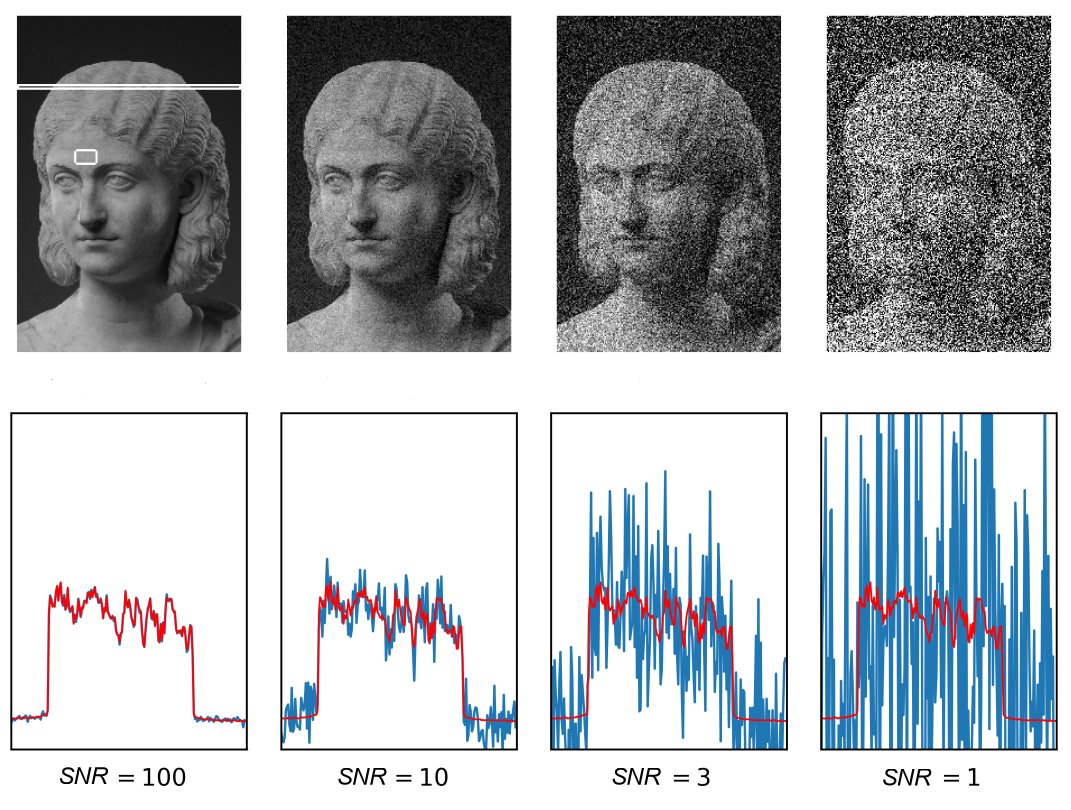
\includegraphics[width=0.70\textwidth]{images/SNR.png}
    \caption{Visualización de distintos niveles de $SNR$ para una misma imagen.}
    \label{fig:SNR}
\end{figure}

\textit{Relación Constraste Ruido (CNR):}

Se define el $CNR$ entre los puntos A y B de un ROI como el contraste de
intensidades entre dichos puntos $I_A - I_B$ sobre el ruido estadístico asociado
al proceso de adquisición $\sigma$ \cite{Bushberg}. Representa la
capacidad de distinguir la variación de intensidades entre las dos regiones de
la imagen.

\begin{equation}
    CNR = \frac{I_A - I_B}{\sigma}
    \label{eq:CNR}
\end{equation}

\subsection{Transformaciones Geométricas}

El análisis y la corrección de desalineaciones de un microtomógrafo requiere saber cómo se
puede transformar una imagen al considerarla como un elemento geométrico. Una 
transformación geométrica de una imagen es una operación que redefine la
disposición espacial de los datos sin alterar (idealmente) la naturaleza de la
información capturada. Estas transformaciones pueden describirse según qué propiedades del objeto original
preservan. Algunos ejemplos pertinentes para este trabajo son los siguientes (ver
figura \ref{fig:transformaciones}).

\begin{enumerate}[label=\alph*)]
    \item \textit{Isometrías}: Preservan distancias y ángulos (rotación y traslación).
    \item \textit{Similitudes}: Preservan la forma pero cambian el tamaño (escalado).
    \item \textit{Afines}: Preservan el paralelismo (shear).
    \item \textit{Proyectivas}: No preservan ángulos ni paralelismo; solo preservan la
    colinealidad (cambios de perspectiva).
\end{enumerate}

\begin{figure}[htpb]
    \centering
    \begin{subfigure}{0.25\textwidth}
        \begin{overpic}
            [width=\textwidth]{images/normal_im.png}
            \put(3,82){\colorbox{black!60}{\color{white}\bfseries\large (a)}}
        \end{overpic}
    \end{subfigure}
    \hspace{3mm}
    \begin{subfigure}{0.25\textwidth}
        \begin{overpic}
            [width=\textwidth]{images/rotation.png}
            \put(3,82){\colorbox{black!60}{\color{white}\bfseries\large (b)}}
        \end{overpic}
    \end{subfigure}
    \hspace{3mm}
    \begin{subfigure}{0.25\textwidth}
        \begin{overpic}
            [width=\textwidth]{images/translation.png}
            \put(3,82){\colorbox{black!60}{\color{white}\bfseries\large (c)}}
        \end{overpic}
    \end{subfigure}
    \vspace{2mm}
    \begin{subfigure}{0.25\textwidth}
        \begin{overpic}
            [width=\textwidth]{images/scale.png}
            \put(3,82){\colorbox{black!60}{\color{white}\bfseries\large (d)}}
        \end{overpic}
    \end{subfigure}
    \hspace{3mm}
    \begin{subfigure}{0.25\textwidth}
        \begin{overpic}
            [width=\textwidth]{images/shear.png}
            \put(3,82){\colorbox{black!60}{\color{white}\bfseries\large (e)}}
        \end{overpic}
    \end{subfigure}
    \hspace{3mm}
    \begin{subfigure}{0.25\textwidth}
        \begin{overpic}
            [width=\textwidth]{images/projective.png}
            \put(3,82){\colorbox{black!60}{\color{white}\bfseries\large (f)}}
        \end{overpic}
    \end{subfigure}
    \caption{Algunas de las principales transformaciones geométricas de una imagen.
    (a) Imagen original. (b) Rotación isométrica afín. (c) Traslación isométrica afín.
    (d) Escalado. (e) Shear. (f) Cambio de perspectiva (proyección).}
    \label{fig:transformaciones}
\end{figure}

En términos matemáticos, si una imagen es una función
$f(\mathbf{x})$ que asigna un número (tonalidad de gris) a un vector (pixel) $\mathbf{x} = (x,y)$,
entonces una transformación geométrica es un mapeo de la forma $g(\mathbf{x'})=
f(T^{-1}(\mathbf{x'}))$ donde $T$ es la función de transformación que mapea las
coordenadas originales a las nuevas, es decir, $\mathbf{x'}=T(\mathbf{x})$; y $g(\mathbf{x'})$
es la intensidad que debe conservarse en la transformación al nuevo sistema. 

Para facilitar el cálculo computacional, el mapeo espacial se realiza mediante
productos de matrices, utilizando las \textit{coordenadas homogéneas} $\mathbf{X}$
y $\mathbf{X'}$  (que agregan una dimensión a los vectores $\mathbf{x}$ y
$\mathbf{x'}$) \cite{Rhody2005}, de forma tal que cualquier transformación puede expresarse como

\begin{equation}
    \mathbf{X'}=\mathbb{H}\mathbf{X}
    \longrightarrow
    \begin{pmatrix}
        X' \\
        Y' \\
        W'
    \end{pmatrix}
    =
    \begin{pmatrix}
        r_{11} & r_{12} & t_x \\
        r_{21} & r_{22} & t_y \\
        g & h & 1
    \end{pmatrix}
    \begin{pmatrix}
        x \\
        y \\
        1
    \end{pmatrix}
    \label{eq:coord_homog}
\end{equation}

\noindent donde $\mathbb{H}$ es la matriz de transformación (general); la submatriz $2\times
2$ de elementos $r_{ij}$ controla las rotaciones y escalado; el vector columna
$(t_x, t_y)$ controla las traslaciones; y el vector fila $(g,h)$ controla la
proyección. Por otro lado, la nueva coordenada $W'$ es un factor de escala en
el nuevo sistema de coordenadas, de forma tal que las coordenadas de la imagen
real (transformada) son $x'=X'/W'$ e $y'=Y'/W'$, y este es distinto de 1 solo
cuando la transformación es proyectiva ($g\neq 0$ o $h\neq 0$). Una transformación
arbitraria puede ser entendida como una composición de las transformaciones básicas, y
matemáticamente, como un producto de matrices $\mathbb{H} = \mathbb{H}_n \cdot \mathbb{H}_{n-1}
\cdot ... \cdot \mathbb{H}_1$, donde el orden de las transformaciones es importante,
ya que el producto de matrices no es conmutativo. \cite{Rhody2005}

Por otro lado, en una imagen real, la función $f(x,y)$ toma vectores discretos de una grilla,
por lo que generalmente el mapeo inverso suele resultar en coordenadas no enteras
(por ejemplo al rotar una imagen, como se observa en la figura \ref{fig:transformaciones}).
Para solucionar esto, toda operación de transformación implica también una
estimación de intensidad de los pixeles nuevos, que se realiza a través de una
interpolación. Debido a esto, obtener una imagen tomográfica fiel no se consigue
simplemente conociendo las desalineaciones y corrigiéndolas a partir de la ecuación
\ref{eq:coord_homog}, sino buscando reducirlas al mínimo posible, para evitar
múltiples interpolaciones.

\subsection{Segmentación}

Otra técnica útil que se utilizó a lo largo de este trabajo, para procesar imágenes
que tengan estructuras con intensidades bien definidas y distinguibles entre sí, es la
\textit{segmentación}. Esta se define como la operación de \textit{etiquetar pixeles que posean
ciertas características}, y destacarlos de aquellos que no las posean. Los métodos
de segmentación son muchos y variados, según la finalidad y la forma de operar. Sin
embargo, para este trabajo se utilizará uno de los más básicos, la segmentación
por \textit{umbralización}, basada en similitudes entre pixeles.

La umbralización es una técnica muy utilizada en la detección de objetos, consiste
en aplicar una transformación $T$ en los valores de la intensidad $I(x,y)$, obteniendo
como resultante una imagen binaria $B(x,y)=T[I(x,y)]$, que toma valores iguales a 1 en
las coordenadas donde la imagen original posee valores mayores a un cierto umbral $t$,
y a cero en el caso contrario. En una imagen radiográfica, en general se
desea distinguir objetos (más absorbentes) de un fondo (menos absorbente), por lo
que se buscaría un umbral tal que la función binaria $B(x,y)$ solo tome valores
distintos de cero fuera del objeto (ver figura \ref{fig:umbralizacion}).

\begin{equation}
    B(x,y)=
    \begin{cases}
        0 & I(x,y)<t\\
        1 & I(x,y)\geq t
    \end{cases}
    \label{eq:umbralización}
\end{equation}

Si una imagen presenta objetos de distinta naturaleza (con distintos niveles de grises),
puede emplearse un umbral superior y uno inferior, $t_{max}$ y $t_{min}$ respectivamente,
tal que $B(x,y)$ resalte solo los pixeles que cumplan $t_{min}<I(x,y)<t_{max}$. De
esta forma, aplicando distintos rangos de umbrales, se puede segmentar cada tipo
de objeto con mayor precisión.

\begin{figure}[htpb]
    \centering
    \begin{subfigure}{0.35\textwidth}
        \begin{overpic}
            [width=\textwidth]{images/esferas_yang.png}
            \put(2,70){\colorbox{black!60}{\color{white}\bfseries\large (a)}}
        \end{overpic}
        
    \end{subfigure}
    \hspace{5mm}
    \begin{subfigure}{0.35\textwidth}
        \begin{overpic}
            [width=\textwidth]{images/esferas_yang_umbral.png}
            \put(3,70){\colorbox{black!60}{\color{white}\bfseries\large (b)}}
        \end{overpic}

    \end{subfigure}
    \caption{(\textbf{a}) Proyección radiográfica de un cilindro de acrílico con esferas metálicas
    incrustadas en su superficie. (\textbf{b}) Segmentación de las esferas a partir de una umbralización.}
    \label{fig:umbralizacion}
\end{figure}

\chapter{Análisis geométrico y espacial}
\label{cap:cal_espacial}

En su forma más básica, un sistema de microtomografía está compuesto por tres elementos:
la fuente de rayos X (de haz cónico), un porta-muestra (con una base rotatoria) y el detector
(pantalla plana), como se muestra en la figura \ref{fig:esquema_tomografo}.
Como se explicó en la sección 2.1, estos tres elementos permiten, bajo
ciertas condiciones, obtener imágenes magnificadas de alta resolución del coeficiente
de atenuación de un cierto volumen. Sin embargo, es esta capacidad de alto detalle
la que puede amplificar cualquier pequeño error durante la adquisición. Por eso,
una reconstrucción tomográfica de buena calidad requiere, en primer lugar, una
calibración espacial completa y minuciosa. Esta calibración comienza primero con
una alineación general del sistema (hardware), luego una determinación de las correcciones a
realizar en un procesamiento previo a la reconstrucción (software), así como una
determinación precisa de la magnificación obtenida y la resolución espacial en función
de esta.

\begin{figure}[h]
    \centering
    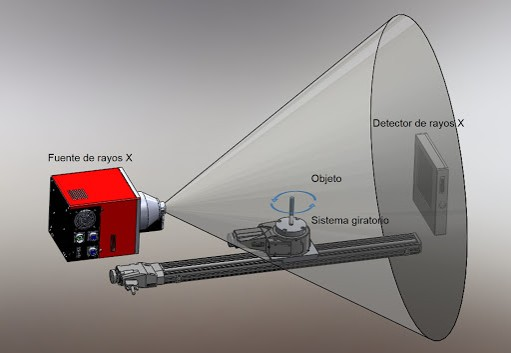
\includegraphics[width=0.5\textwidth]{images/esquema_microtomografo.jpg}
    \caption{Esquema de un sistema de microtomografía}
    \label{fig:esquema_tomografo}
\end{figure}

\section{Aparato Experimental: Microtomógrafo}

\subsection{Hardware}

Antes de entrar en detalle en el proceso de calibración, es esencial describir el
microtomógrafo sobre el que se realizó la totalidad de este trabajo. El mismo
forma parte del equipamiento del Laboratorio de Análisis de Materiales por 
Espectrometría de Rayos X (LAMARX), ubicado en la Facultad de Matemática, Astronomía,
Física y Computación de la Universidad Nacional de Córdoba (FAMAF-UNC). Se trata
de un equipo no comercial, ensamblado in situ, y cuenta con los siguientes
componentes:

\begin{enumerate}[label=\alph*)]
    \item Fuente de Rayos X: con un voltaje operacional en el rango 20-90 keV, una
    corriente de 10-200 $\mu$A (con un output máximo de 8 W). Posee un blanco de
    tungsteno y un tamaño de foco de 7 $\mu$m (5$\mu$m a 4 W); una ventana de berilio
    de 150 $\mu$m a una distancia de 9.5 mm del foco. El cono de rayos X emitido
    tiene un ángulo de apertura de 39$^{\circ}$ \cite{manual_fuente}.
    \item Detector Teledyne DALSA Shad-o-Box 6K HS, con centellador: con un área activa de $11.4\times
    14.6\text{ cm}^2$ (2304$\times$2940 pixeles), una resolución $\Delta p= 49.5\mu\text{m}$
    (tamaño de pixel) y un frame rate de 15 fps \cite{manual_detector}.
    \item Porta-muestra: Base de 5 cm de diámetro (intercambiable) con tres grados
    de libertad de movimiento. Movimiento longitudinal a través de un brazo mecánico
    controlado por un micro-motor, rango de $\sim 30$ cm y paso de 0.00635 mm. Movimiento
    vertical a través de un micro-motor, rango de $\sim 5$ cm y paso de 0.1 mm.
    Movimiento rotacional alrededor del eje vertical, a través de un micro-motor,
    rango de 360$^{\circ}$, con pasos de $\sim 0.026$$^{\circ}$. A su vez, el brazo mecánico posee una
    cámara apuntando directamente al porta-muestra, conectada a una computadora.
    \item Caja interna de protección radiológica: formada por paredes de plomo de 5 mm de espesor,
    con un tamaño de $85\times 38\times 48\text{ cm}^3$. Contiene la
    fuente, el porta-muestra y el detector, y sus paredes son desmontables para poder
    operar en su interior.
    \item Caja externa de protección radiológica: Caja con paredes reforzadas con láminas de plomo,
    con un tamaño de $150\times 120\times 100\text{ cm}^3$. Completamente cerrada, con dos
    puertas para acceder a su interior. Contiene todo el aparato en su interior sobre
    una mesa de mármol. Posee sensores en sus puertas que apagan la fuente al ser
    abiertas, si esta estaba en funcionamiento.
\end{enumerate}

En la figura \ref{fig:tomografo}.a se muestra la caja exterior, dentro de la cual está
contenido el microtomógrafo. En la figura \ref{fig:tomografo}.b puede observarse la
disposición del microtomógrafo
previa a este trabajo, donde cada componente está posicionado sobre la mesa de mármol,
independiente uno de otro.
Aunque esto permite una fácil manipulación de cada elemento
individual, presenta en realidad una gran desventaja: el sistema es muy propenso a
desalineaciones accidentales, lo que implicaría la necesidad de una re-calibración. Para evitar esta
situación, uno de los primeros cambios que se implementaron fue fijar la fuente y
el detector sobre una base rígida, diseñada a medida y formada por caños rectangulares
de acero (ver figura \ref{fig:tomografo}.c). Para ello, fue necesario realizar
una serie de operaciones para alinear correctamente ambos elementos, las cuales están
explicadas en detalle en la sección \ref{sec:calibracion_espacial}. De esta forma, la fuente
y el detector quedan siempre fijos en relación al otro, y se elimina una de las posibles
causas de desalineación. Aún así, el porta-muestra permanece independiente del
sistema fuente-detector. La imagen \ref{fig:tomografo}.d muestra la disposición final del
sistema, similar a la de la figura \ref{fig:tomografo}.c pero con el detector rotado 90$^{\circ}$ en
sentido anti-horario. Este cambio se debe a que la mayoría de las muestras que uno estudia
con un microtomógrafo suelen ser más alargadas en su eje principal de simetría (el que se
usa como rotación), por lo que así se aprovecha mejor el área activa del detector, y se
evita el tener que rotar las imágenes.

\begin{figure}[t]
    \centering
    % Primera fila
    \begin{overpic}[width=0.45\linewidth]{images/caja_ext.png}
        \put(2, 65){\colorbox{black!60}{\color{white}\bfseries\large (a)}}
    \end{overpic}\hspace{2ex}
    \begin{overpic}[width=0.45\linewidth]{images/tomografo_antes.jpg}
        \put(2, 65){\colorbox{black!60}{\color{white}\bfseries\large (b)}}
    \end{overpic}
    
    \vspace{2ex} % Espaciado entre filas
    
    % Segunda fila
    \begin{overpic}[width=0.45\linewidth]{images/tomografo_ahora.jpg}
        \put(2, 65){\colorbox{black!60}{\color{white}\bfseries\large (c)}}
    \end{overpic}\hspace{2ex}
    \begin{overpic}[width=0.45\linewidth]{images/sist_final.jpeg}
        \put(2, 65){\colorbox{black!60}{\color{white}\bfseries\large (d)}}
    \end{overpic}
    
    \caption{\textbf{a)} Caja de contención externa, equipada con alarma y apagado automático.
    \textbf{b)} Distribución original del micro-tomógrafo. Todos los elementos están separados
    y son independientes. \textbf{c)} Segunda iteración del micro-tomógrafo. Fuente y detector
    están fijos y alineados sobre una base de metálica. \textbf{d)} Última iteración del sistema.
    Se rotó 90$^{\circ}$ en sentido anti-horario el detector.}
    \label{fig:tomografo}
\end{figure}


Otro cambio realizado fue el diseño de una serie de porta-muestras cilíndricos con láminas
de plástico. Estos sirven para contener objetos suspendidos en algodón, material que es casi transparente
para los rayos X, pudiendo adquirir imágenes de las muestras sin que estas sean
opacadas por la base en la que se ubican.



\subsection{Software}

El software de adquisición de imágenes del microtomógrafo es \textit{Sapera LT} y \textit{CamExpert},
desarrollados ambos por la empresa Teledyne DALSA \cite{manual_detector}. Para controlar los
micro-motores del sistema, y para integrar las rutinas de adquisición, se utilizó un software de control
desarrollado en el laboratorio. Y para la reconstrucción de las tomografías, se utilizó el software
comercial \textit{NRecon} (utilizado por marcas comerciales de microtomógrafo como \textit{Bruker}),
que implementa el algoritmo de retroproyección filtrada
y permite realizar algunas correcciones geométricas previas.

Por otro lado, el principal software utilizado para el análisis y para el procesamiento de
proyecciones y tomografías fue \textit{FIJI-ImageJ} \cite{FIJI}\cite{FIJI2}. Este es un software gratuito
y de código abierto, con una amplia gama de herramientas para la investigación científica
a partir de imágenes digitales, con la capacidad de realizar análisis cuantitativos, operaciones
matemáticas complejas, transformaciones geométricas, segmentación, etc. Además, permite la
creación de \textit{macros} y \textit{plugins} personalizados (los cuales pueden ser compartidos con la comunidad),
lo que lo convierte en una herramienta muy versátil para este trabajo. Para la visualización de las tomografías, se utilizó el software gratuito \textit{3D Slicer} \cite{3DSlicer1}
\cite{3DSlicer2}, también de código abierto y con amplias posibilidades de análisis.

También se utilizó el software \textit{TASMIP} \cite{TASMIP}, para la simulación de espectros
de rayos X emitidos por la fuente, en función del voltaje aplicado, el material del blanco, y
cualquier posible filtro utilizado. Este software provee una simulación lejos de ser exacta,
pero que permite obtener una aproximación general de la distribución de energía del haz.

Por último, para el análisis y procesamiento de datos y resultados, se implementaron códigos
personalizados en Python.

\section{Desalineaciones del sistema}

Todos los componentes del sistema deben estar alineados sobre un mismo eje, denominado el \textit{eje
de magnificación}, o eje $\mathcal{M}$ (ver figura \ref{fig:sist_coord}.a). Este coincide con el eje
principal del cono de rayos X emitidos por la fuente y es normal al plano $\mathcal{D}$ de la
pantalla del detector. Para este trabajo, se definen los siguientes sistemas de
coordenadas. El sistema de coordenadas del mundo, con origen en el foco de la fuente, y ejes $X$, $Y$ y $Z$,
donde $X$ coincide con el eje $\mathcal{M}$, $Y$ es paralelo al plano $\mathcal{D}$ y $Z$
es perpendicular a ambos (hacia arriba). El sistema de coordenadas del detector, cuyos ejes $U$, $V$
son paralelos a la cuadrícula de pixeles del detector, y $W$ paralelo a $X$; y su origen se encuentra en su centro geométrico.
El sistema de coordenadas del porta-muestra, con origen en el eje rotación, el eje $\hat{Z}$, y ejes
$\hat{X}$ (definido por la dirección del brazo mecánico) e $\hat{Y}$ (perpendicular a ambos).
Por último, el sistema de coordenadas de la cuadrícula de pixeles (propia del detector) con ejes $u$ y $v$
ortogonales a $U$ y $V$, pero no con el mismo sentido ni origen.

Por defecto, el detector debería estar rotado 90$^{\circ}$ en dirección contraria a las agujas del
reloj respecto de lo que se observa en las
figuras \ref{fig:tomografo}.c y \ref{fig:sist_coord}, ya que el origen ``real'' (donde se comienza
a contar la posición de los pixeles) está en la esquina superior derecha (cuadrante $U>0$ y
$V>0$). La posición en la que se encuentra el detector, a pesar de ser ``incorrecta'' inicialmente, no
implica ningún problema para la adquisición, puesto que puede arreglarse fácilmente rotando
todas las imágenes obtenidas 90$^{\circ}$ en la dirección de las agujas del reloj (lo cual puede ser
automatizado mediante un \textit{macro} en FIJI). Esta rotación, al ser de 90$^{\circ}$, no necesita de ninguna
interpolación de pixeles, por lo que la imagen obtenida es esencialmente la misma que la
original. Pero esta transformación corre también el origen y los ejes de coordenadas $(u,v)$ de
la cuadrícula de pixeles, a la esquina superior izquierda ($U<0$ y $V>0$, ver figura
\ref{fig:sist_coord}). Como en todo este trabajo se utilizaron las imágenes rotadas, y no
las imágenes por defecto, se define el sistema de coordenadas $(u,v)$ como el que se observa en la
figura \ref{fig:sist_coord}.b, tal que su relación con los ejes $U$ y $V$ está dada por
$U = u_0 + u$ y $V = v_0 - v$, donde $(u_0,v_0)$ es el centro geométrico del detector en el
sistema $(u,v)$. Solamente para la última modificación del sistema (en la que se rotó el detector),
se utilizó como sistema $U = u - u'_0$ y $V = v'_0 - v$, donde $(u'_0,v'_0)$ es el nuevo centro geométrico
del detector (se sigue trabajando con $(u,v)$ como origen en la esquina superior izquierda de la imagen).

Por otro lado, es importante aclarar que a lo largo de este trabajo se han realizado numerosas
comparaciones entre mediciones en el mundo ``real'' y mediciones a partir de imágenes. Para
no dar lugar a ambigüedades, todas las mediciones de longitud (y por consiguiente área y volumen),
se asumirán con unidades de medida reales, es decir, del Sistema Internacional. Si una distancia $a$ se mide en una imagen,
entonces se tiene la siguiente relación: $a_{real} = M\cdot a_{proy} = M\cdot \Delta p
[\mu\text{m/px}] \cdot a_{img}[\text{px}]$,
donde $\Delta p$ es el ancho/altura de un pixel del detector. En adelante, toda distancia
medida a través de una imagen será entendida como $a_{proy}$ a menos que se especifique de
otra forma. Es decir, se entenderá como la distancia real proyectada sobre el plano $\mathcal{D}$
del detector, y no como una distancia en pixeles.

\begin{figure}[htpb]
    \centering
    \begin{subfigure}{0.58\textwidth}
        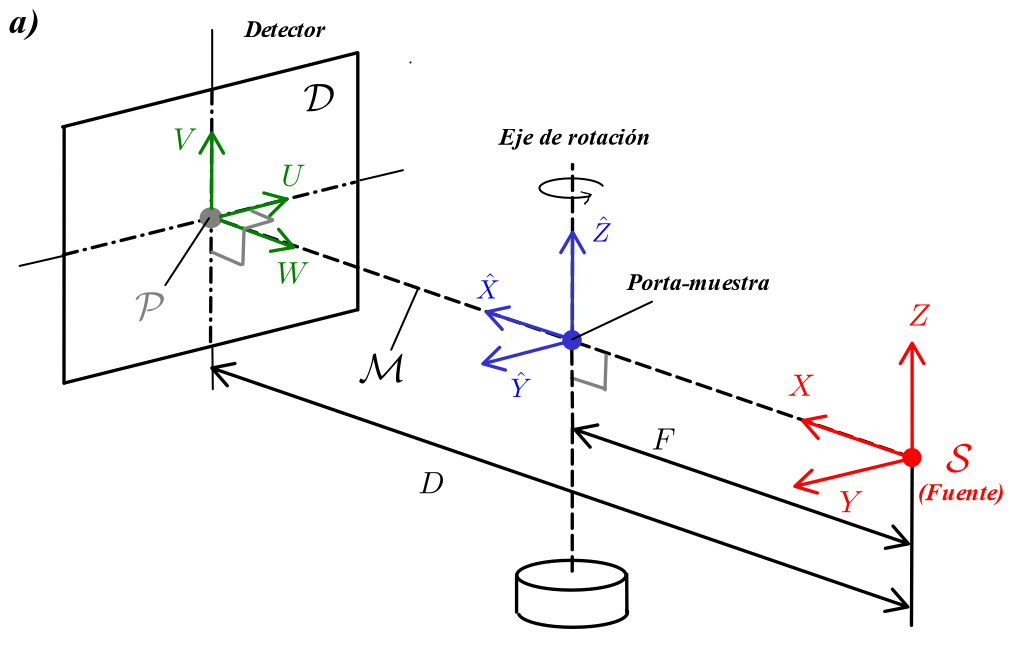
\includegraphics[width=\textwidth]{images/sist_coord1.png}
    \end{subfigure}
    \hfill
    \begin{subfigure}{0.40\textwidth}
        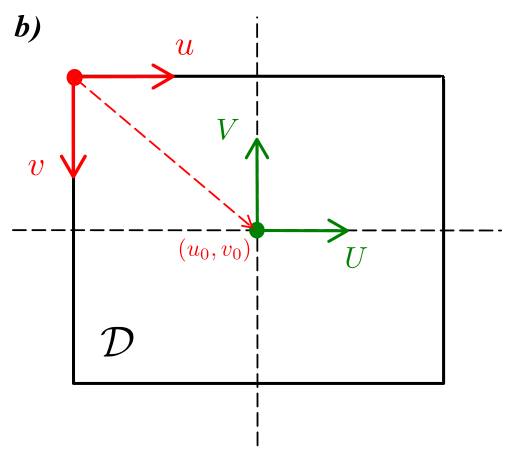
\includegraphics[width=\textwidth]{images/sist_coord2.png}
    \end{subfigure}
    \caption{Sistemas de coordenadas de un sistema de $\mu$CT. \textbf{a)} Representación
    ideal del sistema. El eje de magnificación $\mathcal{M}$ (eje principal del cono de rayos X)
    define los ejes $(X,Y,Z)$ del mundo, con origen en el foco de la fuente ($\mathcal{S}$);
    los ejes $\hat{X}$ del porta-muestra y $W$ del detector están alineados con $\mathcal{M}$;
    el eje $V$ del plano del detector ($\mathcal{D}$) es paralelo, en la misma dirección,
    que el eje de rotación de la muestra, $\hat{Z}$; el punto principal $\mathcal{P}$ se
    encuentra en el centro geométrico del detector; $\mathcal{P}$ y el porta-muestra están a
    distancias $D$ y $F$ del foco, respectivamente. \textbf{b)} Sistema de coordenadas propio
    de la imagen obtenida por el detector, $(u,v)$ y sistema de coordenadas $(U,V)$ empleado
    para la alineación, con origen en el centro geométrico $(u_0,v_0)$.}
    \label{fig:sist_coord}
\end{figure}

Para obtener una reconstrucción precisa a partir de las proyecciones, el algoritmo de
de retroproyección filtrada asume un sistema con una serie de características ideales.
Se define una desalineación como \textit{cualquier desviación geométrica del sistema
ideal que produce un artefacto}, también llamada comunmente en la literatura \textit{factor
de influencia}. Cada tipo de desalineación tiene un parámetro
geométrico $\zeta$ asociado, tal que $\zeta = 0$ corresponde a un estado ideal
del sistema. A continuación, se detallan las características de un sistema ideal,
así como sus posibles desalineaciones y parámetros geométricos correspondientes
\cite{Sun2006}\cite{Ferrucci2015}\cite{Yang2006}.

\begin{enumerate}[label=\alph*)]
    \item La intersección del eje $\mathcal{M}$ con el plano $\mathcal{D}$, llamado
    \textit{punto principal} $\mathcal{P}$ se encuentra en el centro geométrico
    del detector. El sistema está desalineado si $\mathcal{P}=(\Delta U, \Delta V)$.
    \item El eje $\mathcal{M}$ incide normalmente sobre el plano $\mathcal{D}$. El
    sistema está desalineado si existe alguna inclinación en las dos direcciones
    posibles, y los parámetros geométricos asociados son los ángulos $\theta$ y $\phi$
    (también llamados ángulos ``fuera de plano'').
    \item El eje $\hat{X}$ del porta-muestra coincide con el eje $\mathcal{M}$
    El sistema está desalineado si el eje $\hat{X}$ forma un ángulo $\psi$ con el 
    eje $\mathcal{M}$, o si está desplazado una distancia $\Delta \hat{Y}$ respecto
    de este.
    \item El eje $\hat{Z}$ de rotación del porta-muestra es paralelo al plano $\mathcal{D}$.
    El sistema está desalineado si el eje $\hat{Z}$ forma un ángulo $\vartheta$ con el plano
    $\mathcal{D}$.
    \item El eje $\hat{Z}$ es paralelo al eje $V$ del detector. El sistema está desalineado
    si el eje $\hat{Z}$ forma un ángulo $\eta$ con el eje $V$ (rotación del sistema $(U,V)$
    en el plano $\mathcal{D}$).
    \item El sistema tiene una magnificación $M$ definida por las distancias $D$
    (fuente-detector) y $F$ (fuente-objeto) como indica la ec. \ref{eq:magnificacion}.
    El sistema está desalineado si $M$ no es la esperada, es decir, si existen errores
    $\Delta D$ o $\Delta F$ en la determinación de estas distancias. 

\end{enumerate}

\section{Calibración espacial} \label{sec:calibracion_espacial}

Los parámetros geométricos del sistema son $\{\Delta U, \Delta V, \theta,
\phi, \psi, \Delta \hat{Y}, \vartheta, \eta, \Delta D, \Delta F\}$. El objetivo de la
calibración espacial es reducir o determinar cada uno de estos parámetros
para obtener proyecciones lo más fieles posibles a la realidad, de forma tal que las
mediciones espaciales (distancias, ángulos, etc.) sean lo más precisas posibles. Se
lleva a cabo en dos etapas: una alineación directa del sistema (hardware) por medio
de un ajuste físico de los componentes y una calibración fina, dada por la determinación de
los parámetros geométricos restantes, para una posterior corrección de las proyecciones
(software). Dispositivos comerciales como los de Bruker también tienen sus propios
métodos y software de calibración, a pesar de ya estar ensamblados y supuestamente bien
alineados, y en general estos están basados en principios que se detallan a continuación.

\subsection{Alineación del sistema}

Una primera alineación óptima del sistema reduce drásticamente la cantidad de correcciones
a realizar en el procesamiento de las proyecciones. Para ello, se diseñó y planificó el
siguiente procedimiento.

En primer lugar, se buscó alinear la fuente y el detector para fijarlos sobre la base
rígida, es decir, se trataron los casos a) y b) de la sección anterior. Inicialmente se utilizó
un nivel óptico y un nivel láser para buscar que los componentes sean lo más paralelos posible
a la superficie. Posteriormente, se
estudió la proyección del cono sobre el detector a una distancia cercana y lejana a la
fuente (sin ninguna muestra). La imagen proyectada es, esencialmente, la intersección de
un cono con el plano $\mathcal{D}$, luego esta toma la forma de un círculo si el plano
es perpendicular al eje principal del cono (el eje $\mathcal{M}$), o una elipse si 
existe alguna inclinación fuera de plano. Rotando muy de a poco el detector, 
se pueden reducir los ángulos $\theta$ y $\phi$. 
Por otro lado, para hacer coincidir el punto principal $\mathcal{P}$
con el centro del detector, se ajustó manualmente la posición de este con respecto a la
fuente hasta acercar ambos puntos lo máximo posible. Una vez se hicieron ambas cosas,
se alejó el detector a una distancia tal que el círculo proyectado ocupaba casi toda
la pantalla, y se repitió todo el procedimiento anterior. De esta forma, iterando varias
veces entre ambas posiciones del detector, es posible reducir los parámetros $\Delta U$,
$\Delta V$, $\theta$ y $\phi$ (ver figura \ref{fig:alineacion_fuente}). Para todo este
procedimiento, se diseñó un \textit{macro} en FIJI, capaz de binarizar la imagen, hallar los centros
de las figuras y calcular los criterios de similitud presentados en la ec. \ref{eq:circ_R},
para facilitar el trabajo y el análisis. El mismo está adjunto en el Apéndice B.1.

Es importante destacar que la posición final del detector es más alejada que cualquiera
de las posiciones utilizadas para la alineación, ya que el cono de rayos X debe llegar
a cubrir toda la pantalla. Es decir, una vez encontradas la dirección y orientación
correctas, a partir del método anterior, se aleja el detector una distancia adecuada,
con cuidado de mantenerlo en la misma línea imaginaria (eje $\mathcal{M}$). 

\begin{figure}[htpb]
    \centering
    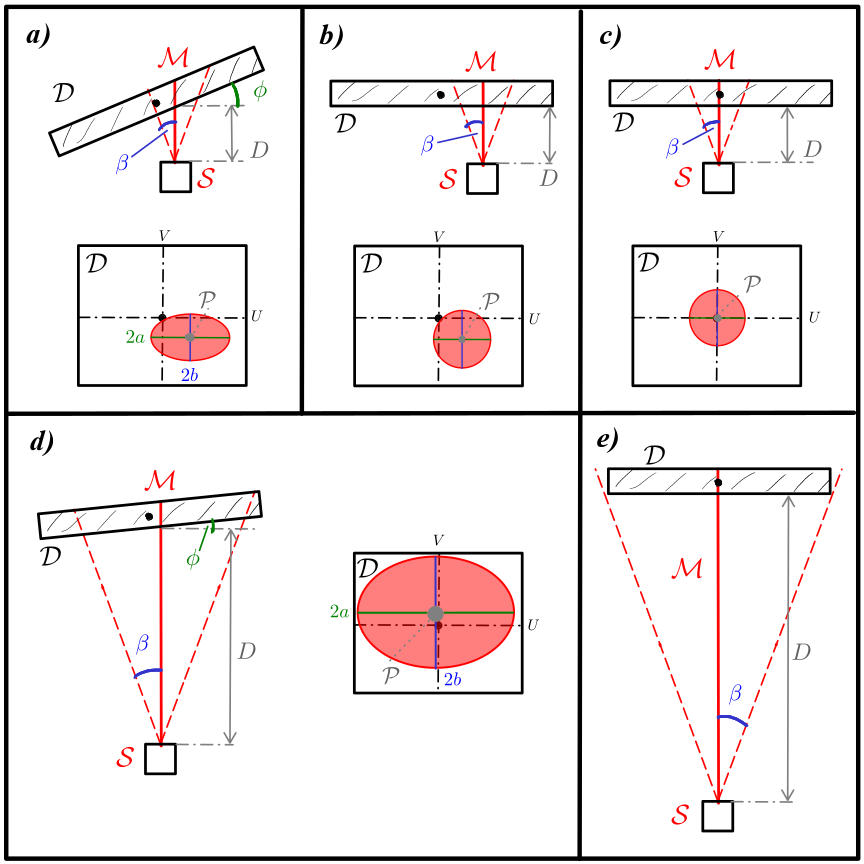
\includegraphics[width=\textwidth]{images/alineacion_fuente.png}
    \caption{Proceso de alineación fuente-detector (visto desde ``arriba''). \textbf{a)} Detector
    inicialmente desalineado, con inclinación y desplazamiento (en este caso, solo inclinación $\phi$
    alrededor de $V$, y desplazamiento en $Y$ y $Z$) con respecto a la fuente y al eje $\mathcal{M}$.
    La proyección del cono será una elipse desplazada del centro. \textbf{b)} Tras rotar correctamente
    el detector hasta colocarlo paralelo al eje $\mathcal{M}$, la elipse proyectada se convierte
    en un círculo. \textbf{c)} Manteniendo la orientación, se desplaza vertical y horizontalmente
    el detector, hasta lograr que el punto principal $\mathcal{P}$ coincida con el centro de la
    pantalla. \textbf{d)} Se aleja el detector a una distancia intermedia, y se repite el procedimiento
    anterior. Posteriormente, se verifica que en la primera distancia siga estando alineado. \textbf{e)}
    Una vez que el detector se encuentra alineado en todo el trayecto evaluado, se lo lleva a
    su posición final, lo suficientemente alejado como para que la proyección del cono apenas supere
    toda la pantalla.}
    \label{fig:alineacion_fuente}
\end{figure}

Una vez fijos la fuente y el detector, se procedió a alinear el porta-muestra, específicamente
los casos c) y e) de la sección anterior. Para esto, se colocó un objeto cilíndrico y alargado
en la dirección vertical, y se realizó un procedimiento similar al anterior (distancias cercana $x_1$
y lejana $x_2$ a la fuente). En cada posición, se tomaron dos proyecciones, una de ellas con 
el porta-muestra rotado 180$^{\circ}$ con respecto a la otra. Reflejando esta última imagen (en el eje
vertical) y superponiéndola a la primera, se puede estudiar la alineación del porta-muestra.
Si las imágenes se superponen perfectamente en el centro, el porta-muestra está sobre el eje
$\mathcal{M}$ (a esa distancia $x_i$ específica), de lo contrario se observa una superposición
parcial o nula de los cilindros. La alineación se realiza comparando esta misma situación en las
dos distancias. Si en las dos sucede que al superponer las imágenes los cilindros
están separados, quiere decir que en ninguna posición intermedia el eje $\hat{X}$ interseca con
el eje $\mathcal{M}$, por lo que debe desplazarse todo el sistema de forma paralela. Una vez
se observa que en alguna distancia ocurre una superposición de los cilindros, se sabe que en ese
punto (o alguno cercano) se da la coincidencia de los ejes. Queda entonces inclinar levemente
el eje $\hat{X}$, hasta que la coincidencia ocurra también en el otro extremo $x_j$.
Después de múltiples iteraciones de este proceso, revisando en ambas distancias, se puede reducir
cada vez más la distancia y el ángulo entre los ejes, hasta obtener que los cilindros se superponen
completamente en ambas distancias. Para ello, se diseñó un \textit{macro} en FIJI que automatiza el proceso
(ver Apéndice B.2).

En la figura \ref{fig:alineacion_muestra} se observa con mayor detalle el proceso, y cómo la
inclinación y distancia entre los ejes se relaciona con la posición de los cilindros en las
imágenes superpuestas (una normal y la otra reflejada). En particular, se puede conocer (o
al menos aproximar) la distancia $d$ a la que se encuentra el eje $\hat{X}$ del eje $\mathcal{M}$
($d$ un segmento perpendicular a $\mathcal{M}$), en alguno de los puntos $x_i$, estudiando la
separación entre los centros de los cilindros $\Delta x_i$ en la superposición de imágenes.
Conociendo el diámetro real del cilindro, $\mathsf{D}_{real}$, y midiendo el diámetro magnificado en la imagen,
$\mathsf{D}_{mag}$, se puede calcular la magnificación $M(x_i)$. Así, se tiene

\begin{equation}
    d_i = \frac{\Delta d_i}{2M} = \frac{\Delta d_i}{2} \frac{\mathsf{D}_{real}}{\mathsf{D}_{mag}}
    \label{eq:alineacion_muestra}
\end{equation}


\begin{figure}[htpb]
    
    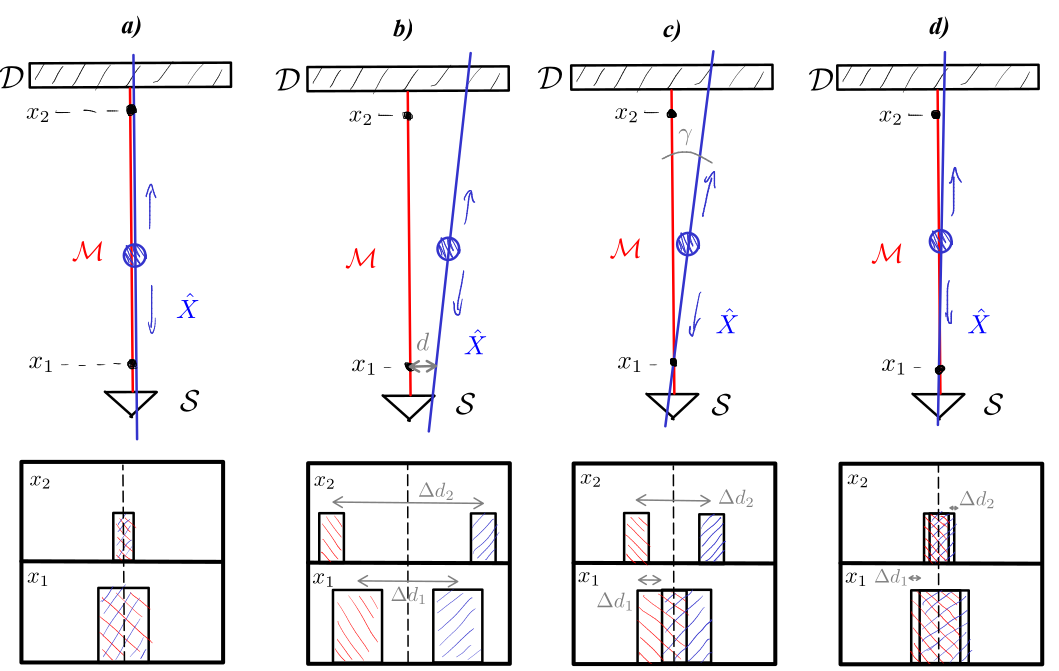
\includegraphics[width=\textwidth]{images/alineacion_muestra.png}
    \caption{Alineación del sistema fuente-detector (eje $\mathcal{M}$) con el eje de movimiento
    de la muestra (eje $\hat{X}$). Arriba se observa la posición de cada elemento del sistema, así
    como las distancias cercana y lejana a la fuente ($\mathcal{S}$), $x_1$ y $x_2$ respectivamente.
    Abajo se observan las imágenes superpuestas de los cilindros (rojo ``real'', y azul
    ``reflejada''), para cada distancia $x_i$. \textbf{a)} Estado ideal del sistema, con ambos
    ejes perfectamente alineados, y los cilindros completamente superpuestos en ambas distancias.
    \textbf{b)} Desalineación arbitraria del sistema, con el eje $\hat{X}$ desplazado e inclinado
    respecto a $\mathcal{M}$; en las dos distancias los cilindros se encuentran completamente
    separados. \textbf{c)} Intersección de los ejes en un punto cercano a $x_1$; superposición
    parcial de los cilindros en $x_1$. \textbf{d)} Reducción de la separación entre ejes; superposición casi
    completa de los cilindros, en ambas distancias.}
    \label{fig:alineacion_muestra}
\end{figure}

En realidad, aunque ambos ejes estén perfectamente alineados, puede suceder que los cilindros no
se superpongan perfectamente. Esto se debe al caso \textbf{e)} de las desalineaciones presentadas,
una inclinación $\eta$, en el plano $\mathcal{P}$, entre los ejes $V$ y $\hat{Z}$ (eje de rotación).
Este ángulo se puede aproximar a través de la misma superposición de los cilindros (real y reflejado).
Para ello, se trazan los ejes principales de cada cilindro, y se mide el ángulo entre ellos. Si
$\eta=0$, los ejes están perfectamente superpuestos y no hay ángulo. Si el cilindro está inclinado
hacia el eje $\hat{Y}$ a causa del porta-muestra, entonces su reflexión se verá inclinada hacia el
otro lado, el mismo ángulo. Por lo tanto, el ángulo medido entre los dos ejes proyectados es $2\eta$
(ver figura \ref{fig:alineacion_eta}).

\begin{figure}[htpb]
    \centering
    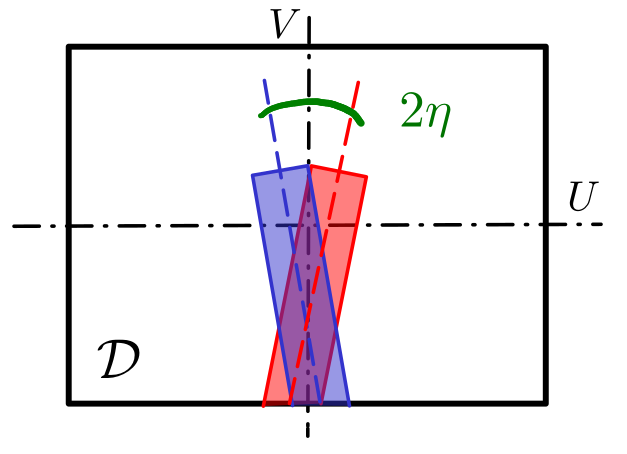
\includegraphics[width=0.4\textwidth]{images/alineacion_eta.png}
    \caption{Determinación de la inclinación $\eta$ (en el plano $\mathcal{D}$) a través de la
    superposición de la proyección de una muestra cilíndrica recta, y su reflexión tras rotarla
    180$^{\circ}$.}
    \label{fig:alineacion_eta}
\end{figure}

Hasta ahora, estos métodos requieren de una constante intervención y manipulación del hardware: movimiento,
inclinación y ajuste de todas las piezas involucradas. Y aunque las mejoras obtenidas en la reconstrucción
pueden ser drásticas, son limitadas por la destreza del operario y los instrumentos que tenga a su
disposición. A continuación, se mostrará un método de determinación de parámetros de forma analítica.

\subsubsection{Determinación de correcciones finas}

Existen numerosos métodos basados en la derivación analítica de las expresiones matemáticas
que relacionan mediciones obtenidas con los distintos factores de influencia, bajo un marco
o modelo de medición (en este caso, de un sistema de haz cónico) \cite{Ferrucci2015}.
Muchos de estos utilizan objetos de referencia (comúnmente llamados \textit{fantomas}), cuya
geometría es bien conocida, para extraer información de las proyecciones. En particular, muchos
de los métodos existentes para determinar los parámetros geométricos mencionados
utilizan fantomas que contienen esferas pequeñas y de alta densidad (o alta atenuación), que
funcionan como \textit{puntos marcadores} de coordenadas en las imágenes proyectadas, para obtener
mediciones precisas. A continuación se detallan dos métodos en particular, uno basado en una rotación
ideal del porta-muestra (es decir, requiere proyecciones de múltiples ángulos), y otro basado en
una posición fija del porta-muestra.

\medskip
\textit{A.Método de múltiples proyecciones.}
\smallskip

Si se considera un sistema cuyo porta-muestra rota de forma ideal (el eje $\hat{Z}$ permanece siempre
fijo), entonces un punto marcador ubicado fuera del eje de rotación recorrerá una trayectoria
circular. En un sistema de haz cónico, dicha trayectoria se proyecta sobre el plano del detector
como una elipse o una línea recta (en el caso específico en que la esfera gira sobre un plano que
contenga el eje $\mathcal{M}$). Aprovechando este hecho, se han diseñado múltiples fantomas
alrededor del mismo principio: el análisis geométrico de elipses proyectadas en el detector,
a partir de varios puntos marcadores (esferas pequeñas o ``ball bearings'' - BB's) rotando. \cite{Ferrucci2015} \cite{Noo2000}.
El método detallado a continuación fue desarrollado por Yang \textit{et al.} \cite{Yang2006}, y sirve
para determinar los parámetros {$\Delta U, \Delta V, \eta, D, F$}, mediante técnicas de regresión
lineal.

Para este análisis, se asume que las inclinaciones fuera del plano $\mathcal{D}$ ($\theta$ y
$\phi$) son despreciables, es decir, menores a 5$^{\circ}$. Esto es posible gracias a la observación
experimental de von Smekal \textit{et al.} \cite{Smekal2004} y su posterior demostración analítica por
Yang \textit{et al.} \cite{Yang2006}. Esto es, las distorsiones en la imagen provocadas por estas desviaciones
son mínimas; en concreto, para un haz cónico con semi-ángulo de apertura $\beta=20$$^{\circ}$, el error
porcentual en la posición proyectada de un punto marcador es menor al $4\%$ (y este valor es
alcanzado solo en los bordes de la pantalla, lejos del centro del cono), como se observa en los gráficos
de la figura \ref{fig:graf_yang1}.

\begin{figure}[htpb]
    \centering
    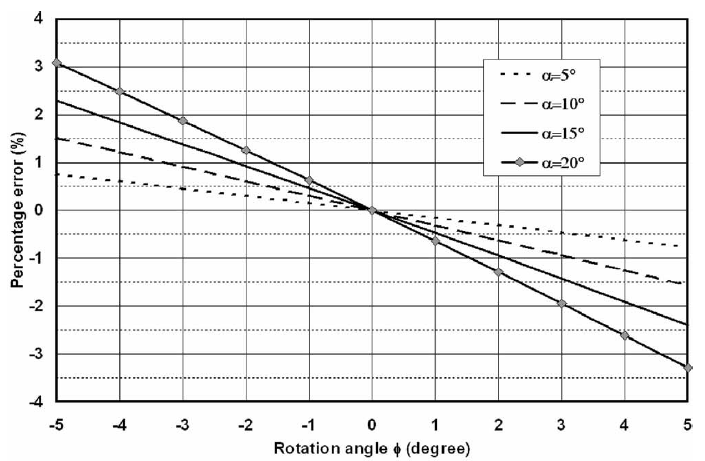
\includegraphics[width=0.65\textwidth]{images/graf_yang1.png}
    \caption{Error relativo de la posición proyectada de un punto marcador (respecto a la posición
    ideal) en función del ángulo fuera de plano $\phi$ (el caso es análogo para $\theta$), para un haz cónico de
    apertura $2\alpha$ ($2\beta$ en este trabajo). Gráfico extraído de Yang \textit{et al.} \cite{Yang2006}.}
    \label{fig:graf_yang1}
\end{figure}

Como fantoma, se utiliza un cilindro vertical de algún material de baja atenuación, con una serie
de esferas metálicas como puntos marcadores, alineadas verticalmente en la superficie del cilindro
(ver figura \ref{fig:metodo_yang}.a).
No es estrictamente necesario que sean equidistantes, pero resulta conveniente. Para cada marcador
$i$, se identifican en su trayectoria elíptica cinco puntos de referencia $\vec{p}_{ij} = (u_{ij},v_{ij})$
($0 \leq j\leq 4$). $j=0$ corresponde al centro geométrico de la elipse, mientras que $j=1,2,3,4$ 
están determinados a partir de las distancias máximas y mínimas entre "pares radiales" (puntos
desfasados 180$^{\circ}$ en la rotación), que coinciden con los cuatro vértices de la elipse proyectada
(ver figura \ref{fig:metodo_yang}.b).
A partir de las coordenadas obtenidas, se definen las siguientes variables:

\begin{equation}
    \left\{
    \begin{aligned}
        x_i &= sgn(v_{i0} - v_0)\frac{v_{i3} - v_{i1}}{|\vec{p}_{i2} - \vec{p}_{i4}|}\\
        y_i &= \frac{v_{i3} + v_{i1}}{2}    
    \end{aligned}
    \right.
    \hspace{15mm}
    sgn(x)=
    \left\{
    \begin{aligned}
        -1 \hspace{5mm}& x<0\\
        1 \hspace{5mm}& x \geqslant 0
    \end{aligned}
    \right.
    \label{eq:variables_yang1}
\end{equation}

Como se demuestra en Yang \textit{et al.} \cite{Yang2006}, se puede ajustar los pares $(x_i,y_i)$ a
una función lineal $y = \mathsf{a_1} + \mathsf{b_1}\cdot x$, tal que 

\begin{equation}
    D = \mathsf{a_1} \hspace{15mm} (v_0 + \Delta V) = \mathsf{b_1}
    \label{eq:Delta_V_D}
\end{equation}

Donde $(u_0, v_0)$ es el centro
geométrico del detector. La razón de utilizar la función $sgn(v_{i0}-v_0)$ en la definición
de $x_i$ se debe a la interpretación de esta misma. $x_i$ es una cantidad cuyo módulo es lineal con
la longitud del eje menor de la elipse. $x_i$ comienza siendo negativo, para elipses ubicadas cerca de
$v=0$, y crece a medida que se acercan al centro; si la elipse está justo en el centro,
$x_i=0$, y a medida que se aleja nuevamente del centro, $x_i$ crece con valores positivos,
manteniendo así la linealidad con $y_i$ para todas las elipses. En realidad, el que define
el cambio de signo no es el centro geométrico, sino el punto principal $(u_0 +\Delta U,
v_0 + \Delta V)$, sin embargo, al ser $\Delta V$ uno de los valores que se desea determinar
con este cambio de variables, se asume que la distancia entre $\mathcal{P}$ y el centro
es lo suficientemente pequeña como para que el ajuste tenga sentido.

Por otro lado, conociendo las coordenadas de los centros de cada elipse, y el valor de
$\Delta V$, puede determinarse los parámetros $\Delta u$ y $\eta$, a partir del siguiente
ajuste lineal $u_{i0} = \mathsf{a_2} + \mathsf{b_2}\cdot v_{i0}$. De esta forma, se obtiene

\begin{equation}
    u_0 + \Delta U = \mathsf{a_2} + \mathsf{b_2}\cdot (v_0 + \Delta V)
    \hspace{15mm}
    \eta = \arctan(\mathsf{b_2})
    \label{eq:delta_u_eta}
\end{equation}

Finalmente, para determinar $F$ se requiere conocer la distancia real $l$ entre dos esferas,
$i=1,2$ (no necesariamente consecutivas), y medir la proyección análoga.

\begin{equation}
    F = \dfrac{l\cdot D}{\sqrt{ (\vec{p}_{10}-\vec{p}_{20})^2 + \left(\frac{\vec{p}_{12} - \vec{p}_{14}}{2}\right)^2
    + \left(\dfrac{\vec{p}_{22} - \vec{p}_{24}}{2}\right)^2 - \dfrac{(\vec{p}_{12} - \vec{p}_{14})(\vec{p}_{22} - \vec{p}_{24})}{2} }}
    \label{eq:F}
\end{equation}

La precisión de este método radica enteramente en la determinación de los puntos $\vec{p}_{ij}$
de cada elipse. Para ello, se comienza obteniendo $N$ proyecciones del cilindro en rotación
(en este trabajo siempre se utilizó $N=352$, aproximadamente una imagen cada desplazamiento
angular de 1$^{\circ}$). Se diseñó un \textit{macro} en FIJI (ver Apéndice B.3) con la tarea de binarizar cada imagen y obtener
las coordenadas de los centros de las esferas metálicas, proyectadas como círculos. A partir
de las $N$ posiciones de cada esfera, $(u_i^{(k)}, v_i^{(k)})$, se determinaron los parámetros
{$A, B, C, u_{i0}, v_{i0}$} de las elipses (ver ec. \ref{eq:elipse}), a través de un ajuste
lineal por cuadrados mínimos detallado por Noo \textit{et al.} \cite{Noo2000}. Diagonalizando la matriz
$\mathbb{A}$ de cada elipse, se calculan los semiejes $a$ y $b$, y se obtienen sus respectivos
autovectores $\mathbf{v_a}$ y $\mathbf{v_b}$. Luego, sabiendo que los puntos $\vec{p}_{ij}$
($j=1,...,4$) son vértices de la elipse, se tiene

\begin{equation}
    \begin{aligned}
        \vec{p}_{i1} &= \vec{p}_{i0} - b_i\cdot \mathbf{v}_{i,b}\\
        \vec{p}_{i2} &= \vec{p}_{i0} - a_i\cdot \mathbf{v}_{i,a}
    \end{aligned}
    \hspace{15mm}
    \begin{aligned}
        \vec{p}_{i3} &= \vec{p}_{i0} + b_i\cdot \mathbf{v}_{i,b}\\
        \vec{p}_{i4} &= \vec{p}_{i0} + a_i\cdot \mathbf{v}_{i,a}
    \end{aligned}
    \label{eq:vertices}
\end{equation}

\begin{figure}[htpb]
    \centering
    \begin{subfigure}{0.28\textwidth}
        \begin{overpic}
            [width=\textwidth]{images/fantom_yang_1.jpg}
            \put(3,85){\colorbox{black!60}{\color{white}\bfseries\large (a)}}
        \end{overpic}        
    \end{subfigure}
    \hfill
    \begin{subfigure}{0.28\textwidth}
        \begin{overpic}
            [width=\textwidth]{images/fantom_yang.jpg}
            \put(3,85){\colorbox{black!60}{\color{white}\bfseries\large (b)}}
        \end{overpic}        
    \end{subfigure}
    \hfill
    \begin{subfigure}{0.42\textwidth}
        \begin{overpic}
            [width=\textwidth]{images/vertices_elipse.png}
            \put(2,60){\colorbox{black!60}{\color{white}\bfseries\large (c)}}
        \end{overpic}        
    \end{subfigure}
    \caption{\textbf{a)} Fantoma utilizado en el método de Yang \textit{et al.} \cite{Yang2006}, con 8
    esferas metálicas como puntos marcadores. \textbf{b)} Fantoma ubicado sobre
    el porta-muestra. \textbf{c)} Proyección de la trayectoria de un punto
    marcador tras una rotación completa; se ajusta una elipse y a partir de los
    parámetros $A$, $B$, $C$, $u_0$ y $v_0$, se determinan los puntos de interés
    $\vec{p}_{ij}$, $j=0,1,2,3,4$.}
    \label{fig:metodo_yang}
\end{figure}

\medskip
\textit{B. Estimación de los ángulos $\theta$ y $\phi$.}
\smallskip

La determinación de los ángulos fuera del plano $\mathcal{D}$ es más complicada y requiere
de métodos más complejos, como análisis de Fourier \cite{Smekal2004} o simulaciones y
optimización numérica \cite{Johnston2008}. Sin embargo, para este trabajo bastará demostrar
que estos son despreciables (<5$^{\circ}$), para que el método de Yang \textit{et al.} \cite{Yang2006} sea aplicable.
Para ello, se propone lo siguiente, teniendo en cuenta el mismo principio que se utilizó en la alineación del sistema 
fuente-detector (ver figura \ref{fig:alineacion_fuente}).

La proyección del cono sobre el detector es una elipse cuando $\theta \neq 0$ o $\phi \neq 0$,
o más en general, cuando el plano $\mathcal{D}$ esté inclinado un ángulo $\alpha$ con respecto
al plano ideal, en cualquier dirección. Conociendo el semi-ángulo $\beta$ de apertura del cono,
y los ejes $a$ y $b$ de la elipse proyectada, es posible determinar $\alpha$ a partir de la
ecuación \ref{eq:alfa_proyeccion}. Utilizando un \textit{macro} en FIJI (Apéndice B.1), se binariza la imagen de
la elipse, y se ajusta sus semi-ejes, para luego determinar $\alpha$. Como $\alpha$ es una
composición de las rotaciones $\theta$ y $\phi$, estos no pueden ser mayores.

Este método es una estimación, ya que se realiza con imágenes en una posición anterior a
la definitiva. El detector, en su estado final, debe estar lo suficientemente alejado de
la fuente como para que el cono ilumine toda la pantalla, siendo imposible verificar su
proyección elíptica. En vez de eso, se mide la elipse de un estado anterior, en la etapa
final de la alineación, y se asume que el desplazamiento hacia la última posición mantiene
la orientación conseguida (lo cual, si no es un sistema mecanizado, depende enteramente
de la destreza del operario). Pero además de aproximar, podría utilizarse el valor de
$\alpha$ y la dirección en la que se inclina (rota alrededor del eje menor), para corregir
las imágenes.

\medskip
\textit{C. Método de única proyección.}
\smallskip

El método propuesto por Sun \textit{et al.} \cite{Sun2006} ofrece una alternativa analítica para la 
calibración geométrica de un sistema de $\mu$CT de haz cónico, con la ventaja distintiva de que
requiere únicamente una proyección de un fantoma de referencia en lugar de múltiples adquisiciones
a diferentes ángulos. Este método utiliza un fantoma de cuatro puntos marcadores (esferas metálicas)
dispuestos en los vértices de un cuadrado de lado $l$ conocido ($l=(35.0 \pm 0.5)$ mm). El objetivo es determinar los siete
parámetros principales de desalineación: $\Delta U$, $\Delta V$, $\eta$, $\theta$, $\phi$, $D$ y $F$.

Los autores llegan a expresiones analíticas que vinculan los parámetros, estudiando todas las
posibles transformaciones geométricas (ver ec. \ref{eq:coord_homog}) de la proyección del cuadrado,
cambiando un factor de influencia a la vez, partiendo de la configuración ideal, y llegando a un
estado de desalineación arbitraria del sistema. Esto es posible, nuevamente, gracias a que la
matriz de transformación $\mathbb{H}$ puede ser obtenida a partir de un producto de transformaciones
$\mathbb{H}_i$ más simples y en un orden específico. Así, los autores demuestran que las
proporciones de los lados del cuadrilátero proyectado en el detector dependen exclusivamente de los
ángulos de rotación y no de los desplazamientos.

El desarrollo matemático es complejo y extenso, por lo que se detalla en el Apéndice A. Sin embargo,
basta con saber que se deben medir las longitudes de los lados del cuadrilátero proyectado ($L_{12}$,
$L_{34}$, $L_{13}$, $L_{24}$), y conocer la longitud real $l$ del lado (ver figura \ref{fig:yisun}).
A partir de las proporciones $L_{12}/L_{34}$ y $L_{13}/L_{24}$, se pueden determinar los ángulos $\theta$
y $\phi$; con estos valores se puede obtener una corrección $\Delta x$ (relacionada con las distancias
$D$ y $F$); y finalmente, analizando la posición de uno de los vértices del cuadrilátero, y con los
valores anteriores, se pueden determinar $\Delta U$, $\Delta V$ y $\eta$.

Este método, además de requerir las mismas condiciones explicadas en los anteriores, asume algunas otras
características. En primer lugar, que el eje $\mathcal{M}$ pasa justo por el centro del cuadrado. Para
ello, se agregó otra esfera metálica también en el centro como ayuda para verificar esto. En segundo
lugar, se asume que el mismo eje de magnificación es perpendicular al plano del cuadrado. Para obtener esto, primero se
lo alineó rotado 90$^{\circ}$ (de perfil), donde es más fácil determinar la orientación correcta estudiando la superposición
de las esferas y del marco de acrílico, y luego se lo rotó 90$^{\circ}$. Posteriormente, se obtuvieron 20 proyecciones
distintas en un rango de 2$^{\circ}$ alrededor de este punto inicial, para determinar la más apropiada.

\begin{figure}[htpb]
    \centering
    \begin{subfigure}{0.45\textwidth}
        \begin{overpic}
            [width=\textwidth]{images/phantom_sun.png}
            \put(3,93){\colorbox{black!60}{\color{white}\bfseries\large (a)}}
        \end{overpic}
    \end{subfigure}
    \hfill
    \begin{subfigure}{0.48\textwidth}
        \begin{overpic}
            [width=\textwidth]{images/cuadrilatero.png}
            \put(3,93){\colorbox{black!60}{\color{white}\bfseries\large (b)}}
        \end{overpic}
    \end{subfigure}
    \caption{\textbf{a)} Fantoma utilizado a partir del método propuesto en Sun \textit{et al.} \cite{Sun2006}.
    \textbf{b)} Cuadrilátero proyectado en el detector para una desalineación arbitraria del sistema. A
    partir de las longitudes de los lados proyectados, las proporciones entre ellos y la longitud real,
    es posible determinar los parámetros geométricos del sistema.}
    \label{fig:yisun}
\end{figure}

\subsection{Resultados}

Se comenzó alineando la fuente y el detector como se indicó anteriormente (ver figura \ref{fig:alineacion_fuente}). La distancia
cercana entre la superficie del detector y el foco de la fuente es $D_1 = (63 \pm 1)$ mm,
y la lejana $D_2 = (133 \pm 1)$ mm (ambas medidas desde el foco hacia la pantalla, con un
medidor láser). Después de múltiples mediciones entre ambas distancias,
realizando pequeños ajustes a la posición horizontal, vertical y orientación de la fuente,
se obtuvieron las proyecciones de la figura \ref{fig:res_alin_fuente} (tras ser umbralizadas).
Utilizando un \textit{macro} (Apéndice B.1),
se ajustaron elipses, y se obtuvieron los parámetros $a$, $b$, $C_W$ y $R$, y se estimaron
los valores de $\Delta U$, $\Delta V$ y $\alpha$ en cada posición. Los valores resultantes
son los mínimos que se pudieron lograr en esta etapa, y posteriormente se trasladó el detector
a su posición final $D = (258 \pm 1)$ mm de la fuente, de tal forma que el cono cubriera toda
la pantalla.

\begin{figure}[htbp]
    \centering
    \begin{subfigure}{0.48\textwidth}
        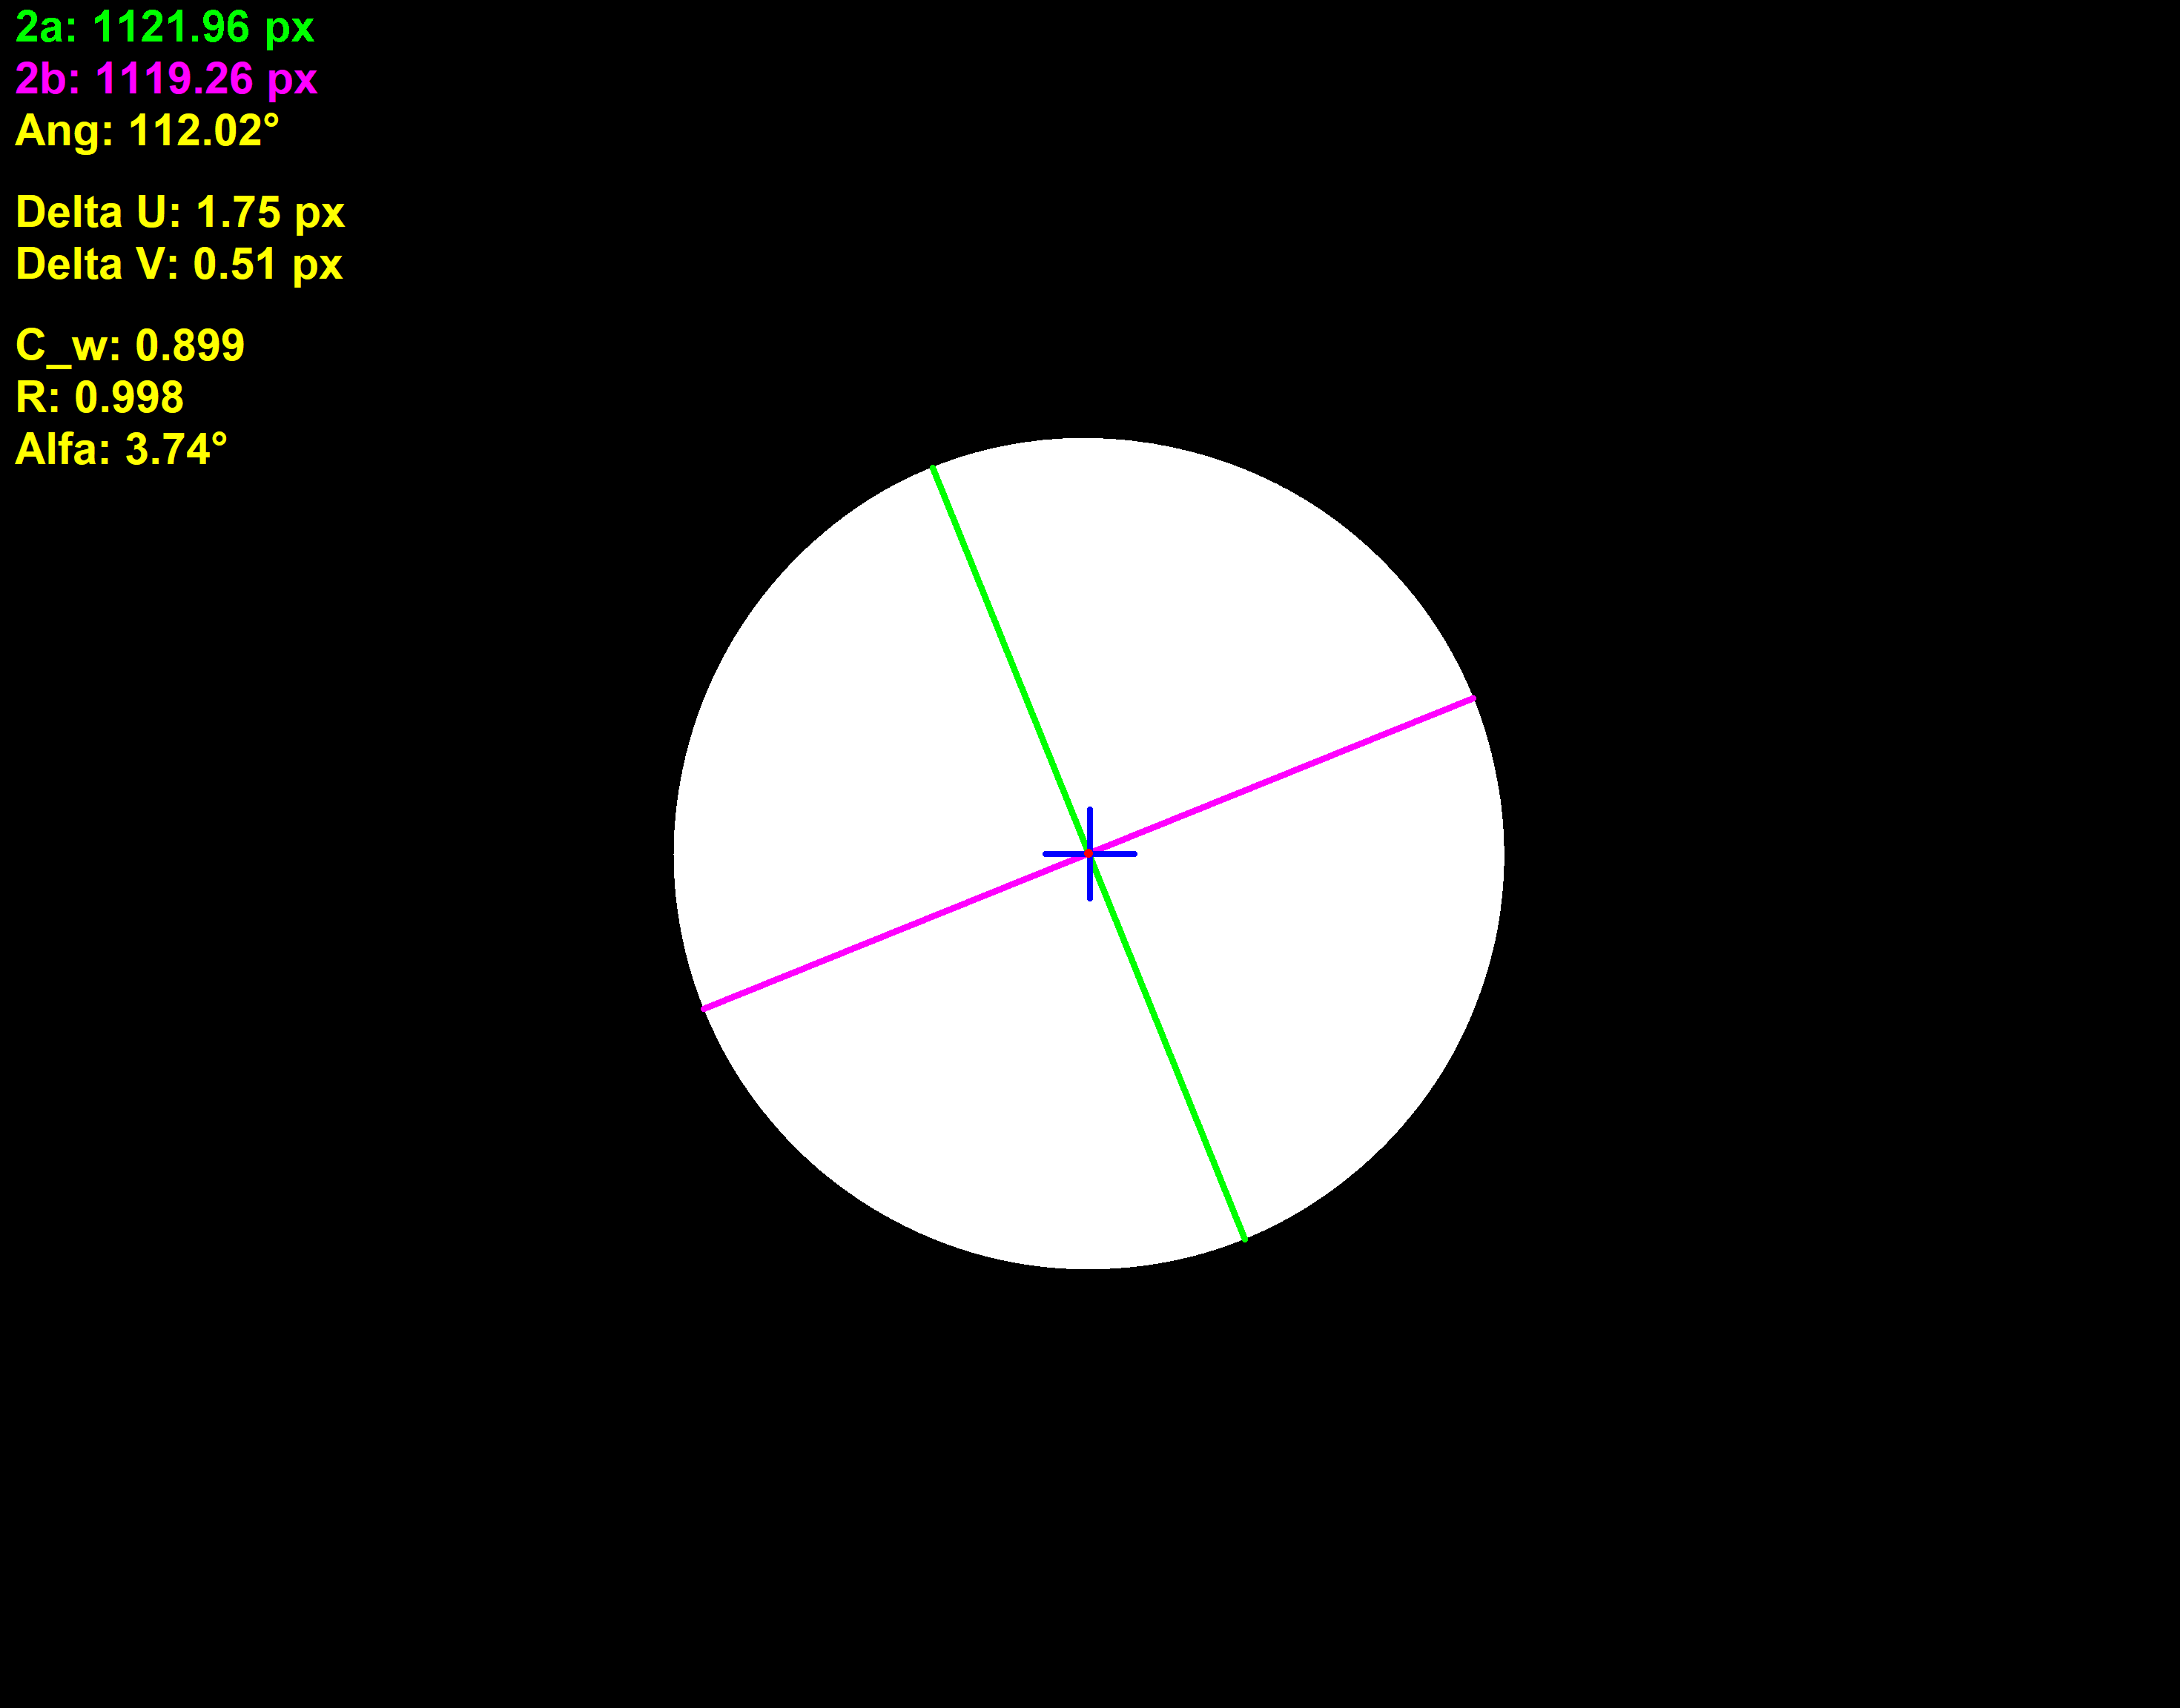
\includegraphics[width=\textwidth]{images/alineacion_cerca.png}
    \end{subfigure}
    \hfill
    \begin{subfigure}{0.48\textwidth}
        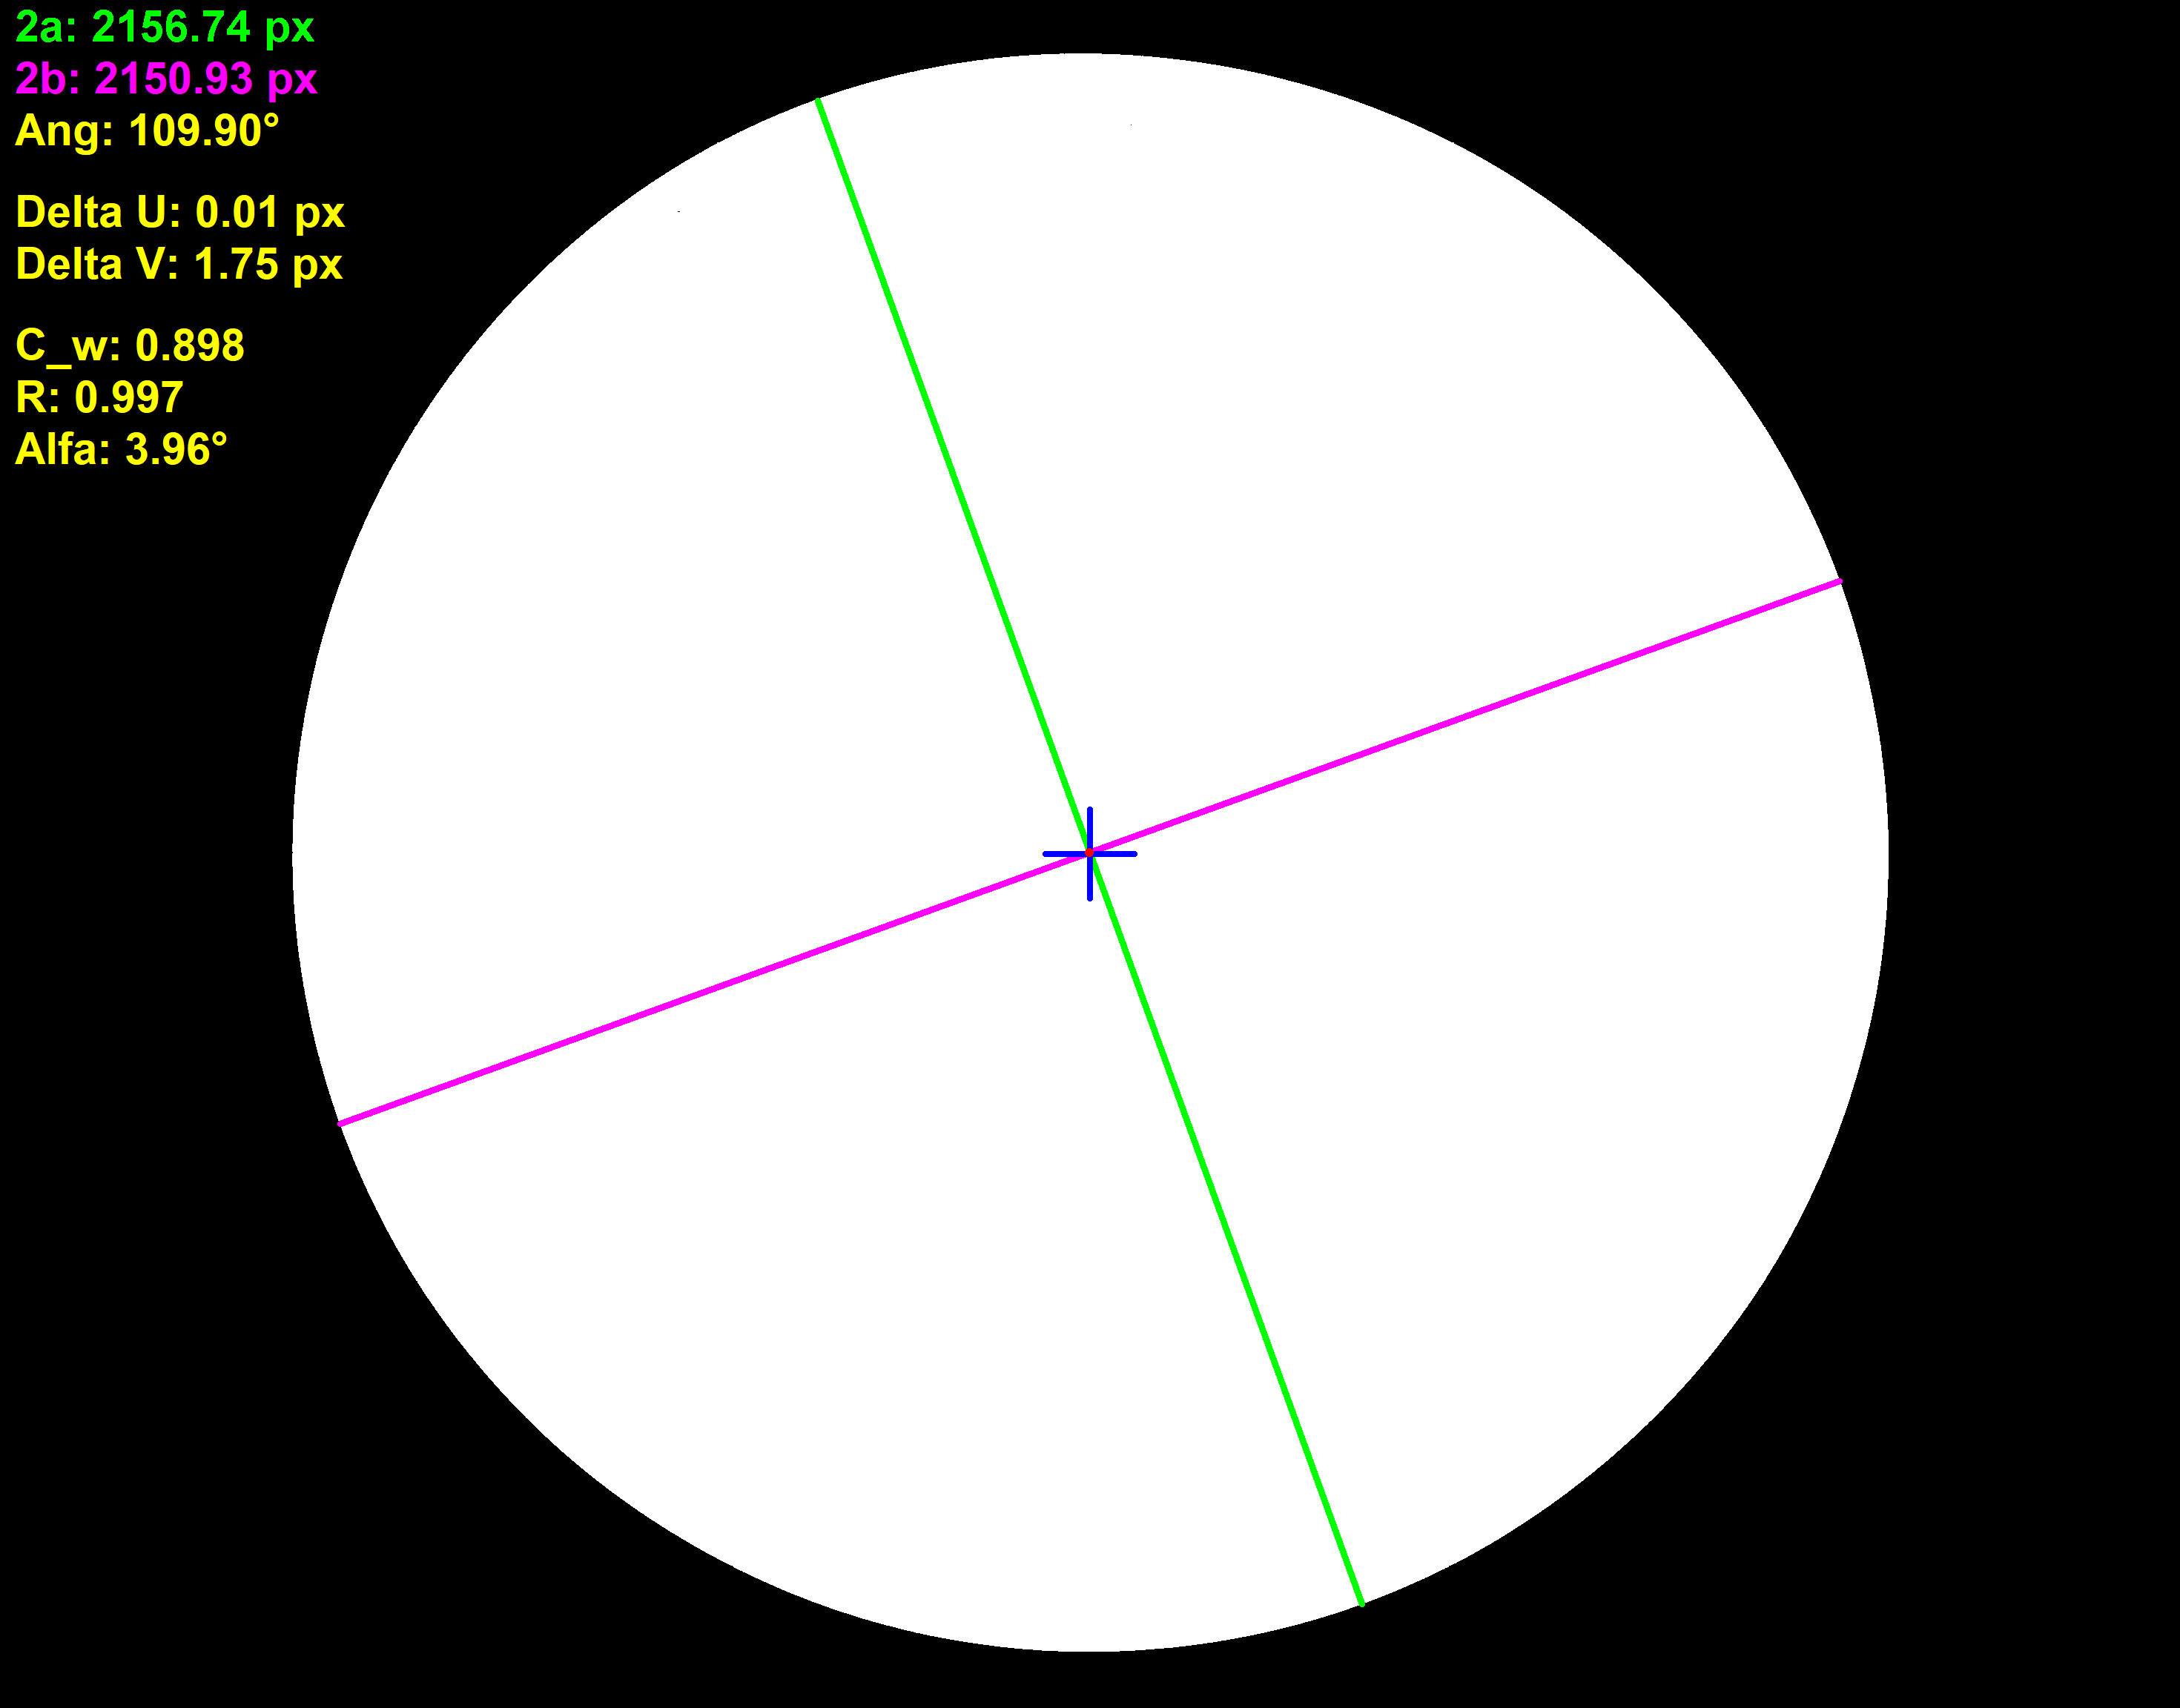
\includegraphics[width=\textwidth]{images/alineacion_lejos.png}
    \end{subfigure}
    \caption{Proyección del cono de rayos X sobre el detector a una distancia $D_1$ cercana
    (\textit{Izq.}) y $D_2$ lejana (\textit{Der.}). Las imágenes están umbralizadas para mostrar
    con mayor claridad, y para poder ajustar las elipses correspondientes, y así, obtener los
    parámetros $a$, $b$, Ang (dirección del eje mayor) $\Delta U$, $\Delta V$, $C_W$, $R$ y $\alpha$.}
    \label{fig:res_alin_fuente}
\end{figure}

Comparando los valores de $\Delta U$ y $\Delta V$ en cada posición, se puede estimar el ángulo $\varPhi$
entre el eje $\mathcal{M}$ y la dirección sobre la que se desplazó el detector a su posición
final. Como dicho desplazamiento se realizó ``a mano'', este ángulo no es una medición precisa,
sino más bien una forma de acotar $\Delta U$ y $\Delta V$ en la posición final (puesto
que no pueden ser medidos como en las posiciones anteriores). Así, se tiene que $\tan(\varPhi_U) \simeq
|\Delta U_1 - \Delta U_2| / |D_1 - D_2|$ y $\tan(\varPhi_V) \simeq |\Delta V_1 - \Delta V_2| / |D_1 - D_2|$,
y se obtiene que estos ángulos son menores a 0.1$^{\circ}$. Por lo tanto, en la posición final $D = (258 \pm 1)$ mm
se espera que $\Delta U, \Delta V < 5$ px. Por otro lado, la desviación del plano $\mathcal{D}$
con respecto al ideal es, en ambas posiciones, menor a 4$^{\circ}$; de la misma manera, se considera
que para la posición final, $\alpha < 4$$^{\circ}$ (cumpliéndose la condición para aplicar el método de múltiples proyecciones).

Fijados fuente y detector, se procedió a alinear el eje de movimiento del porta muestra, como
se indicó anteriormente. Se desplazó el objeto entre dos posiciones, separadas una distancia
$\Delta \hat{x} = (127 \pm 1)$ mm (sistema de coordenadas del eje de rotación). Las imágenes
superpuestas de objeto y su reflejo tras rotar
180$^{\circ}$ en cada posición, se pueden observar en la figura \ref{fig:res_alin_muestra}. Estas fueron
las últimas que se tomaron, tras repetir el proceso numerosas veces y realizar los ajustes
necesarios (como se explicó en la fig. \ref{fig:alineacion_muestra}). Las imágenes fueron umbralizadas
y coloreadas (verde para el objeto en 0$^{\circ}$ y rojo para el objeto en 180$^{\circ}$, y reflejado), para facilitar
el análisis. Con un \textit{macro} (Apéndice B.2), se superpusieron ambas imágenes (el color amarillo representa la región
de superposición entre los dos objetos), y se determinaron los ejes principales de cada objeto, el ángulo $2\eta$
entre ambos, y la distancia $\Delta d$ entre los ejes (medida sobre el eje $U$, es decir, $V=0$). Así, se tiene
que el desplazamiento del eje de rotación respecto al eje $\mathcal{M}$ es $\Delta \hat{y} <
2$ mm (alcanzando este valor solamente muy cerca de la fuente). Por otro lado, se estima que
la inclinación del eje respecto al eje $V$ del detector es $\eta = (0.48 \pm 0.06)$$^{\circ}$.

\begin{figure}[htbp]
    \centering
    \begin{subfigure}{0.49\textwidth}
        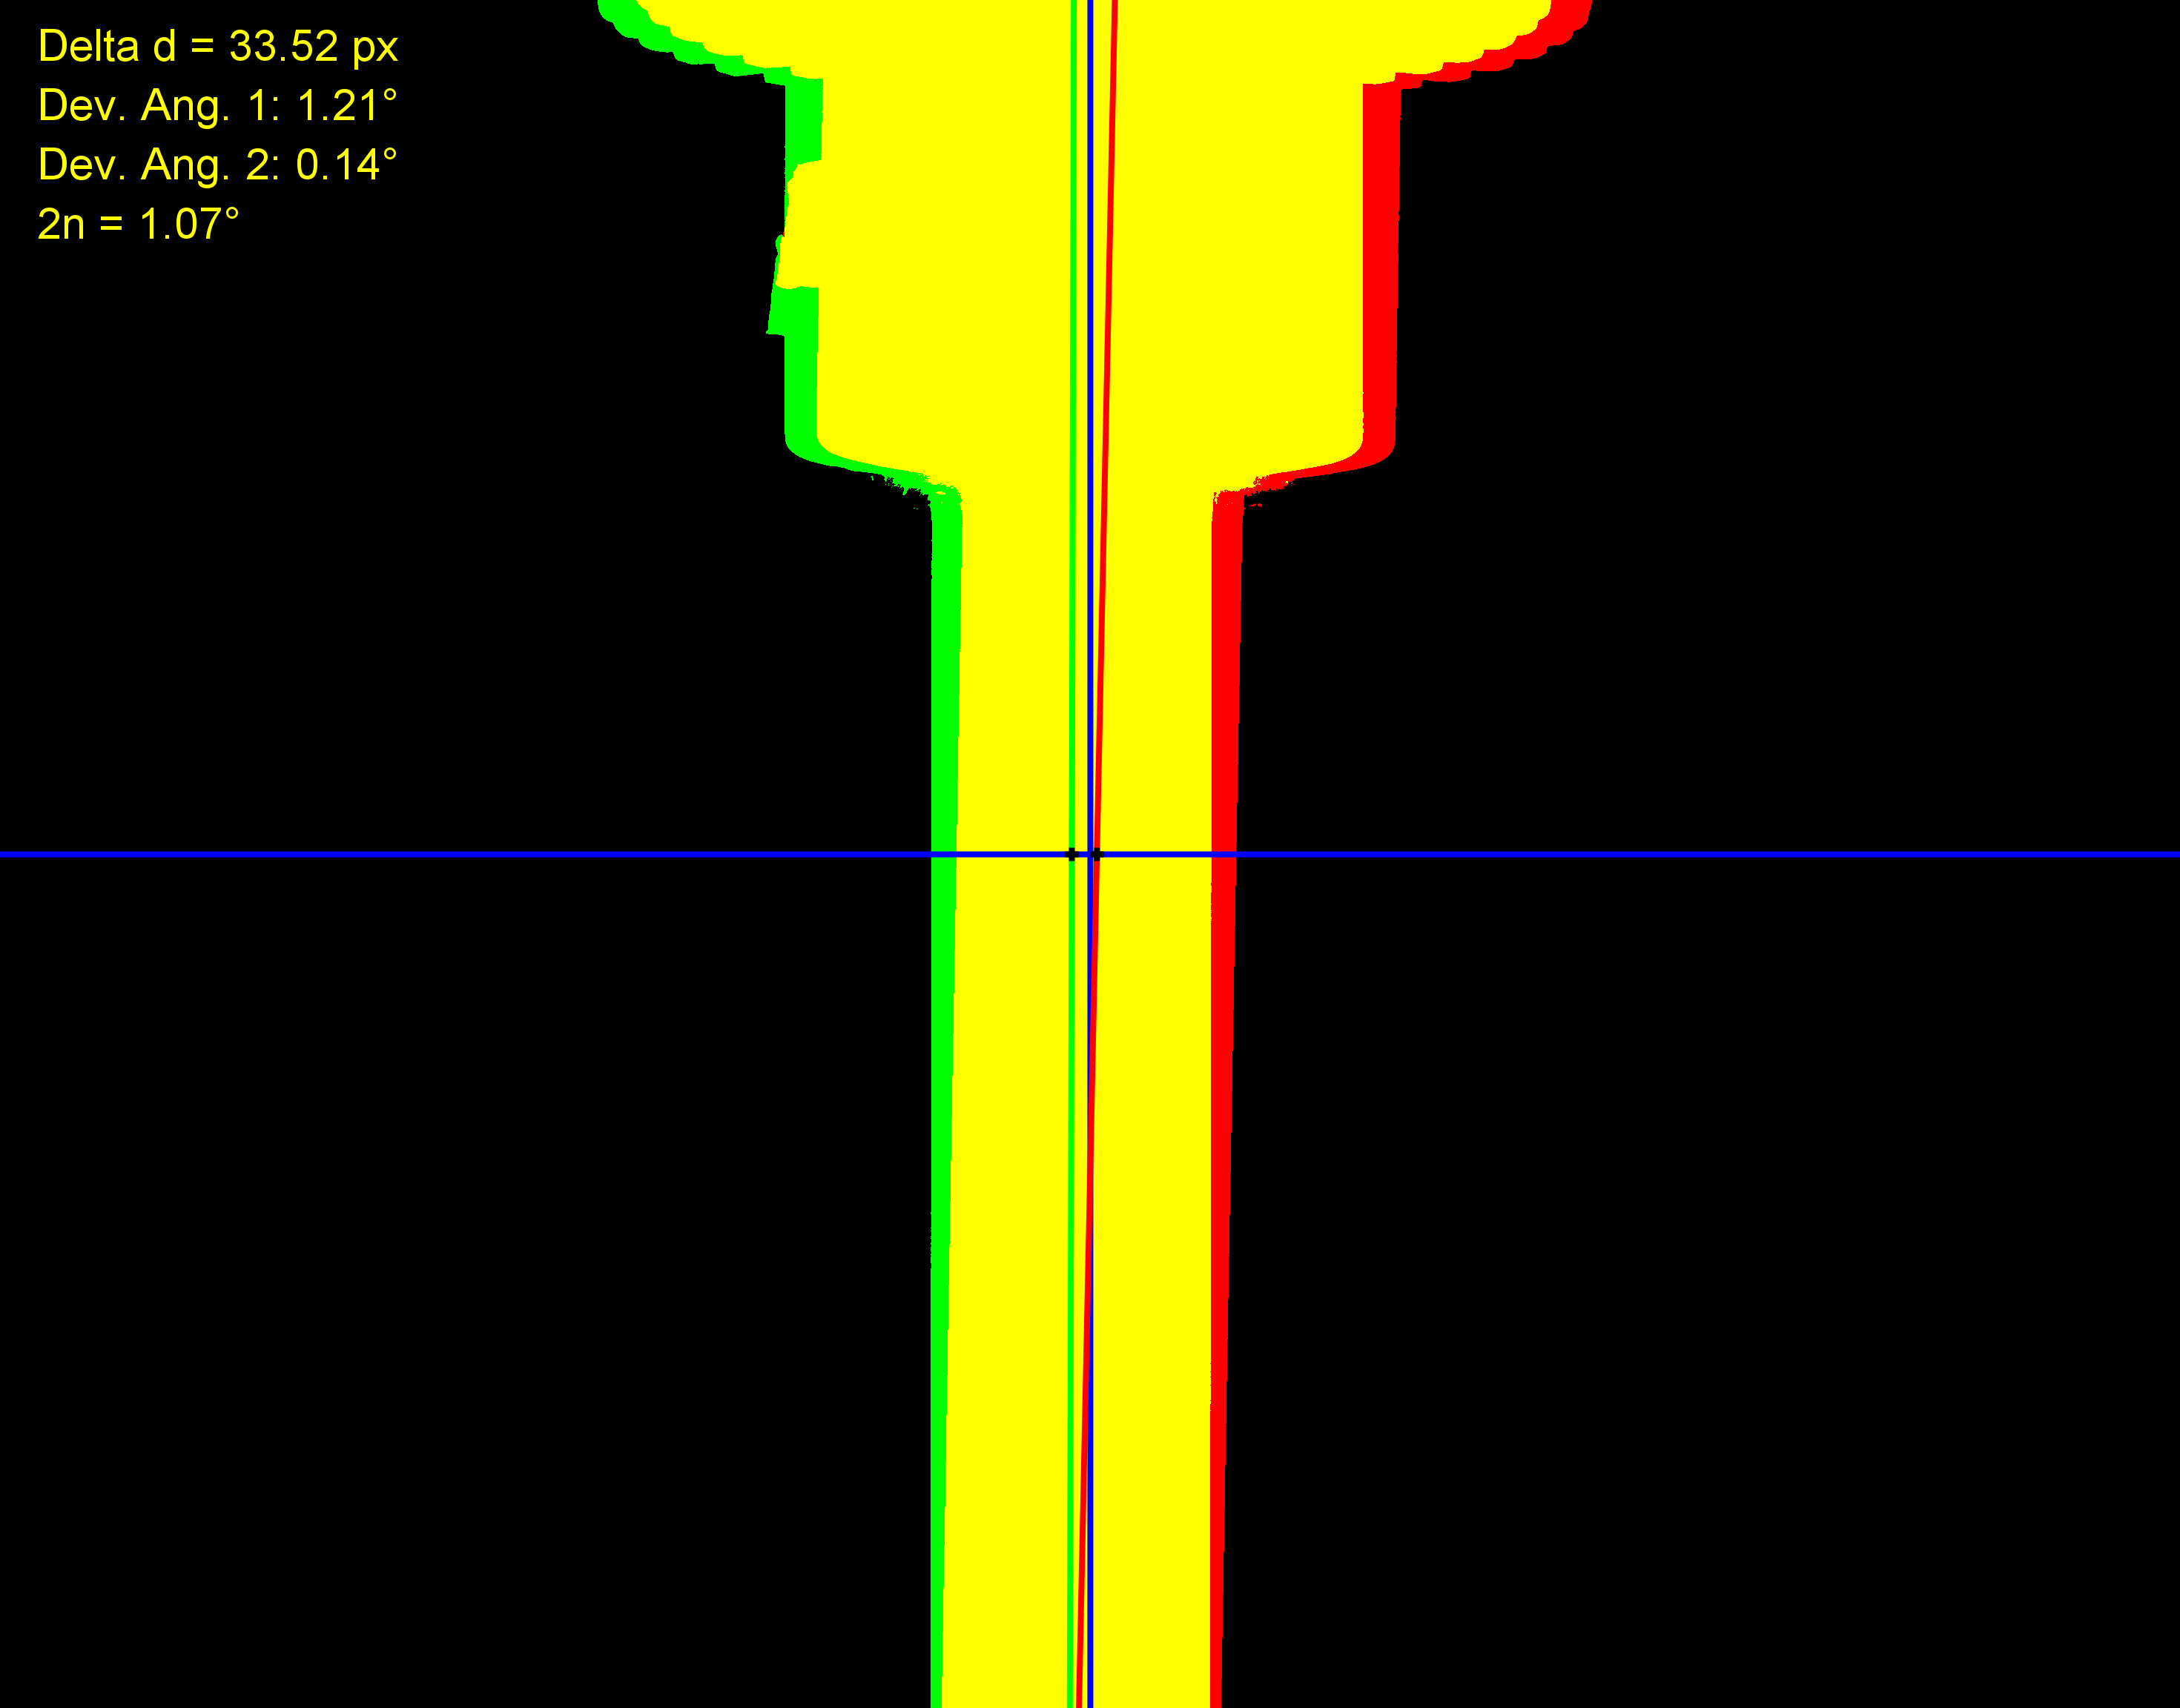
\includegraphics[width=\textwidth]{images/Interseccion_cerca.png}
    \end{subfigure}
    \hfill
    \begin{subfigure}{0.49\textwidth}
        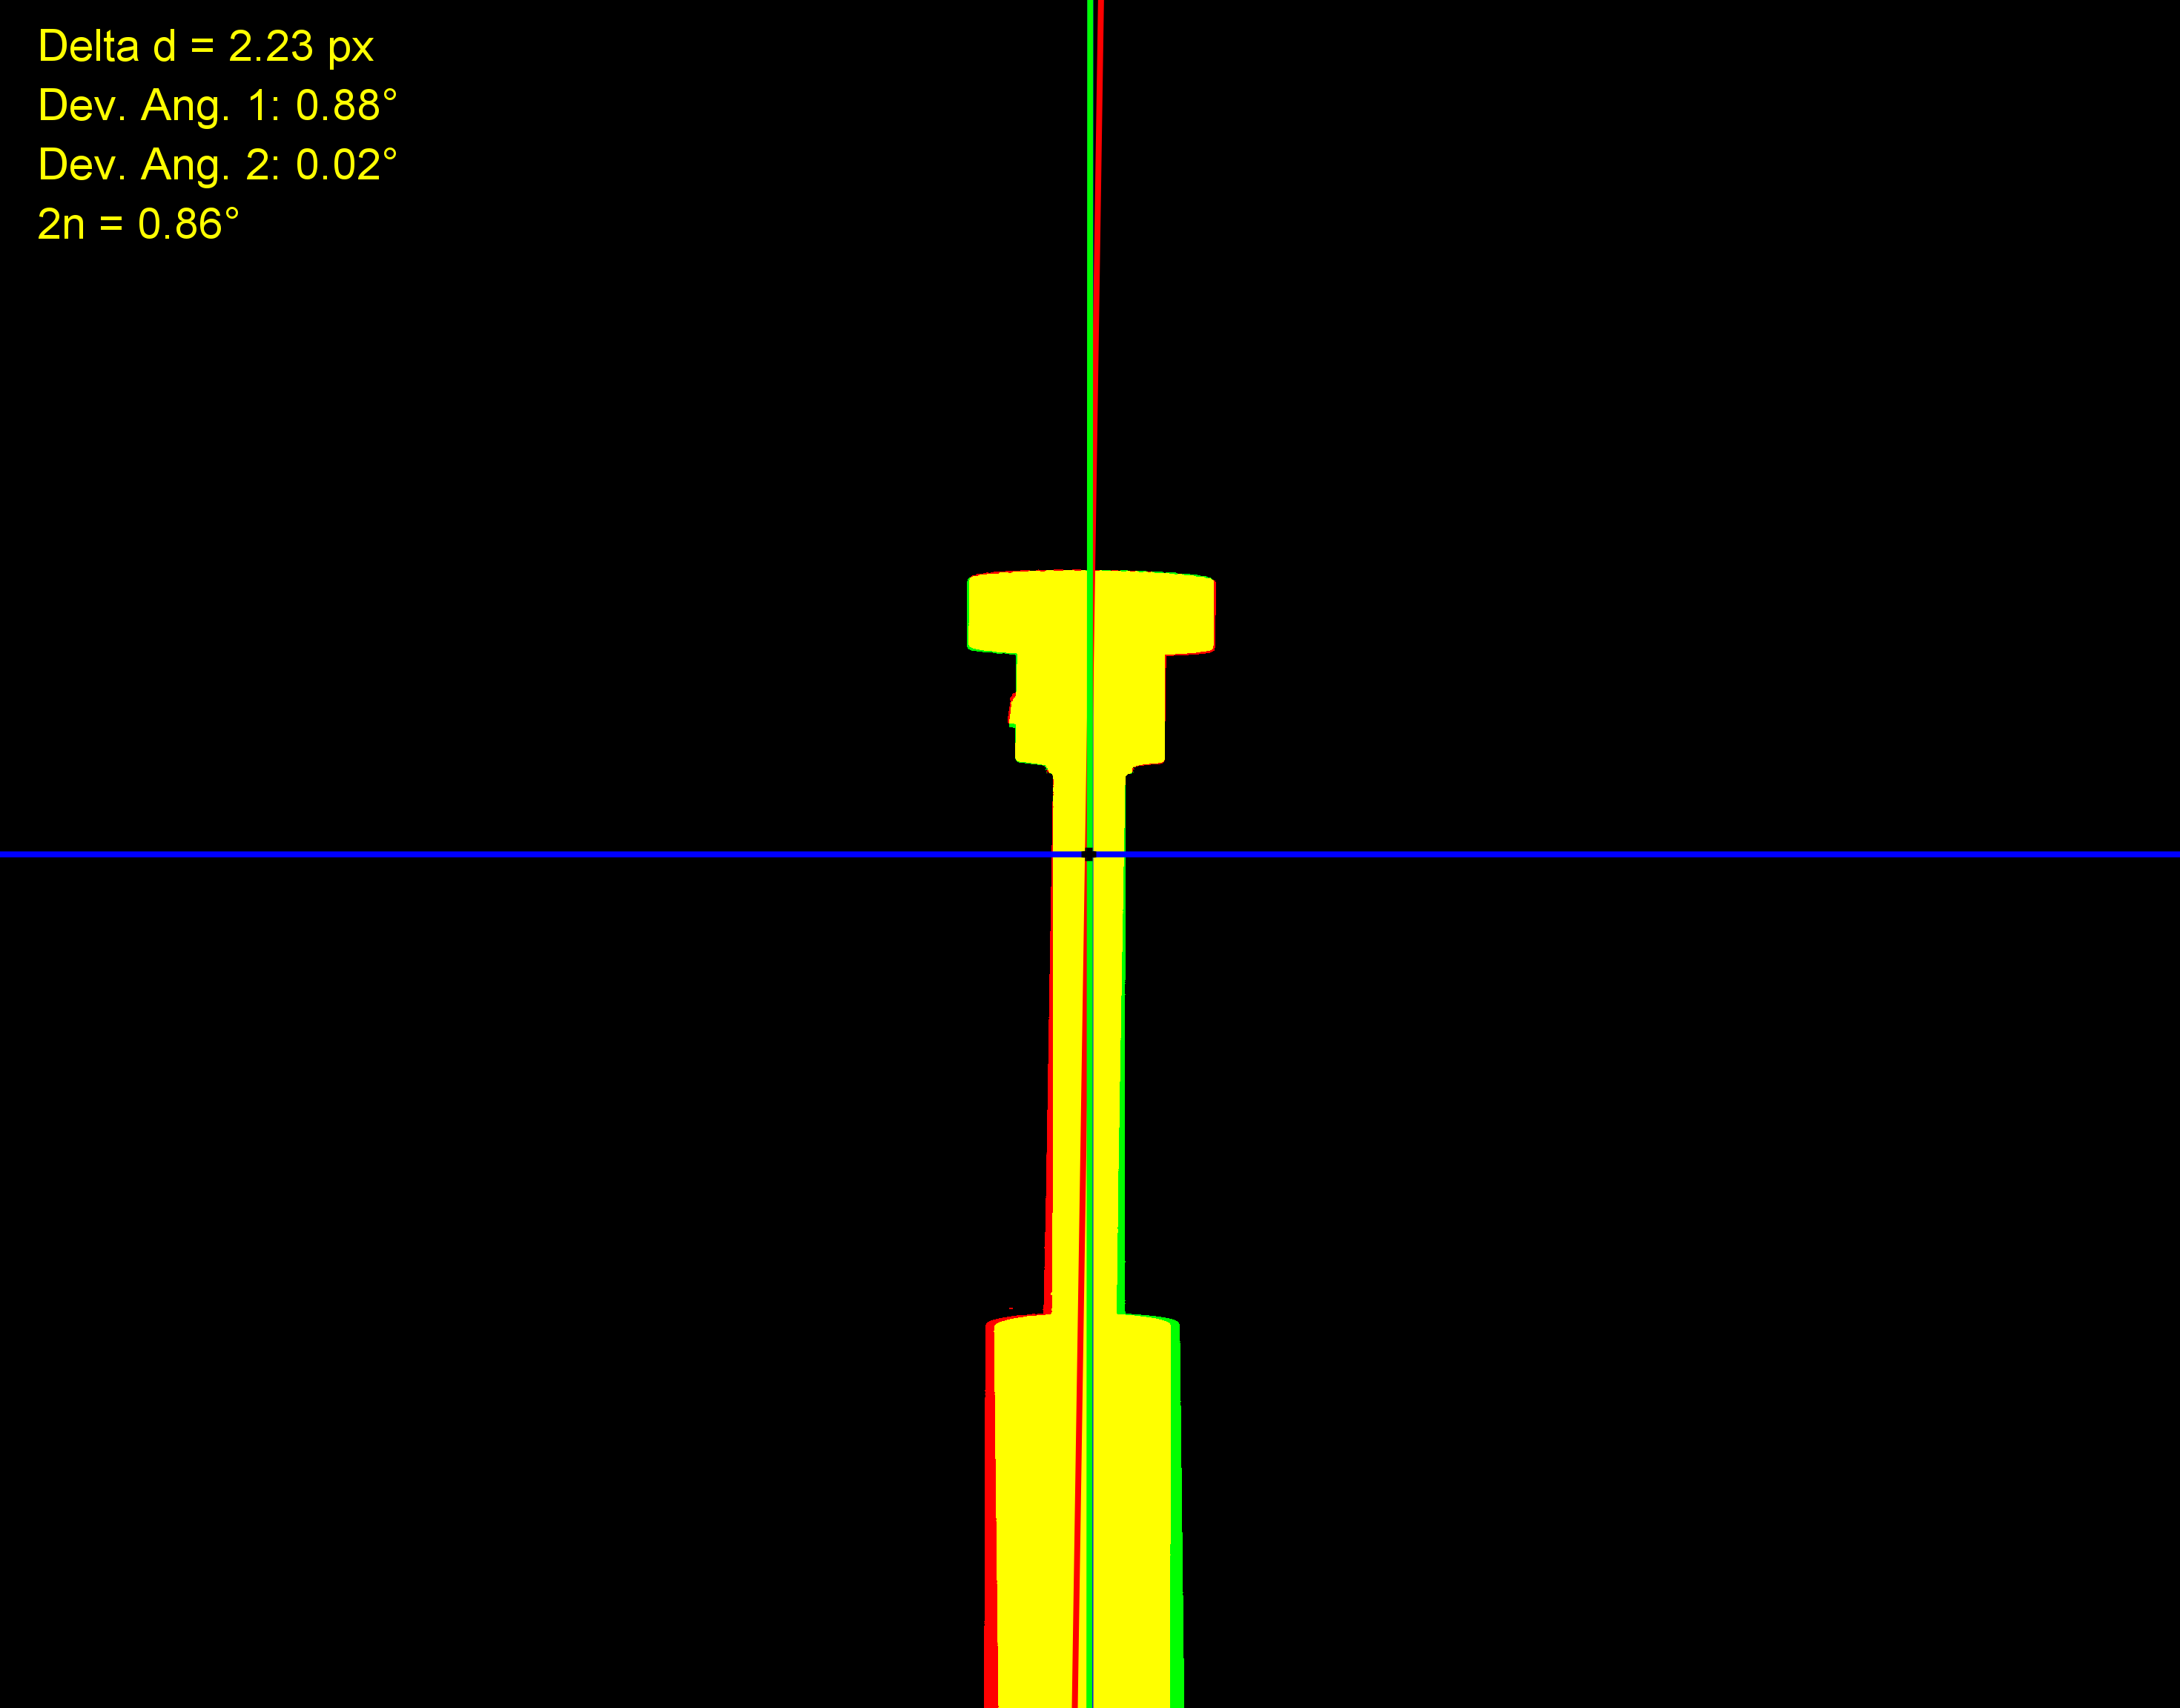
\includegraphics[width=\textwidth]{images/Interseccion_lejos.png}
    \end{subfigure}
    \caption{Cada imagen es la superposición de dos proyecciones del mismo objeto en una posición
    $\hat{x}$ (\textit{izq.} cercana a la fuente y \textit{der.} lejana). La región color verde es
    el reflejo horizontal de la proyección del objeto rotado 180$^{\circ}$ respecto de la posición original
    (rojo), y la amarilla es la superposición de ambos. Se determinan los ejes de rotación de cada
    objeto, el ángulo $2\eta$ entre ambos, y los puntos de intersección de los ejes de rotación con
    $U=0$, utilizados para determinar la distancia $\Delta d$ entre ejes.}
    \label{fig:res_alin_muestra}
\end{figure}

Los resultados anteriores son estimaciones que se obtuvieron al intentar reducir las desalineaciones
al mínimo posible, manipulando el hardware directamente. Se encuentran resumidos en la tabla
\ref{tabl:alineacion}.

Una vez realizada la alineación general, se procedió a aplicar los métodos de múltiples proyecciones
y de única proyección para
determinar las correcciones necesarias, como se explicó anteriormente. En la figura
\ref{fig:res_yang}.a se puede observar una proyección arbitraria del fantoma superpuesta
sobre un gráfico con todas las posiciones de cada una
de las esferas, a lo largo de la rotación. Por otro lado, la figura \ref{fig:res_yang}.b
muestra las elipses ajustadas a partir de las posiciones medidas, correspondientes a cada esfera,
y los puntos de interés $\vec{p}_{ij}$ ($j=0,1,2,3,4$). A partir de dichos puntos, se
realizaron los ajustes lineales necesarios (fig. \ref{fig:res_yang}.c y \ref{fig:res_yang}.d), para determinar
los valores de $\Delta U$, $\Delta V$, $\eta$ y $D$. Por último, se determinó el valor de $F$ a partir de la ecuación \ref{eq:F}, con
$l=(28.0 \pm 0.1)$ mm, la distancia entre los centros de la primera y última esfera. 

Todo el procedimiento antes explicado se realizó también al modificar el microtomógrafo y volver
a alinearlo, con las mismas distancias cercana y lejana ($D_1$ y $D_2$), y con una distancia
final (medida con instrumento) de $D = (256 \pm 1)$ mm. No se utilizó el método de una única
proyección en este caso, ya que su inconsistencia e imprecisión ya se había demostrado (ver siguiente
sección).

En la tabla \ref{tabl:alineacion}
se exponen todos los resultados de distintas mediciones con ambos métodos (junto con los valores
de $D_m$ y $F_m$ medidos con instrumentos). En particular, las mediciones marcadas con color gris
fueron realizadas tras una realineación del eje de movimiento del porta-muestra, mientras que las
color amarillo corresponden a la última modificación del microtomógrafo (con el detector en ``vertical'').
Las incertidumbres se determinaron a partir de
los ajustes finales, en el caso de los parámetros $\Delta U$, $\Delta V$, $\eta$ y $D$. Para $F$,
se tomó como incertidumbre la propagación de errores en la ecuación \ref{eq:F}, utilizando la incertidumbre
obtenida para $D$ y la estimada para $l$. Para las distancias entre puntos $\vec{p}_{ij}$, se tuvo en cuenta
que las elipses elegidas para el cálculo (la primera y la última) son las que mejor ajustan los datos,
y se observó un error geométrico menor a 0.5 px. Por otro lado,
en la tabla \ref{tabl:ajustes} se observan los valores del coeficiente de determinación $R^2$ de
todos los ajustes por regresión lineal realizados durante una medición (ocho elipses y dos rectas),
específicamente, de la cuarta medición de la tabla \ref{tabl:alineacion}, que es representativa
de todas las mediciones.


\begin{table}[htbp]
    \centering
    \caption{Parámetros de alineación y correcciones geométricas.}
    % Ajustes de reducción
    \small 
    \setlength{\tabcolsep}{4pt} % El valor por defecto es 6pt
    \begin{tabular}{ccccccc} % 7 columnas centradas
        \toprule
        \rowcolor{gray!30} \multicolumn{7}{c}{\textbf{Alineación general}} \\ \midrule
        $D$ (mm) & $\Delta \hat{Y}$ (mm) & $\theta$ ($^{\circ}$) & $\phi$ ($^{\circ}$) & $\Delta U$ (px) & $\Delta V$ (px) & $\eta$ ($^{\circ}$) \\ \midrule
        $258 \pm 1$ & $<2$ & $<4$ & $<4$ & $<5$ & $<5$ & $0.48 \pm 0.06$  \\
        \rowcolor{yellow!30} $256 \pm 1$ & $<2$ & $<4$ & $<4$ & $<9$ & $<4$ & $-0.37 \pm 0.02$  \\
        \\ \midrule % Espacio para datos

        \rowcolor{gray!30} \multicolumn{7}{c}{\textbf{Correcciones por método de múltiples proyecciones}} \\ \midrule
        $D_m$ (mm) & $F_m$ (mm) & $D$ (mm) & $F$ (mm) & $\Delta U$ (px) & $\Delta V$ (px) & $\eta$ ($^{\circ}$) \\ \midrule
        $258 \pm 1$ & $71 \pm 1$ & $268.7 \pm 0.8$ & $80.1 \pm 0.6$ & $15.0 \pm 0.9$ & $21.6 \pm 0.6$ & $0.45 \pm 0.02$ \\
        $258 \pm 1$ & $107 \pm 1$ & $266.6 \pm 0.5$ & $106.2 \pm 0.5$ & $22.4 \pm 0.7$ & $22.4 \pm 0.5$ & $0.50 \pm 0.03$ \\
        $258 \pm 1$ & $79 \pm 1$ & $267.9 \pm 0.6$ & $77.4 \pm 0.4$ & $29.6 \pm 0.7$ & $22.4 \pm 0.5$ & $0.52 \pm 0.03$ \\ \midrule
        \rowcolor{gray!15} $258 \pm 1$ & $88 \pm 1$ & $267.5 \pm 0.5$ & $87.2 \pm 0.3$ & $1.4 \pm 0.1$ & $21.6 \pm 0.5$ & $0.46 \pm 0.01$ \\
        \rowcolor{gray!15} $258 \pm 1$ & $133 \pm 1$ & $266.3 \pm 0.5$ & $132.2 \pm 0.4$ & $1.6 \pm 0.1$ & $22.6 \pm 0.5$ & $0.49 \pm 0.01$ \\ \midrule
        \rowcolor{yellow!30} $256 \pm 1$ & $93 \pm 1$ & $264.6 \pm 0.3$ & $93.1 \pm 0.4$ & $3 \pm 1$ & $-14 \pm 1$ & $-0.33 \pm 0.02$ \\
        \\ \midrule
        
        \rowcolor{gray!30} \multicolumn{7}{c}{\textbf{Correcciones por método de una proyección}} \\ \midrule
        $D_m$ (mm) & $F_m$ (mm) & $D$ (mm) & $F$ (mm) & $\Delta U$ (px) & $\Delta V$ (px) & $\eta$ ($^{\circ}$) \\ \midrule
        \rowcolor{gray!15}$258 \pm 1$ & $175 \pm 1$ & $211 \pm 2$ & $136 \pm 1$ & $-3.6 \pm 0.5$ & $11 \pm 1$ & $-39 \pm 1$ \\
        \rowcolor{gray!15}$258 \pm 1$ & $114 \pm 1$ & $264.1 \pm 0.9$ & $117 \pm 1$ & $0.5 \pm 0.9$ & $1.1 \pm 0.5$ & $2.3 \pm 0.7$ \\
        \rowcolor{gray!15}$258 \pm 1$ & $220 \pm 1$ & $264 \pm 1$ & $225 \pm 1$ & $-2 \pm 1$ & $-5 \pm 1$ & $-17 \pm 2$ \\
        \rowcolor{gray!15}$258 \pm 1$ & $220 \pm 1$ & $265 \pm 1$ & $226 \pm 1$ & $-13 \pm 2$ & $10 \pm 2$ & $48 \pm 4$ \\
        \bottomrule
    \end{tabular}
\label{tabl:alineacion}
\end{table}

\begin{table}[htbp]
\centering
\caption{Coeficientes de determinación de ajustes, para método de Yang.}
\begin{tabular}{cccccccccc}
    \toprule
    \rowcolor{gray!30} \multicolumn{10}{c}{\textbf{Coeficiente de determinación $R^2$}} \\ \midrule
    Esf 1 & Esf 2 & Esf 3 & Esf 4 & Esf 5 & Esf 6 & Esf 7 & Esf 8 & $\{ D, \Delta V \}$ & $\{\eta, \Delta U \}$ \\ \midrule
    \rowcolor{gray!15} $0.997$ & $0.995$ & $0.985$ & $0.891$ & $0.857$ & $0.996$ & $0.999$ & $0.999$ & $0.999$ & $0.998$ \\
    \rowcolor{yellow!30} $0.998$ & $0.996$ & $0.988$ & $0.864$ & $0.958$ & $0.998$ & $0.999$ & $0.999$ & $0.999$ & $0.980$ \\ \bottomrule
\end{tabular}
\label{tabl:ajustes}
\end{table}

\begin{figure}[htbp] % Se recomienda htbp en lugar de h para dar más opciones de posicionamiento al compilador
    \centering
    % Primera fila
    \begin{overpic}[width=0.49\linewidth]{images/plot_centroids2.png}
        \put(2, 75){\colorbox{black!50}{\color{white}\bfseries\large (a)}}
    \end{overpic}\hfill
    \begin{overpic}[width=0.49\linewidth]{images/fit_elipses.png}
        \put(2, 75){\colorbox{black!50}{\color{white}\bfseries\large (b)}}
    \end{overpic}
    
    \vspace{2ex} % Espaciado entre filas
    
    % Segunda fila
    \begin{overpic}[width=0.49\linewidth]{images/yang_fit_1.png}
        \put(2, 75){\colorbox{black!50}{\color{white}\bfseries\large (c)}}
    \end{overpic}\hfill
    \begin{overpic}[width=0.49\linewidth]{images/yang_fit_2.png}
        \put(2, 75){\colorbox{black!50}{\color{white}\bfseries\large (d)}}
    \end{overpic}
    
    \caption{\textbf{a)} Una proyección arbitraria del fantoma, puesta sobre un gráfico que
    contiene las posiciones de todos los centros de las esferas, a lo largo de toda su trayectoria
    en 360$^{\circ}$. \textbf{b)} Elipses ajustadas a partir de las posiciones medidas, con los puntos de interés $\vec{p}_{ij}$ marcados (centros y vértices).
    \textbf{c)} Ajuste lineal de los puntos $(x_i,y_i)$ definidos en la ecuación
    \ref{eq:variables_yang1}. A partir de los parámetros $\mathsf{a}_1$ y $\mathsf{b}_1$
    se pueden obtener los valores de $D$ y $\Delta V$. \textbf{d)} Ajuste lineal de los
    puntos $(v_{i0},u_{i0})$; a partir de los parámetros $\mathsf{a}_2$ y $\mathsf{b}_2$
    se pueden calcular $\Delta U$ y $\eta$.}
    \label{fig:res_yang}
\end{figure}

\section{Resolución espacial}

\subsection{Análisis por MTF}

Uno de los objetivos de la calibración geométrica, es poder determinar con precisión
la resolución espacial de una tomografía/radiografía, ya que de esta dependen todas las
mediciones de distancias que se quieran realizar. La ecuación \ref{eq:res_espacial},
aunque más completa que solo considerar la magnificación de un objeto por una fuente
puntual, sigue siendo una aproximación, ya que la resolución depende de todos los elementos
del sistema (fuente, objeto, detector, electrónica, algoritmos, etc.). Sin embargo,
esta se puede medir directamente en una radiografía.

El método más directo consiste en utilizar un objeto de referencia, con detalles de
tamaño similar a la resolución (por ejemplo, líneas y círculos). El problema es que,
para microtomógrafos con resolución en el orden de micrómetros, es difícil producir
fantomas apropiados. El método más común es el análisis de bordes por medio de la
función de transferencia de modulación (\textit{Modulation Transfer Function} - $MTF$)\cite{Buzug2008}.
La $MTF$ es una función que relaciona la frecuencia espacial a la correspondiente
pérdida de contraste en la imagen, y se define como la transformada de Fourier de la
derivada de la función de dispersión de borde (\textit{Edge Spread Function} - $ESF$), y se define normalizada. La $ESF$ es la función de
contraste o intensidad $I(x)$, en la dirección $x$ que atraviesa perpendicularmente una interfaz o borde,
y su derivada se conoce como la función de transferencia de línea (\textit{Line Transfer
Function} - $LSF$). \cite{Samei1998}\cite{Rueckel2014}

\begin{equation}
    MTF(k_x) = \dfrac{\mathcal{F}\left\{LSF(x)\right\}}{MTF(0)} =
    \dfrac{\mathcal{F}\left\{\dfrac{d}{dx}ESF(x)\right\}}{MTF(0)}
    \label{eq:MTF}
\end{equation}

\noindent donde $\mathcal{F}\left\{f(x)\right\}(k_x)$ es la Transformada de Fourier de la
función $f(x)$, del dominio espacial $x$ al dominio de frecuencias $k_x$.

A medida que aumenta la frecuencia espacial $k_x$ en la dirección $x$, mayor es la pérdida
de constraste, es decir, mientras más cercanos sean dos detalles distintos (líneas o puntos),
más difícil es diferenciarlos en la imagen. Para obtener un valor específico de la
resolución espacial, en general se considera la frecuencia espacial $k_c$ a la que la
función $MTF$ cae al 10$\%$ \cite{Ruf2020}, de la que puede obtenerse el valor correspondiente en el
dominio espacial mediante la ecuación \ref{eq:res_espacial}.

A partir de esto, se midió la $MTF$ de dos formas. En la primera, se utilizó como fantoma
una lámina metálica, de ancho $w_{lamina}= (12.56\pm 0.02)$ mm y borde recto, fijada por un marco de acrílico de
tal forma que hay una sección de solo aire y metal (ver figura \ref{fig:chapita}.a). El fantoma se coloca en el porta-muestra,
idealmente perpendicular al eje del haz, y se obtienen proyecciones a distintas
magnificaciones $M$. El borde de la lámina debe estar inclinado con respecto a los ejes
$(u,v)$, para evitar posibles distorsiones por filas/columnas de pixeles en el detector.
El borde es rotado en el procesamiento de la imagen, para alinearlo nuevamente, y se mide
el perfil de contraste entre el aire y la lámina (en una dirección perpendicular al borde).
En concreto, se mide el valor medio de cada columna $x$, $VM|_{y_0}^{y_f}(x)$, en un ROI alrededor del borde.
Posteriormente, se interpola la función $ESF(x)$ a partir de los puntos obtenidos,
y se calcula la derivada numérica. Finalmente, se realiza una transformada de Fourier rápida (FFT) y,
normalizando con el valor correspondiente a $k_x = 0$, se obtiene la $MTF(k_x)$. Para obtener
un valor más representativo de todo el borde, se realizan múltiples mediciones en distintos
ROIs a lo largo del borde (utilizando un \textit{macro} en FIJI, ver Apéndice B.4), como se observa en la figura
\ref{fig:chapita}.b.

\begin{figure}[htpb]
    \centering
    \begin{subfigure}{0.35\textwidth}
        \begin{overpic}[width=\linewidth]{images/phantom_chapita.jpg}
            \put(2, 87){\colorbox{black!60}{\color{white}\bfseries\large (a)}}
        \end{overpic}
    \end{subfigure}
    \hspace{5mm}
    \begin{subfigure}{0.45\textwidth}
        \begin{overpic}[width=\linewidth]{images/chapita_esf.png}
            \put(2, 68){\colorbox{black!60}{\color{white}\bfseries\large (b)}}
        \end{overpic}
    \end{subfigure}
    \caption{\textbf{a)} Fantoma utilizado para medir resolución espacial de una
    proyección. Lámina delgada de metal, en contacto con aire y ligeramente inclinada
    con respecto a los ejes del detector. \textbf{b)} Proyección del fantoma. Los
    rectángulos rojos son los ROIs sobre los que se analiza el perfil de intensidad, en
    la dirección del lado largo.}
    \label{fig:chapita}    
\end{figure}

Para la interpolación de $ESF(x)$, se realiza un ajuste polinómico móvil de orden 4 con peso gaussiano,
es decir, se ajusta un polinomio de orden 4 a los datos dentro de una ``ventana'' de
ancho $w_v$, la cual se va desplazando por todo el set. A partir de los coeficientes
obtenidos en cada ventana, es posible interpolar los puntos cercanos a cada dato. 
Para un polinomio de orden 4, $w_v$ debe contener al menos cuatro puntos consecutivos
(cinco si se cuenta el punto central), y mientras más grande es, produce un mayor
suavizado de la función (lo cual puede afectar el resultado del $MTF$) \cite{Samei1998}.
Para este trabajo, se utilizó $w_v = 5$ y una interpolación de factor 2 (se duplica
la cantidad de datos). Por otro lado, para obtener una medición más ``limpia'' del $MTF$
se recomienda aplicar un filtro de Hamming a la $LSF$, con tal de eliminar los componentes
de frecuencias altas.

Sin embargo, este método determina la resolución espacial de una radiografía, y aunque
la intuición indica que esta debería ser la misma que una tomografía, esta podría ser
alterada por algún efecto de la reconstrucción. Luego, se realizó el siguiente método para
medir la resolución espacial de una tomografía, basado en la investigación de Ruf \textit{et al.}
\cite{Ruf2020}. La idea es obtener una reconstrucción de un fantoma cilíndrico, y aplicar
el mismo procedimiento que con la lámina, pero analizando distintas slices (cortes 
transversales) o cortes sagitales a lo largo del diámetro completo (ver fig. 
\ref{fig:fantoma_MTF}). Así, se pueden obtener mediciones de la resolución espacial de 
la tomografía, en distintas direcciones de reconstrucción. Para obtener dichos cortes,
se utilizó un \textit{macro} (ver Apéndice B.5).

\begin{figure}[htbp]
    \centering
    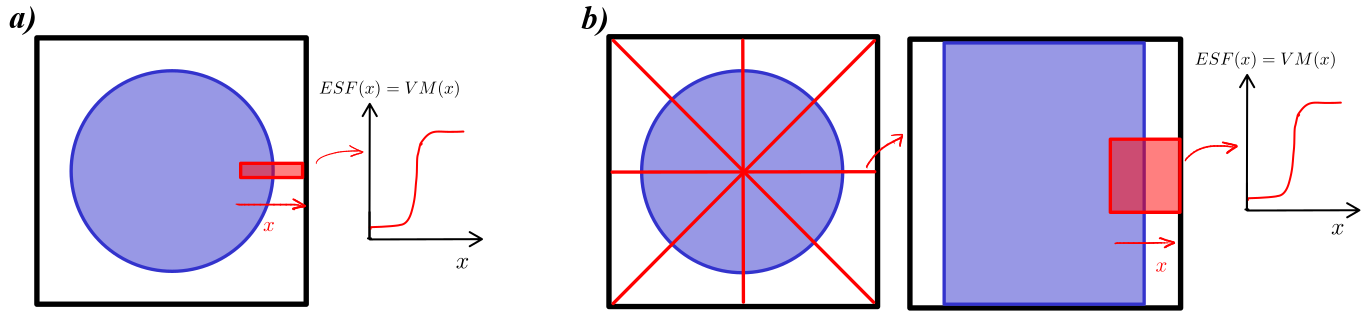
\includegraphics[width=\textwidth]{images/fantoma_MTF.png}
    \caption{Proceso de medición del $ESF(x)$ en una reconstrucción tomográfica de un
    cilindro. \textbf{a)} Adquisición de $ESF(x)$ en un corte axial, seleccionando una
    región alrededor del borde, con la menor curvatura posible. \textbf{b)} Adquisición
    de $ESF(x)$ en un plano sagital, seleccionando una región alrededor del borde.}
    \label{fig:fantoma_MTF}
\end{figure}

\subsection{Resultados}

En la figura \ref{fig:res_mtf_1} pueden observarse tres gráficos (a, b y c) representativos de
todo el proceso (utilizando la lámina): la adquisición e interpolación de la $ESF(x)$, la derivada o $LSF(x)$
y la obtención de la $MTF(k_x)$, para una magnificación específica. La figura \ref{fig:res_mtf_1}.d
muestra las mediciones obtenidas de la resolución espacial a partir de este método, para
distintas magnificaciones, en cada uno de los sistemas alineados (rojo, sistema inicial con
detector horizontal; azul, sistema final con detector vertical), y las compara con las curvas correspondientes a la ecuación
\ref{eq:res_espacial} (para tamaños focales $s_1 = 0.005$ mm y $s_2 = 0.007$ mm, correspondientes a
la fuente utilizada). Los valores de resolución
espacial se calcularon como $RE = 1/(2k_c)$, donde $k_c$ es la frecuencia de corte ($MTF(k_c)=0.1$).
La incertidumbre se calculó propagando la incertidumbre de $k_c$, la cual fue definida como
el error estadístico a partir de 10 mediciones de $MTF$ a lo largo del borde.

También, a partir de las mediciones de resolución espacial en conjunto, se realizó un ajuste de los
datos a la siguiente curva, basada en la ecuación \ref{eq:res_espacial}, pero agregando un parámetro
extra $c$ que contribuye al tamaño de pixel $\Delta p$, y con $S=s_2$. El mismo se encuentra
graficado en la figura \ref{fig:res_mtf_1}.d, y tiene un coeficiente de determinación $R^2 = 0.983$ y
un valor del parámetro ajustado $c=(0.0264 \pm 0.0008)$ mm.

\begin{equation}
    RE(M) = \sqrt{\left(S\cdot\dfrac{M-1}{M}\right)^2 + \left(\dfrac{\Delta p+c}{M}\right)^2}
    \label{eq:ajuste_resolucion}
\end{equation}

Por otro lado, para el análisis de la resolución espacial de una tomografía, se utilizó una
reconstrucción de un cilindro con una magnificación $M\sim 5.2$. Se analizó el perfil
de intensidad de borde en 10 re-proyecciones radiales. Los gráficos de $ESF(x)$, $LSF(x)$
y $MTF(x)$ pueden observarse en la figura \ref{fig:res_mtf_2}. Promediando los valores
de frecuencia de corte se obtiene que, para esta magnificación, $k_c = (28.5 \pm 0.3)$ lp/mm,
y la resolución espacial, $RE = (17.5 \pm 0.2)$ $\mu$m, valor que se agregó al gráfico de la
figura \ref{fig:res_mtf_1}.d.

\begin{figure}[htbp]
    \centering
    % Primera fila
    \begin{overpic}[width=0.49\linewidth]{images/ESF.png}
        \put(2, 75){\colorbox{black!50}{\color{white}\bfseries\large (a)}}
    \end{overpic}\hfill
    \begin{overpic}[width=0.49\linewidth]{images/LSF.png}
        \put(2, 75){\colorbox{black!50}{\color{white}\bfseries\large (b)}}
    \end{overpic}
    
    \vspace{2ex} % Espaciado entre filas
    
    % Segunda fila
    \begin{overpic}[width=0.49\linewidth]{images/MTF_1.png}
        \put(2, 75){\colorbox{black!50}{\color{white}\bfseries\large (c)}}
    \end{overpic}\hfill
    \begin{overpic}[width=0.49\linewidth]{images/resolucion.png}
        \put(2, 75){\colorbox{black!50}{\color{white}\bfseries\large (d)}}
    \end{overpic}
    
    \caption{\textbf{a)} Función $ESF(x)$ ajustada al perfil de intensidad de un
    ROI alrededor de un borde. \textbf{b)} Función $LSF(x)$, derivada numérica de $ESF(x)$.
    \textbf{c)} Función $MTF(k_x)$, la transformada de Fourier de $LSF(x)$ y normalizada. El
    valor de $k_x$ para el que $MTF=0.1$ se denomina \textit{frecuencia de corte} $k_c$,
    y es considerada como la resolución espacial del sistema. \textbf{d)} Mediciones de
    $RE$ en función de la magnificación $M$, a partir de un promedio de 10 mediciones de
    $MTF$ cada una, de las dos configuraciones del sistema (rojo para el detector horizontal;
    azul para el detector vertical); también se grafican las curvas de resolución mínima ideal (para tamaños
    de foco $s_1$ y $s_2$), y la curva de ajuste a los datos en conjunto (ecuación \ref{eq:ajuste_resolucion}),
    y la medición de $RE$ obtenida a partir de una reconstrucción tomográfica.}
    \label{fig:res_mtf_1}
\end{figure}

\begin{figure}[htbp]
    \centering
    \begin{subfigure}{0.32\textwidth}
        \begin{overpic}[width=\linewidth]{images/ESF_tomgr.png}
            \put(2, 75){\colorbox{black!50}{\color{white}\bfseries\large (a)}}
        \end{overpic}        
    \end{subfigure}
    \hfill
    \begin{subfigure}{0.32\textwidth}
        \begin{overpic}[width=\linewidth]{images/LSF_tomgr.png}
            \put(2, 75){\colorbox{black!50}{\color{white}\bfseries\large (b)}}
        \end{overpic}        
    \end{subfigure}
    \hfill
    \begin{subfigure}{0.32\textwidth}
        \begin{overpic}[width=\linewidth]{images/MTF_2.png}
            \put(2, 75){\colorbox{black!50}{\color{white}\bfseries\large (c)}}
        \end{overpic}        
    \end{subfigure}
    \caption{\textbf{a)} $ESF(x)$ de distintos cortes radiales de la reconstrucción tomográfica
    de un cilindro metálico. \textbf{b)} $LSF(x)$ de los distintos cortes. \textbf{c)}
    $MTF(k_x)$ de los distintos cortes reconstruidos, y $MTF_{promedio}$.}
    \label{fig:res_mtf_2}
\end{figure}

\section{Discusiones}

\subsection{Alineación y correcciones}

Observando los resultados de la tabla \ref{tabl:alineacion}, se puede ver que una buena alineación
general es posible de lograr, utilizando los métodos de análisis de círculos proyectados y
superposición de cilindros rotados. La figura \ref{fig:alineacion_fuente} muestra que los círculos
proyectados alcanzan criterios de circularidad satisfactorios, con $C_W \sim 90\%$ y $R \sim 99\%$.
La razón por la que $C_W$ no es mayor, se debe a que el cálculo de perímetro y área se realiza
contando píxeles en una grilla discreta, lo que produce un error geométrico al tratarse de una
figura curva. La importancia de estos resultados radica en la capacidad de alinear la orientación
del detector, con respecto a la fuente, llegando a lograr una desviación angular menor a 5$^{\circ}$ respecto
de la posición ideal, solamente observando una proyección.

Sin embargo, este proceso depende mucho de la destreza
del operador, por lo que es difícil de estandarizar. Otro problema relacionado con esto, es que
se asume que al mover el detector a su posición final, se hace a lo largo de un eje que une
las posiciones cercana y lejana. Sin embargo, este traslado está lejos de ser ideal, debido al
juego mecánico de la base sobre la que se mueve, los tornillos de ajuste, la fricción, etc. Este
problema puede solucionarse mejorando el sistema de la base, utilizando mejores piezas y rieles,
y en última instancia, con un sistema de movimiento motorizado, que asegure un traslado suave
y consistente. Por esta razón es que se observan diferencias entre los parámetros $\Delta U$ y $\Delta V$ obtenidos
con los métodos de proyecciones, con respecto a los valores esperados a partir de la alineación general.

Una utilidad de este método, es la posibilidad de estimar los ángulos $\theta$ y $\phi$, o más bien,
demostrar que estos son lo suficientemente pequeños como para aplicar el método de múltiples proyecciones
posteriormente. Esto se mantiene en la posición final, utilizando escuadras y niveles. Sin
embargo, no es posible medirlos con mayor precisión, debido a no poder estudiar el círculo
proyecado.

Sobre el análisis de la superposición de cilindros rotados, se observa en la tabla que los resultados
estimados de $\eta$ son comparables a los obtenidos con el método de múltiples proyecciones, por lo que es
viable como un método más rápido para determinar este parámetro. Sin embargo, se presenta otro
problema, difícil de contemplar en el análisis: el método asume que el cilindro está perfectamente
alineado con el eje de rotación del porta-muestra (esta asunción se hace con cualquier muestra en realidad),
sin embargo, después de estudiar numerosas veces este proceso, se observa que esto varía según el
tamaño y forma del objeto, y la forma en que se lo fija al porta-muestra. Así, se tiene que el
valor obtenido de $\eta$, a pesar de ser la inclinación del eje de rotación y ser consistente, no
necesariamente es el ángulo de inclinación del objeto, sino una aproximación a primer orden de este.
Este problema es difícil de solucionar por corrección de software, ya que dicha inclinación
varía según el objeto y no siempre es posible medirla con precisión. La solución más viable es
mejorar los sistemas de fijación de la muestra y/o bases utilizadas en el porta-muestra.
Este problema se presenta sobre todo, en muestras de gran tamaño o forma muy irregular, aunque en
muestras pequeñas no es tan prevalente.

A la hora de analizar y comparar los métodos de corrección, se tienen en cuenta tres criterios:
preparación, adquisición y resultados, siendo este último el más importante. En cuanto a la preparación
y adquisición, el método de una única proyección parece ser el más rápido y sencillo, ya que en principio
se necesita una sola radiografía del fantoma, de ahí lo atractivo del método. Y aunque es cierto
que el método de múltiples proyecciones tiene un tiempo de adquisición mucho mayor (se tardó alrededor de
20 minutos en obtener las 360 proyecciones), la preparación es relativamente sencilla comparada al otro.
En particular, el de una única proyección tiene una serie de condiciones más exigentes para su aplicación,
algunas de las cuales son prácticamente equivalentes a las condiciones de alineación general del sistema.

En primer lugar, como se mencionó en el procedimiento, el método de ``una única proyección'' requiere en realidad
más de una proyección para poder asegurar una orientación del cuadrado perpendicular con el eje
$\mathcal{M}$. Pero principalmente, este método requiere que el eje de magnificación pase justo por el centro del cuadrado. Esto
es imposible de determinar a partir de la proyección del fantoma, ya que se asume que el detector y la
fuente están desalineados (en efecto, se desea determinar $\Delta U$ y $\Delta V$), por lo que dicha
apreciación se debe realizar observando el sistema directamente. Esto es especialmente difícil cuando
el fantoma se encuentra medianamente alejado de la fuente. Quizá con mejores instrumentos de medición,
sería posible cumplir esta condición, pero a este punto la preparación del método requeriría tanto o más
esfuerzo que la alineación en sí. Además, el método es muy sensible a esta condición, como se observa en
los resultados obtenidos en la tabla \ref{tabl:alineacion}, donde las últimas dos filas de la sección de
una única proyección se corresponden a una misma distancia $F$ pero con una variación en altura del fantoma,
menor a 1.5 mm. Los resultados obtenidos para $D$ y $F$ son comparables, ya que estos dependen principalmente
de las longitudes magnificadas de los lados (que práctimante no cambian por una variación de altura tan pequeña),
pero los valores de $\Delta U$, $\Delta V$ y $\eta$ son completamente distintos. Al ser tan sensible a esta
condición, el método se vuelve inconsistente e impráctico.

Mientras tanto, el método de múltiples proyecciones requiere solamente que el cilindro esté lo suficientemente
alineado con el eje de rotación, pero no exige una altura específica, solo que el eje de magnificación
pase entre la primera y última esfera. Esto último sí puede determinarse con facilidad a partir
de la proyección, observando la excentricidad de las elipses obtenidas (mientras más excentrica una elipse
más cerca está a la altura por la que pasa el eje $\mathcal{M}$, ver figura \ref{fig:res_yang}.b).

En cuanto a los resultados, el método de múltiples proyecciones es claramente superior, ya que presenta
resultados consistentes y precisos. En la tabla \ref{tabl:alineacion} se observa que los valores obtenidos
para los distintos parámetros son comparables entre sí, a pesar de ser mediciones tomadas en distintas
distancias $F$. Solamente las primeras 3 entradas de la tabla (con fondo blanco), presentan mayor
variación en los valores de $F$, $\Delta U$ y $\eta$. Justamente a partir de la gran variación de $\Delta U$
(y no de $\Delta V$), se determinó que se debía realizar una mejor alineación del eje de movimiento
del porta-muestra. Posterior a esto, las mediciones (con fondo gris) son mucho más consistentes entre
sí en todos los parámetros, sin importar $F$. Al contrario, el método de una única proyección presenta
resultados inconsistentes entre sí, y con mucho mayor diferencia respecto a valores esperados de
la alineación general y las mediciones realizadas con instrumentos. Esto se debe, no solo a las condiciones
estrictas que se mencionaron anteriormente, sino al hecho de que los parámetros se obtienen después de
una larga cadena de operaciones matemáticas, algunas basadas en ecuaciones no lineales y sin solución
analítica, como se observa en el Apéndice A, partiendo de pocos datos (tan solo las longitudes magnificadas medidas). De esta forma, cualquier
error en la medición inicial se ve amplificado a lo largo de todo el proceso, resultando en valores tan
distintos incluso con condiciones iniciales similares.

También es importante destacar un resultado que se observa
en todas las instancias de este método, que es la diferencia entre los valores de $D_m$ (distancia
fuente-detector medida con instrumento) y $D$ obtenida a partir de los ajustes. Esta diferencia
es aproximadamente la misma en todas las mediciones (incluso al modificar el microtomógrafo), y es
un valor promedio de 9.3 mm, lo que indicaría un error sistemático en la medición de $D_m$. Esto
podría deberse a alguna característica propia del detector, de tal forma que el área donde se
produce efectivamente la detección de los fotones se encuentre alrededor de 9 mm adentro. Se
desconoce su causa ya que no se menciona nada al respecto en el manual, pero esto se corrobora
al estudiar la magnificación de un objeto de dimensiones conocidas (como el cilindro) o analizando
los círculos proyectados del cono (ver figura \ref{fig:res_alin_fuente}). En concreto, sabiendo que
el semi-ángulo de apertura del cono es 19.5$^{\circ}$, y midiendo el radio de los círculos proyectados,
se puede determinar la distancia $D$ sabiendo que $D = r/\tan(19.5\text{$^{\circ}$})$. Para los radios obtenidos
en la figura \ref{fig:res_alin_fuente}, por ejemplo, se estiman valores de $D$ mayores a los esperados
($D_1$ y $D_2$), por más de 10 mm.

Los ajustes realizados para el método de múltiples proyecciones presentan coeficientes de determinación
$R^2$ muy cercanos a 1, como se observa en la tabla \ref{tabl:ajustes}. En el caso de los ajustes de
elipses, este valor es menor para las esferas centrales, lo que se debe a una mayor excentricidad de
las mismas al estar tan cerca del eje de magnificación. Esto también se observa en la figura \ref{fig:res_yang}.d,
donde los puntos correspondientes a las esferas centrales son los que más se apartan de la recta (ya que
son determinados a partir de los ajustes de las elipses). Sin embargo, para el resto de elipses se tiene
un $R^2>0.98$, al igual que las rectas obtenidas en los ajustes posteriores, por lo que se puede concluir
que el método de múltiples proyecciones es un método confiable para determinar los parámetros de alineación
y corrección. La mayor limitación que se encontró con este método, es el hecho de que el fantoma utilizado
funciona mejor en un rango limitado de distancias, debido a la cantidad de esferas y su distribución. Sin
embargo, esto se puede solucionar fácilmente diseñando uno nuevo, con más esferas, que pueda emplearse
en distancias más lejanas a la fuente.

\subsection{Resolución espacial}

Observando la figura \ref{fig:res_mtf_1}.d, se puede ver con claridad que la ecuación \ref{eq:res_espacial}
subestima la resolución espacial ``efectiva'' del sistema. Esta diferencia se debe a otros efectos
propios de la transferencia de la señal, que no se tienen en cuenta. Así, se tiene que este
microtomógrafo tiene una resolución espacial real de entre 15 y 60 $\mu$m (en el rango de distancias que
es utilizable).

También se observa que los resultados son comparables entre las dos configuraciones del sistema, lo
que da indicios de la consistencia de los métodos de alineación y corrección utilizados hasta ahora.
De hecho, considerando todos estos datos en conjunto, es que se realizó el ajuste de la ecuación
\ref{eq:ajuste_resolucion}, como una corrección a la ecuación \ref{eq:res_espacial}. La curva obtenida,
que predice muy bien los datos, es solamente una parametrización del sistema. Es decir, el término añadido
$c$ no tiene un significado físico específico, sino que se agregó como una corrección a la
primera ecuación, para poder describir mejor el comportamiento del microtomógrafo sobre el que se
trabajó. Aún así, observando los resultados podría interpretarse que el sistema es equivalente a uno
ideal (es decir, que solo considera al tamaño de pixel, tamaño focal y la magnificación como únicos
factores influyentes) con tamaño de foco $S=0.007$ mm y tamaño de pixel $\Delta p' = \Delta p + c = 0.0759$ mm, mayor al real.

Por último, se observa que la resolución espacial obtenida a partir de la reconstrucción tomográfica
del cilindro, es similar a la obtenida por la proyección de la lámina. Ciertamente, los pasos intermedios
presentan diferencias con respecto al método de la lámina, gracias al efecto que produce el endurecimiento
del haz en la función $ESF(x)$, lo cual afecta posteriormente a las curvas $LSF(x)$ y $MTF(k_x)$.
Sin embargo, el resultado final no dista demasiado de lo esperado a partir de la curva empírica obtenida.
El valor obtenido de $RE$
a partir de la curva ajustada para $M=5.2$ es de 15.7 $\mu$m, mientras que el valor medido directamente fue
(17.5 $\pm$ 0.2) $\mu$m (punto negro en la figura \ref{fig:res_mtf_1}). La curva parece subestimar ligeramente el valor, pero en general se puede
considerar que ambos métodos son prácticamente equivalentes para medir la resolución espacial. Esto
es ideal, ya que el método de la lámina es mucho más sencillo y rápido de implementar, y no requiere
realizar una reconstrucción tomográfica. 
\chapter{Análisis de atenuación e intensidades}
\label{cap:cal_intensidad}

Una tomografía permite realizar dos tipos de mediciones cuantitativas, principalmente. 
En primer lugar, mediciones geométricas (longitudes, áreas, volúmenes, etc.), cuya precisión
depende de la alineación y calibración geométrica realizada al equipo, como se explicó en
el capítulo anterior. Por otro lado, se pueden realizar mediciones del coeficiente de
atenuación lineal en cada voxel del objeto. Este valor depende enteramente de la
intensidad del haz que llega a cada pixel del detector y de los cálculos realizados por el
algoritmo de reconstrucción. Este último, al igual que para con las características geométricas,
asume una serie de condiciones del haz incidente que, de no cumplirse, alterarían las mediciones
de $\mu(x,y,z)$ respecto del valor real. Por lo tanto, es necesario realizar una ``calibración de
intensidad'' del haz, por medio de correcciones a las proyecciones obtenidas en la adquisición.
En este capítulo, se presentan algunos métodos de procesamiento de imágenes, previo a la
reconstrucción.

\section{Métodos experimentales}

Todos los algoritmos de reconstrucción, en general, asumen que el haz que llega al detector
cuando no hay un objeto al medio tiene una intensidad uniforme a lo largo de toda la pantalla, y
que se mantiene constante en el tiempo \cite{Als-Nielsen2011}. Sin embargo, debido a la naturaleza de la fuente ambas
cosas no se cumplen. Por un lado, el haz no es uniforme en toda el área proyectada, puesto que
su intensidad disminuye suavemente a medida que se aleja del centro del círculo proyectado. Además,
como se observa en los gráficos de la figura \ref{fig:intensidad}, esta disminución tampoco tiene
una simetría en particular. 

Por otro lado, la intensidad que llega a cada pixel del detector tampoco es la misma en el tiempo.
Esta depende de cuánto tiempo haya pasado desde que se encendió la fuente, la estabilidad de los
X, la electrónica del detector, entre otros factores. En la figura
\ref{fig:intensidad_tiempo}, se observa cómo cambia la intensidad promedio en un ROI del fondo,
en función del número de imagen radiográfica (relacionado al tiempo transcurrido, según el tiempo
de adquisición de cada imagen) en un conjunto adquirido para una tomografía. Así, se
puede ver un máximo inicial (correspondiente a la fuente recién encendida), al que le sigue una
rápida disminución hasta un mínimo, y una eventual estabilidad alrededor de un valor entre ambos
extremos.

También es importante destacar que, debido al diseño del detector, todas las imágenes radiográficas
adquiridas presentan un patrón hexagonal cuya forma es constante en todo el fondo, y cuyos hexágonos
tienen un tamaño aproximado de 25 pixeles. Este patrón aparece debido a una grilla hexagonal
incorporada en la pantalla del detector (como una protección que viene de fábrica), y es de
interés eliminar su presencia en las imágenes.

\begin{figure}[htpb]
    \centering
    \begin{subfigure}{0.49\textwidth}
        \begin{overpic}[width=\linewidth]{images/intensidad_a.png}
            \put(3, 69){\colorbox{black!60}{\color{white}\bfseries\large (a)}}
        \end{overpic}
    \end{subfigure}
    \hfill
    \begin{subfigure}{0.49\textwidth}
        \begin{overpic}[width=\linewidth]{images/intensidad_b.png}
            \put(3, 69){\colorbox{black!60}{\color{white}\bfseries\large (b)}}
        \end{overpic}
    \end{subfigure}
    \caption{\textbf{a)} Intensidad del haz de rayos X en toda la sección cónica sobre el detector,
    visualizada a través de un mapa de colores (esta es una de las imágenes utilizadas en la alineación
    fuente-detector, ver fig. \ref{fig:res_alin_fuente}). La intensidad no es uniforme en toda el área.
    \textbf{b)} Intensidad del haz de rayos X que llega al detector en su posición final, en función de
    la posición de cada pixel. Como se observa, el centro tiene mayor intensidad, y uno de sus lados
    tiene una mayor disminución (hasta un 50\% del valor máximo).}
    \label{fig:intensidad}    
\end{figure}

\begin{figure}[htpb]
    \centering
    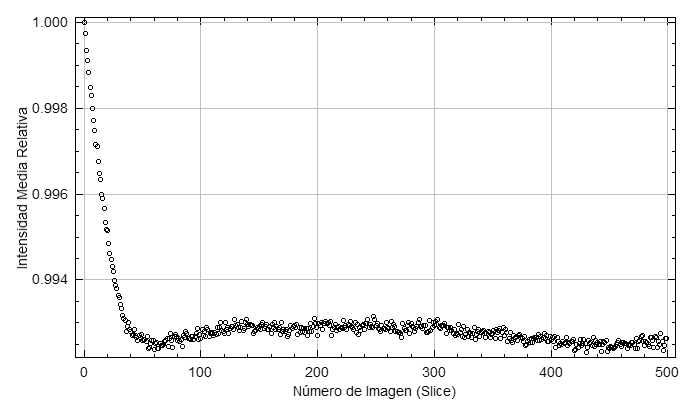
\includegraphics[width=0.8\textwidth]{images/intensidad_tiempo.png}
    \caption{Intensidad media relativa del haz de rayos X que llega al detector (a un ROI
    arbitrario de aproximadamente 100x100 pixeles), en función del número de imagen radiográfica
    adquirida para una tomografía. Se observa un máximo inicial, seguido de una rápida
    disminución y una eventual estabilización a un valor aproximado del 99.3\% del valor inicial.}
    \label{fig:intensidad_tiempo}    
\end{figure}

Para solucionar estas diferencias de la intensidad en área y tiempo, se realizan dos tipos de correcciones
distintas, presentadas a continuación. Además, la corrección en área también se encarga de la grilla hexagonal.

\subsection{Corrección de Campo Plano (FFC - Flat Field Correction)}

El objetivo de este método es corregir la intensidad del haz en función de la posición del pixel,
para un tiempo determinado, con tal de obtener uniformidad en el área. También busca corregir
posibles irregularidades en la respuesta de cada pixel, propias del detector, y la presencia del
patrón hexagonal. Para esto, además de las proyecciones radiográficas del objeto, es necesario
adquirir dos tipos de imágenes adicionales: imágenes con solo el haz incidente (sin objeto) o
\textit{flats}, e imágenes con la fuente apagada (sin haz incidente) o \textit{darks}.
Estas imágenes se adquieren con el mismo tiempo de exposición que las proyecciones radiográficas,
así como mismo voltaje y corriente de la fuente. Al mismo tiempo, es recomendable adquirir varias
imágenes de cada tipo, para luego obtener un promedio de flats y uno de darks, con el fin de reducir
el ruido.

Una vez adquiridas estas imágenes, se realiza la corrección de la intensidad $I(x,y)$ de cada pixel,
en cada proyección radiográfica, a través de la siguiente fórmula:

\begin{equation}
    I_{FFC}(x,y) = \dfrac{I(x,y) - I_{dark}(x,y)}{I_{flat}(x,y) - I_{dark}(x,y)} \times C
    \label{eq:FFC}
\end{equation}
donde $I_{dark}(x,y)$ y $I_{flat}(x,y)$ son los valores del pixel $(x,y)$ en las imágenes promedio
de darks y flats respectivamente, y $C$ es una constante de normalización que se puede elegir
arbitrariamente. En este trabajo, se definió $C$ como la moda de la intensidad (es decir, el valor
más repetido) en la imagen promedio de todas imágenes \textit{flats}. De esta forma,
se mantiene la escala de intensidad a un valor similar al que se tenía antes de la corrección.
Es importante destacar que todos los cálculos que se realizan a partir de la fórmula \ref{eq:FFC}
deben hacerse con imágenes en 32-bit, ya que en la mayoría de los casos, los valores de $I - I_{dark}$
y $I_{flat} - I_{dark}$ son muy similares, y la división entre ambos en 8 o 16 bits puede generar
errores de redondeo a 1, perdiendo la información que se busca (esto no implica que las imágenes deban
ser adquiridas en 32-bit, solamente es necesario en el cálculo).

$I_{flat}(x,y)$ contiene toda la información sobre la distribución de intensidad del haz, así como
la presencia del patrón hexagonal. Por otro lado, $I_{dark}(x,y)$ contiene información sobre el
ruido de fondo del detector, que se resta para eliminar su influencia en la corrección. De esta forma,
la fórmula \ref{eq:FFC} corrige la intensidad de cada pixel, obteniendo un haz incidente uniforme
en toda el área. 

Esta corrección es también una opción de configuración en el software del detector. Sin embargo, se encontraron dificultades
a la hora de cargar las imágenes de flats y darks en el software, por lo que para tener un mayor
control sobre el proceso, se decidió implementar la corrección de forma manual, a trevés de un
macro en FIJI (ver Apéndice B.6).

\subsection{Corrección de uniformidad temporal}

El objetivo de este método es corregir la intensidad del haz en función del tiempo (efectivamente,
número de imagen radiográfica), para obtener uniformidad temporal. Para esto, se trabaja directamente
sobre las proyecciones radiográficas, sin necesidad de aquirir imágenes adicionales.
Se considera que la intensidad relativa del haz en cada pixel, cambia aproximadamente de la misma
forma a lo largo del tiempo (es independiente de la posición del pixel). De esta forma, se corrige
cada imagen a partir de la siguiente fórmula:

\begin{equation}
    I_{T}(n,x,y) = \dfrac{I(n,x,y)}{I_{ROI}(n)} \times I_{ROI}(n_f)
    \label{eq:corr_temporal}
\end{equation}
donde $I(n,x,y)$ es la intensidad del pixel $(x,y)$ en la imagen radiográfica número $n$, $I_{ROI}(n)$
es la intensidad media en un ROI del fondo para la imagen número $n$, y $I_{ROI}(n_f)$ es la intensidad
media en el mismo ROI para la última imagen radiográfica adquirida (en la que se supone que el haz ya
se estabilizó). De esta forma, se corrige cada imagen radiográfica por su intensidad relativa,
obteniendo una serie de imágenes con una haz uniforme a lo largo del tiempo. El ROI seleccionado
debe contener solamente pixeles del fondo (sin presencia de ningún objeto), y en principio el tamaño
no es relevante, siempre y cuando se haya realizado la corrección FFC previamente a todo el set, y
esta sea satisfactoria.
Para implementar este método, se realizó un macro en FIJI (ver Apéndice B.7).

\section{Resultados} 

Se diseñaron los macros en FIJI para realizar ambas correcciones, y se aplicaron con distintos objetos
para evaluar su efectividad. En este caso, se utilizó una vértebra para adquirir proyecciones
radiográficas. Se tomaron 500 imágenes en distintas posiciones angulares (cada 0.72$^{\circ}$),
y se tomaron 5 imágenes de flats y 5 de darks para obtener los promedios. La vértebra se encuentra
en uno de los porta-muestras cilíndricos, suspendida en algodón.

En primer lugar se realizó la corrección FFC como se describió antes. Para verificar la efectividad
de esta, también se realizó sobre el conjunto de imágenes \textit{flats}. En la figura \ref{fig:res_FFC}
se observa la imagen promedio de los \textit{flats} y uno arbitrario corregido, con un mapa de color
en intensidad. En la figura \ref{fig:histogramas} se observan los histogramas de cada una de las
imágenes. Para un análisis más en detalle, se midió la intensidad media, desviación estándar y
relación señal-ruido en 154 ROIs cuadrados de 100 px de lado, distribuidos de forma equiespaciada
en toda la imagen. En la tabla \ref{tabl:FFC_flat} se encuentran los resultados. En las figuras
\ref{fig:vertebra}.a y \ref{fig:vertebra}.b se muestra una proyección arbitraria de la vértebra
y su corrección por FFC.

Por otro lado, se aplicó una transformada de Fourier rápida (FFT) al promedio de flats y a uno
de los corregidos, con el fin de estudiar la presencia de estructuras periódicas o patrones
antes y después de la corrección. Los espectros obtenidos se encuentran en la figura
\ref{fig:espectros_fourier}. Las figura \ref{fig:vertebra}.c y \ref{fig:vertebra}.d son las transformadas de Fourier
de una de una radiografías de la vertebra y su versión corregida.

\begin{figure}[htpb]
    \centering
    \begin{subfigure}{0.49\textwidth}
        \begin{overpic}[width=\linewidth]{images/Flat_Avg.png}
            \put(3, 69){\colorbox{black!60}{\color{white}\bfseries\large (a)}}
        \end{overpic}
    \end{subfigure}
    \hfill
    \begin{subfigure}{0.49\textwidth}
        \begin{overpic}[width=\linewidth]{images/flat_ffc.png}
            \put(3, 69){\colorbox{black!60}{\color{white}\bfseries\large (b)}}
        \end{overpic}
    \end{subfigure}
    \caption{Mapas de intensidad (16 bit) en el promedio de 5 imágenes \textit{flat} (\textbf{a)})
    y en uno de estos flats corregidos por \textit{flat field correcction} (\textbf{b)}).}
    \label{fig:res_FFC}    
\end{figure}

\begin{figure}[htpb]
    \centering
    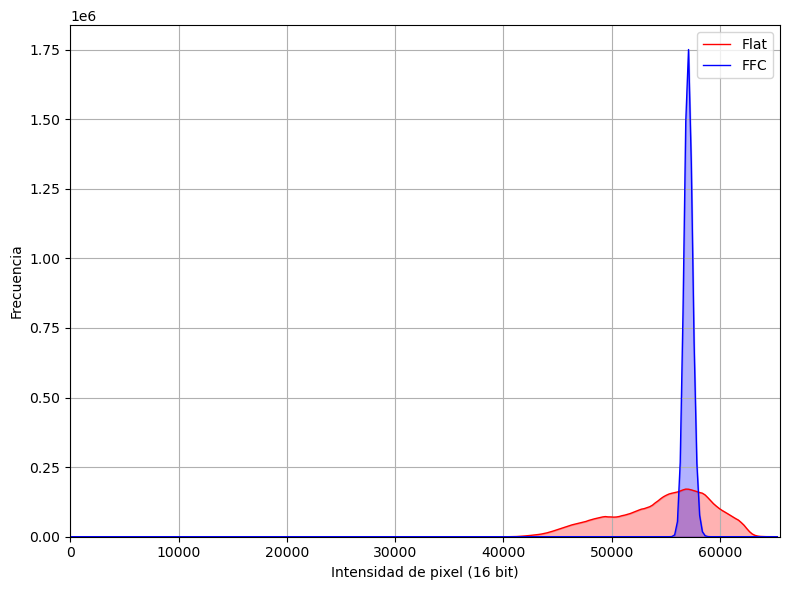
\includegraphics[width=0.55\textwidth]{images/histogramas.png}
    \caption{Histogramas correspondientes al promedio de 5 \textit{flats} (rojo), y a uno de estos
    corregido por \textit{Flat Field Correction} (azul) y normalizado con la moda de las
    intensidades del promedio de \textit{flats}.}
    \label{fig:histogramas}
\end{figure}

\begin{figure}[htpb]
    \centering
    \begin{subfigure}{0.45\textwidth}
        \begin{overpic}[width=\linewidth]{images/FFT_Flat_Avg.png}
            \put(3, 90){\colorbox{black!60}{\color{white}\bfseries\large (a)}}
        \end{overpic}
    \end{subfigure}
    \hfill
    \begin{subfigure}{0.45\textwidth}
        \begin{overpic}[width=\linewidth]{images/FFT_flat_ffc.png}
            \put(3, 90){\colorbox{black!60}{\color{white}\bfseries\large (b)}}
        \end{overpic}
    \end{subfigure}
    \caption{Espectros de Fourier del promedio de 5 imágenes \textit{flat} (\textbf{a}) y de
    uno de estos flats corregidos por \textit{flat field correction} (\textbf{b}).}
    \label{fig:espectros_fourier}    
\end{figure}

\begin{table}[htpb]
    \centering
    \caption{Promedio de parámetros estadísticos en 154 ROIs.}
    \begin{tabular}{|c|c|c|c|}
        \hline
        \textbf{Imagen} & \textbf{$VM$} & $\mathbf{\sigma}$ & \textbf{SNR} \\
        \hline
        Promedio de flats & $55100 \pm 300$ & $881 \pm 7$ & $63.0 \pm 0.5$ \\
        Flat-FFC & $57210 \pm 10$ & $367 \pm 2$ & $156.7 \pm 0.7$ \\
        \hline
    \end{tabular}
    
    \label{tabl:FFC_flat}
\end{table}

\begin{figure}[htbp]
    \centering
    % Primera fila
    \begin{overpic}[width=0.49\linewidth]{images/vertebra.png}
        \put(2, 70){\colorbox{black!50}{\color{white}\bfseries\large (a)}}
    \end{overpic}\hfill
    \begin{overpic}[width=0.49\linewidth]{images/vertebra_ffc.png}
        \put(2, 70){\colorbox{black!50}{\color{white}\bfseries\large (b)}}
    \end{overpic}
    
    \vspace{2ex} % Espaciado entre filas
    
    % Segunda fila
    \begin{overpic}[width=0.49\linewidth]{images/vertebra_fft.png}
        \put(2, 90){\colorbox{black!50}{\color{white}\bfseries\large (c)}}
    \end{overpic}\hfill
    \begin{overpic}[width=0.49\linewidth]{images/vertebra_ffc_fft.png}
        \put(2, 90){\colorbox{black!50}{\color{white}\bfseries\large (d)}}
    \end{overpic}
    
    \caption{\textbf{a)} Proyección radiográfica de una vértebra, con mapa de color de intensidad.
    \textbf{b)} Proyección radiográfica de una vértebra, corregida por \textit{flat field correction}.
    \textbf{c)} Espectro de Fourier (por FFT) de la proyección de la vértebra sin corregir (a).
    \textbf{d)} Espectro de Fourier (por FFT) de la proyección de la vértebra, corregida por
    \textit{flat field correction} (b).}
    \label{fig:vertebra}
\end{figure}

Por último, se aplicó la corrección de uniformidad temporal a las 500 imágenes corregidas por FFC,
y se observó la intensidad media en el mismo ROI del fondo para cada imagen, antes y después
de la corrección. Los resultados se encuentran en la figura \ref{fig:res_corr_temporal}.

\begin{figure}[htpb]
    \centering
    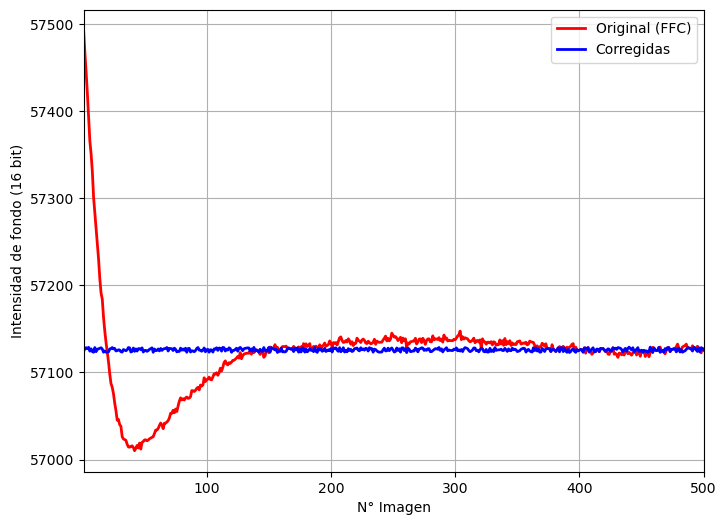
\includegraphics[width=0.8\textwidth]{images/corr_temp.png}
    \caption{Intensidad media relativa del haz de rayos X que llega al detector (a un ROI
    arbitrario del fondo), en función del número de imagen radiográfica
    adquirida para una tomografía, antes (rojo) y después (azul) de la corrección de uniformidad
    temporal.}
    \label{fig:res_corr_temporal}    
\end{figure}

\section{Discusiones}

Observando la figura \ref{fig:res_FFC}, se puede ver que la corrección FFC logra uniformizar efectivamente
la intensidad del haz en toda el área detectada. Esto mismo se puede ver en el histograma de la figura
\ref{fig:histogramas}, donde se pasa de tener un rango de intensidades de fondo entre aproximadamente
40000 y 70000 (más de 20000 niveles de intensidad), a uno mucho más reducido de entre 56000 y 58000
(menos de 2000 niveles). También la forma del histograma cambia tras la corrección, pasando de una distribución
asimétrica con dos picos distintivos (que podrían sugerir la presencia de dos ``características'' distintas,
el fondo real por un lado y el patrón hexagonal por otro), a una distribución simétrica de un solo pico,
similar a una distribución normal. Esto implica que la desviación estándar es causada principalmente por
ruido blanco, y no por otros elementos (que es lo que se desea lograr).

El histograma no es suficiente para observar la distribución espacial de la intensidad. Esto se observa
en la figura \ref{fig:res_FFC}, y con valores más concretos en la tabla \ref{tabl:FFC_flat}. La idea
de la corrección FFC es reducir la variabilidad de intensidad en cada parte del fondo, y así aumentar
la relación señal-ruido en todas las regiones por igual. Se puede ver en la tabla que esto efectivamente
sucede al aplicar la corrección. A través de esta, se logra reducir la desviación estándar, en cada ROI de
100x100 pixeles, en un factor de aproximadamente 2.4, aumentando de la misma manera el $SNR$ del fondo.
Una disminución de la desviación estándar también implica un aumento de la relación contraste-ruido, lo
que permite distinguir mejor distintas fases en una muestra. También en la figura \ref{fig:vertebra} se
observa el cambio que produce la corrección, cn mayor claridad al ver el fondo.

También a simple vista se puede notar la desaparición del patrón hexagonal en el fondo corregido.
Esto se puede observar de forma más clara y general en los espectros de Fourier de la figura
\ref{fig:espectros_fourier}. En la imagen original, se presentan una serie de picos de alta intensidad,
distribuidos en una red de Bravais triangular, correspondiente a la recíproca de una red hexagonal.
Estos picos se corresponden con los pixeles más oscuros distribuidos en una grilla hexagonal. Después
de la corrección, ningungo de estos picos permanece, lo que suguiere la desaparición por completo
de la grilla. Por otro lado, en el primer espectro de Fourier también se observan dos líneas rectas de
mayor intensidad (una vertical y otra horizontal). Estos se corresponden en primer lugar, al hecho
que la transformada de Fourier (que se define sobre un espacio infinito) se aplica al espacio finito
que es la imagen. Pero también se debe a la presencia de estructuras de filas y columnas de pixeles
con intensidades similares, propias del sistema electrónico del detector (estas son algo visibles
en la imagen de la figura \ref{fig:res_FFC}.a). Al restar la imagen \textit{Dark} durante la corrección,
estas estructuras desaparacen, lo que en el espectro de Fourier se observa como una disminución
drástica de estas dos líneas rectas.

En una radiografía de una muestra típica (un hueso por ejemplo), no suele haber componenetes de alta
frecuencia, esto es, no suele haber muchos cambios de fase en una sección muy pequeña (del orden de un
pixel), por lo que las componentes propias de la muestra se encuentran contenidas en el centro de 
de la imagen de la transformada, la cual no es afectada por estos cambios. Esto se observa con
mayor claridad al estudiar la figura \ref{fig:vertebra}. A pesar de que la imagen de la vértebra
sea mucho más ``compleja'' que un fondo blanco como el de la figura \ref{fig:res_FFC}, sus espectros
de Fourier no son muy distintos, ya que los picos más intensos se encuentran en el centro de la imagen
(frecuencias bajas), mientras que el patrón hexagonal y las líneas horizontales y verticales se distinguen
fácilmente del resto. Al aplicar la corrección FFC, son estos últimos componentes los que desaparecen
o se atenúan drásticamente, mientras que el efecto en el centro es menor.

Finalmente, se observa la efectividad de la corrección temporal de la intensidad en la figura
\ref{fig:res_corr_temporal}. El resultado es una intensidad constante, más un ruido blanco
propio del sistema. De esta forma, las proyecciones presentan uniformidad del fondo en área
y tiempo, permitiendo una reconstrucción más fiel de los valores de gris de voxel. Además,
estos resultados son fundamentales para poder realizar mediciones reales a partir de los
niveles de grises, como el coeficiente de atenuación o la densidad en un mismo material, ya
que permiten obtener valores consistentes para distintas tomografías (siempre y cuando los
parámetros de voltaje y corriente de la fuente sean los mismos). Este es un paso esencial
para poder determinar una calibración del nivel de gris en una tomografía.
\chapter{Consideraciones finales y conclusiones}
\label{conclusiones}

A lo largo del trabajo se han realizado varias reconstrucciones tomográficas de distintos
objetos, para verificar visualmente la efectividad de la alineación en situaciones reales.

\section{Algunas reconstrucciones tomográficas}

Las siguientes son imágenes obtenidas a partir de reconstrucciones tomográficas, adquiridas con
el microtomógrafo. La figura \ref{fig:reloj_rec} presenta dos cortes tomográficos del mecanismo
de un reloj reconstruidos a partir de una misma adquisición (mismos parámetros). Sin embargo, se utilizaron distintos
parámetros en la reconstrucción, alineados en una y desalineados en la otra, diferencia que se
observa claramente por los artefactos de ``doble imagen'' en la fig. \ref{fig:reloj_rec}.b. Esto
demuestra la importancia de la correcta alineación y calibración geométrica, incluso si las
correcciones parecen ``pequeñas''. La figura \ref{fig:reloj3d} es la reconstrucción tridimensional
correspondiente a la fig. \ref{fig:reloj_rec}.a, y se observa una muy buena definición de las
formas geométricas y volúmenes de las piezas mecánicas. Algunas partes parecen más ``difuminadas'',
a causa de ser componentes con superficie amplia pero muy delgados.

Por otro lado, en las figuras \ref{fig:hueso_rec} y \ref{fig:vertebra_rec} se observan reconstrucciones
de muestras biológicas, con formas orgánicas y no tan definidas como las piezas mecánicas de un
reloj. Aún así, se observa un alto nivel de detalle, y se se llegan a apreciar características de
las muestras (como cavidades) de tamaños de hasta 50 $\mu$m. En la figura \ref{fig:hueso_rec}.b
parece haber artefactos de líneas rectas, sobre todo en las zonas más densas del hueso, causadas
por el ``re-slicing'' que se hizo a partir de los cortes transversales de \ref{fig:hueso_rec}.a.
Sin embargo, no parece haber otros artefactos. La figura \ref{fig:vertebra_rec} por otro lado,
aunque también presenta una muy buena resolución espacial, parece tener más artefactos de intensidad,
como puntos y líneas más brillantes, o un ``ruido'' alrededor de la vértebra, debido a la presencia
de elementos de alta densidad en ciertas regiones.

Finalmente, la figura \ref{fig:mandibulas} muestra dos cortes transversales de mandíbulas de rata (muestras distintas, pero comparables),
reconstruidos a partir de una reconstrucción con un microtomógrafo Bruker y con el de arquitectura
abierta, y adquiridas con los mismos parámetros. Aunque los cortes no son de la misma muestra, se observa que en cuestión
de calidad de imagen, nivel de detalle, reconstrucción de las formas y resolución espacial, ambas
reconstrucciones son comparables, y prácticamente imposible de determinar el origen de cada una.

\begin{figure}[htpb]
    \centering
    \begin{subfigure}{0.49\textwidth}
        \begin{overpic}[width=\linewidth]{images/reloj_rec.png}
            \put(3, 90){\colorbox{black!60}{\color{white}\bfseries\large (a)}}
        \end{overpic}
    \end{subfigure}
    \hfill
    \begin{subfigure}{0.49\textwidth}
        \begin{overpic}[width=\linewidth]{images/reloj_rec1.png}
            \put(3, 90){\colorbox{black!60}{\color{white}\bfseries\large (b)}}
        \end{overpic}
    \end{subfigure}
    \caption{Cortes tomográficos reconstruidos del mecanismo de un reloj, a partir de parámetros corregidos
    (\textbf{a}) y a partir de un sistema desalineado (\textbf{b}). En la segunda, se observa una
    ``superposición'' de imágenes, con una leve diferencia angular, causada por la desalineación. Parámetros
    de adquisición: 90 kV (Voltaje), 47 $\mu$A (Corriente), 1200 proyecciones, $M=2.55$ y resolución de pixel
    de 24.4 $\mu$m.}
    \label{fig:reloj_rec}    
\end{figure}

\begin{figure}[htpb]
    \centering
    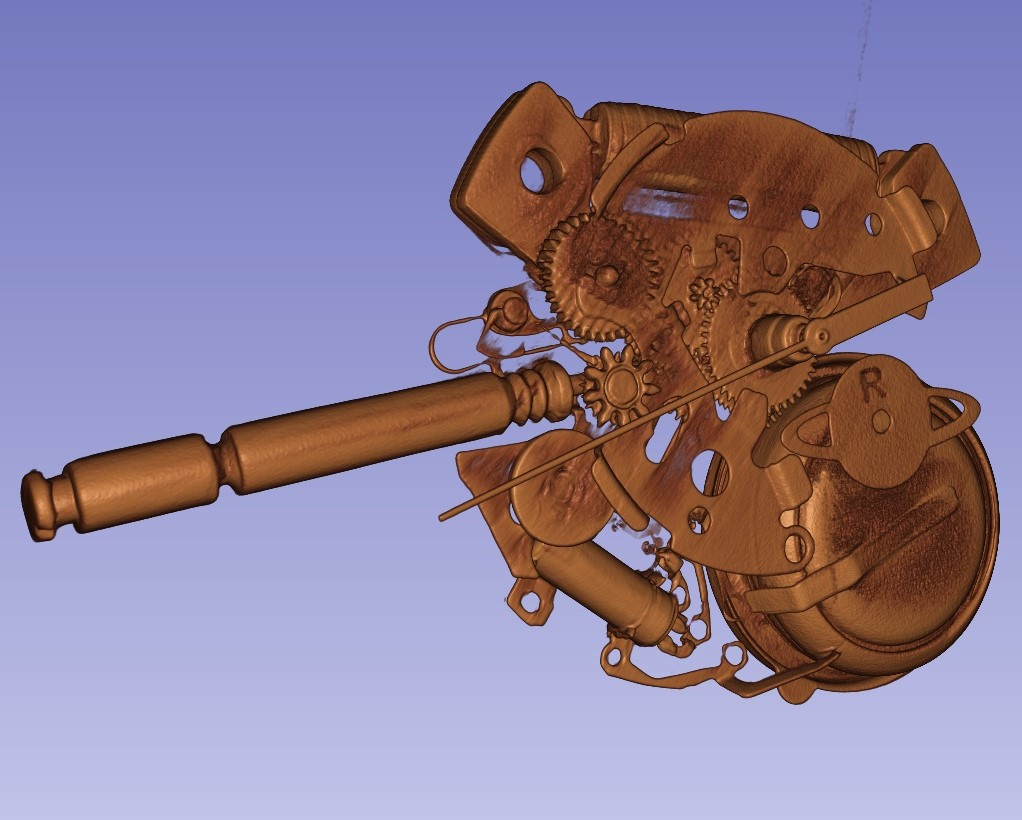
\includegraphics[width=0.65\textwidth]{images/reloj3d.jpg}
    \caption{Visión tridimensional de la reconstrucción tomográfica del mecanismo de un reloj
    (utilizando el software 3DSlicer).}
    \label{fig:reloj3d}
\end{figure}

\begin{figure}[htpb]
    \centering
    \begin{subfigure}{0.26\textwidth}
        \begin{overpic}[width=\linewidth]{images/hueso_rec1.png}
            \put(1, 88){\colorbox{black!60}{\color{white}\bfseries\large (a)}}
        \end{overpic}
    \end{subfigure}
    \hfill
    \begin{subfigure}{0.73\textwidth}
        \begin{overpic}[width=\linewidth]{images/hueso_rec2.png}
            \put(0.5, 31.5){\colorbox{black!60}{\color{white}\bfseries\large (b)}}
        \end{overpic}
    \end{subfigure}
    \caption{Reconstrucción tomográfica de un hueso (fémur) de rata. \textbf{a)} Corte tomográfico
    axial, donde se pueden observar cavidades de hasta 50 $\mu$m de diámetro. \textbf{b)} Corte
    tomográfico sagital (rotado 90$^{\circ}$) del hueso. Se observan diferencias de densidad en distintas
    regiones del hueso, dadas por las diferencias de intensidad. Parámetros de adqusición: 90 kV (voltaje),
    47 $\mu$A (corriente), 1200 proyecciones, $M=2.06$ y resolución de pixel de 24.3 $\mu$m.}
    \label{fig:hueso_rec}    
\end{figure}

\begin{figure}[htpb]
    \centering
    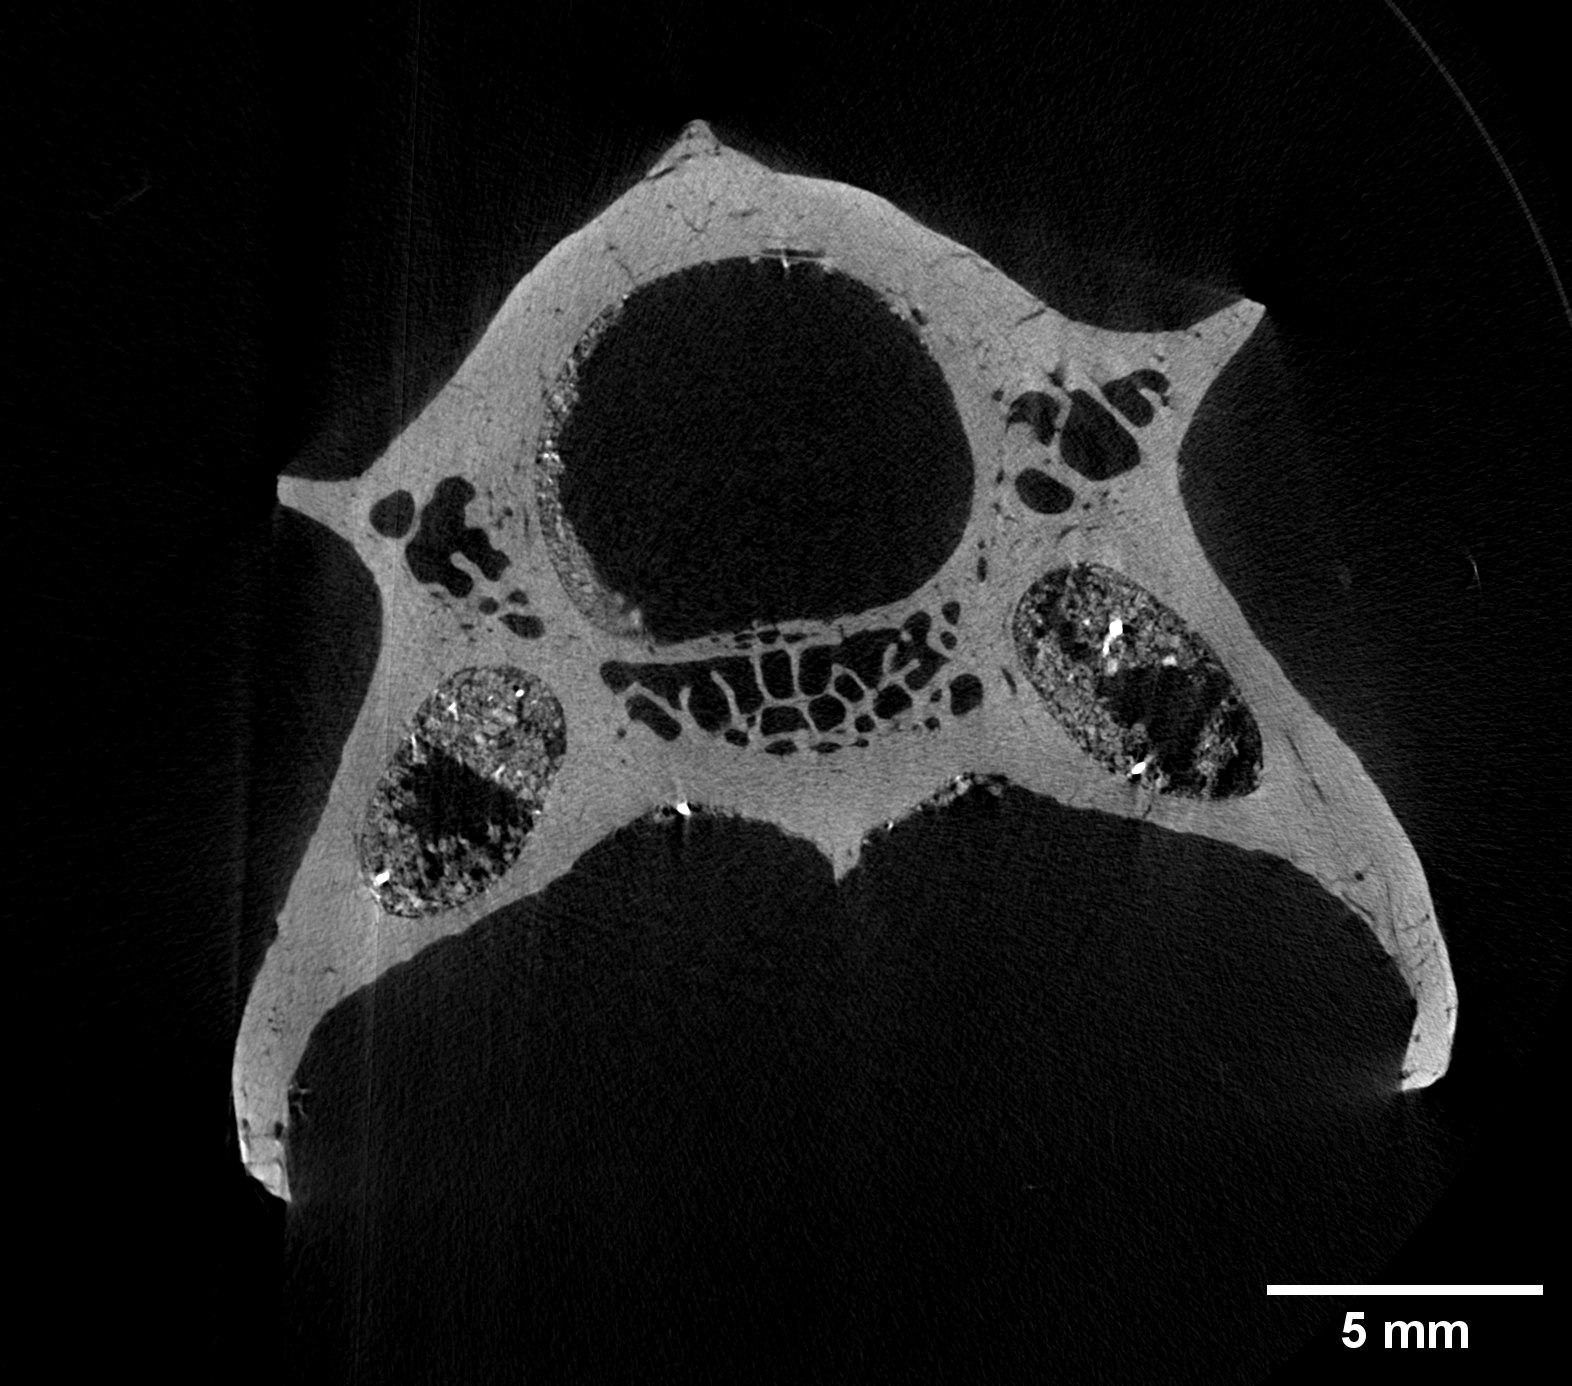
\includegraphics[width=0.5\textwidth]{images/verte_rec_0.png}
    \caption{Corte tomográfico axial reconstruido de una vértebra, correspondiente a las proyecciones
    de la figura \ref{fig:vertebra}.}
    \label{fig:vertebra_rec}
\end{figure}

\begin{figure}[htpb]
    \centering
    \begin{subfigure}{0.40\textwidth}
        \begin{overpic}[width=\linewidth]{images/mandibula_BK.png}
            \put(3, 90){\colorbox{black!60}{\color{white}\bfseries\large (a)}}
        \end{overpic}
    \end{subfigure}
    \hspace{7mm}
    \begin{subfigure}{0.40\textwidth}
        \begin{overpic}[width=\linewidth]{images/mandibula_AA.png}
            \put(3, 90){\colorbox{black!60}{\color{white}\bfseries\large (b)}}
        \end{overpic}
    \end{subfigure}
    \caption{Cortes transversales reconstruidos de dos mandíbulas de rata similares. (\textbf{a})
    Reconstrucción a partir de una adquisición con un microtomógrafo marca Bruker. (\textbf{b})
    Reconstrucción a partir de una adquisición con el microtomógrafo de arquitectura abierta
    trabajado. Parámetros de adquisición: 70 kV (Voltaje), 142 $\mu$A (Corriente), 471 proyecciones,
    $M=1.44$, resolución de pixel de 25.0 $\mu$m.}
    \label{fig:mandibulas}    
\end{figure}

\newpage

\section{Conclusiones}

A partir del desarrollo experimental y el análisis de resultados presentados en este trabajo,
se pueden extraer las siguientes conclusiones generales en relación con los objetivos planteados
inicialmente:

Se cumplió satisfactoriamente con la optimización
del microtomógrafo de arquitectura abierta del laboratorio LAMARX. La transición hacia un
diseño con fuente y detector fijados sobre una base rígida fue un paso crítico que permitió
minimizar las desalineaciones accidentales y garantizó la estabilidad necesaria para procesos
de adquisición prolongados.

La alineación física inicial, mediante el análisis de círculos proyectados y la
superposición de cilindros reflejados, demostró ser un método robusto para reducir las
desviaciones angulares fuera de plano ($\theta$ y $\phi$) a valores menores a 5$^{\circ}$, y para
aproximar el punto principal del eje de magnificación al centro del detector. No
obstante, se concluye que este proceso tiene una alta dependencia de la destreza del
operador y de particularidades mecánicas del sistema.

En cuanto a la calibración analítica, el método de múltiples proyecciones y análisis de trayectorias
elípticas resultó
ser una herramienta altamente confiable y consistente para determinar parámetros finos como
la distancia fuente-detector $D$, la distancia fuente-objeto $F$, la posición del punto principal $\mathcal{P}$,
y la inclinación de los ejes en el plano del detector ($\eta$).
Por el contrario, el método de una única proyección se reveló
como inconsistente e impráctico para las condiciones del laboratorio, debido a su extrema
sensibilidad a la posición del fantoma y a la amplificación de errores en sus
complejas operaciones matemáticas.

Se logró caracterizar eficazmente la resolución espacial del sistema a partir del análisis de
la función de transferencia de modulación ($MTF$), obtenida del análisis de bordes. Se determinó
que para este sistema, se tiene una resolución espacial de entre 15 y 60
$\mu$m, en el rango de magnificaciones posibles del detector ($M<7$). Se concluye que las aproximaciones
teóricas estándar de la resolución subestiman este valor, lo que validó la necesidad de introducir una
corrección empírica (parámetro $c$) para modelar adecuadamente el comportamiento del equipo.
Asimismo, se verificó que el método de la lámina inclinada es un sustituto rápido y equivalente
a la medición sobre reconstrucciones tomográficas para caracterizar la MTF.

La implementación manual de técnicas de
pre-procesamiento fue determinante para la calidad de los resultados finales. La Corrección
de Campo Plano (FFC) no solo uniformizó la intensidad del haz, sino que eliminó con éxito el
patrón hexagonal del detector y las estructuras electrónicas de ruido, logrando aumentar la
relación señal-ruido (SNR) en un factor de 2.4. Adicionalmente, la corrección temporal compensó
eficazmente la inestabilidad de la fuente de rayos X, asegurando una reconstrucción libre
de artefactos de intensidad.

La efectividad de todo el protocolo desarrollado
fue validada visualmente mediante la reconstrucción de objetos complejos. La obtención de
imágenes nítidas en muestras biológicas (fémur de rata, mandíbula y vértebra) y mecánicas, con la
capacidad de distinguir microestructuras (del tamaño esperado según los cálculos de resolución
espacial), confirma que el sistema se encuentra
calibrado para realizar investigación científica de alta precisión, compitiendo con un
microtomógrafo comercial de alto nivel. A su vez, se probó la
repetibilidad del protocolo, al ser utilizado más de una vez, en configuraciones distintas del
sistema.

En conclusión, este trabajo establece un protocolo de calibración sistemático y reproducible,
transformando un conjunto de componentes independientes en un instrumento de microtomografía
funcional y preciso, capaz de competir con soluciones comerciales en términos de calidad de imagen,
flexibilidad y trazabilidad de datos.

\subsection{Perspectivas a futuro}

La naturaleza de ``arquitectura abierta'' del microtomógrafo implica un potencial inmenso de
mejoras y modificaciones, todas en función del tipo de uso que se requiera del mismo.

En primer lugar, y continuando con las ideas presentadas en el capítulo \ref{cap:cal_intensidad},
es de interés diseñar un método de calibración del nivel de gris, para lograr mediciones reales
y consistentes del coeficiente de atenuación lineal de una muestra, utilizando materiales de
referencia o nuevos fantomas.

Por otro lado, se puede seguir avanzando sobre la estructura física del mismo. Algunas ideas
ya se han nombrado a lo largo del trabajo, como mejorar la base de soporte y el sistema de rieles, acoplar
el porta-muestra a esta misma base (y tener un sistema totalmente acoplado), mejorar los sistemas de
fijación de las muestras, añadir más micro-motores,
y por lo tanto, grados de libertad de movimiento controlado a cada componente, entre otros.

También sería posible realizar avances en el software del equipo, ya sea para añadir otros componentes
como micro-motores, o para el procesamiento y análisis de las proyecciones radiográficas y tomografías.
En este trabajo, se demostró la utilidad de herramientas como FIJI, capaces de implementar macros y
plugins que automatizan procesos complejos, pero solo se observó una pequeña fracción de su potencial.
Por otro lado, la corrección de algunos artefactos, como el endurecimiento del haz, son posibles de tratar
solamente con softwares especializados.

En este campo y por último, es importante destacar el gran avance
que han tenido los modelos de Machine Learning y Redes Neuronales para el tratamiento de imágenes,
no solo en la identificación y corrección de errores y artefactos, sino también en la
segmentación avanzada y automatizada. 


\appendix
% Redefine el formato de capítulo a una sola línea para los apéndices
\titleformat{\chapter}[hang]
  {\normalfont\huge\bfseries}
  {\chaptertitlename\ \thechapter:}
  {15pt}
  {\Huge}

\label{apendice_A}

\chapter{Método de calibración de una proyección}

\section*{Ecuaciones y fórmulas del método}

A continuación se describen las fórmulas y ecuaciones utilizadas en el método de calibración
de una única proyección (\ref{cap:cal_espacial}). En el artículo de Sun et al. \cite{Sun2006}
se explican con mayor detalle.

\subsection*{1. Resolución de ángulos principales}

La ecuación para hallar el ángulo $\phi$ se plantea de forma implícita, igualando la relación de distancias observadas con la expresión teórica:

\begin{equation}
\frac{L_{13}}{L_{24}} = \frac{2F - l\cdot \tan(\phi)}{2F + l\cdot \tan(\phi)}
\end{equation}

De manera análoga, la ecuación implícita para obtener el ángulo auxiliar $\Gamma$ es:

\begin{equation}
\frac{L_{12}}{L_{34}} = \frac{\sqrt{l^2 + 4F^2} - l\cdot \tan(\Gamma)}{\sqrt{l^2 + 4F^2} + l\cdot \tan(\Gamma)}
\end{equation}

\subsection*{2. Ángulos auxiliares}

Los ángulos $\alpha$ y $\beta$ se definen a partir de los parámetros geométricos del sistema:

\begin{align}
\alpha &= \arctan\left(\frac{l}{\sqrt{l^2 + 4F^2}}\right) \\
\beta &= \arctan\left(\frac{l}{2F}\right)
\end{align}

\subsection*{3. Cálculos geométricos}

Las longitudes de los segmentos espaciales $SI$, $ES$, $EI$, $OI$ y $OE$ se calculan en secuencia:

\begin{align}
SI &= \frac{D \sqrt{\left(\frac{l}{2F}\right)^2 + 1}}{1 + \left(\frac{l}{2F}\right) \tan(\phi)} \\
ES &= \frac{SI \cos(\Gamma)}{\cos(\alpha - \Gamma)} \\
EI &= \sqrt{ES^2 + SI^2 - 2 \cdot ES \cdot SI \cos(\alpha)} \\
OI &= \frac{l \cdot D}{2F \cos(\phi) + l \sin(\phi)} \\
OE &= \sqrt{ES^2 + D^2 - 2 \cdot ES \cdot D \cos(\alpha) \cos(\beta)}
\end{align}

\subsection*{4. Ángulos espaciales adicionales}

El coseno del ángulo $\gamma$ se obtiene aplicando el teorema del coseno generalizado, para luego calcular el ángulo $\theta$:

\begin{align}
\cos(\gamma) &= \sqrt{1 - \left(\frac{OI^2 + EI^2 - OE^2}{2 \cdot OI \cdot EI}\right)^2} \\
\theta &= \arccos\left(\frac{\cos(\Gamma)}{\cos(\gamma)}\right)
\end{align}

\subsection*{5. Cálculo de la corrección $z$}

La variable $z$ se obtiene resolviendo la siguiente ecuación implícita:

\begin{equation}
L_{13} = \frac{(D + z) \sqrt{\left(\frac{l}{F}\right)^2 + 4} \cos(\Gamma) \sin(2\alpha)}{\left(2 + \frac{l}{F} \tan(\phi)\right) \cos(\alpha + \Gamma) \cos(\alpha - \Gamma)}
\end{equation}

\subsection*{6. Parámetros del plano auxiliar y transformación de coordenadas}

Dado un punto inicial con coordenadas $(u, v)$, se calcula el punto de intersección $(u_t, v_t)$ en el plano auxiliar:

\begin{align}
u_t &= -\frac{OI}{2} + \frac{EI^2 - OE^2}{2 \cdot OI} \\
v_t &= \sqrt{EI^2 - (OI + u_t)^2}
\end{align}

A partir de estas coordenadas, se determina el ángulo de rotación $\eta$:

\begin{equation}
\eta = \arcsin\left(\frac{2(u \cdot v_t - v \cdot u_t)}{u_t^2 + v_t^2}\right)
\end{equation}

Las desviaciones $du$ y $dv$ se calculan aplicando una matriz de rotación:

\begin{align}
dU &= (u - u_t)\cos(\eta) - (v - v_t)\sin(\eta) \\
dV &= (u - u_t)\sin(\eta) + (v - v_t)\cos(\eta)
\end{align}

\subsection*{7. Corrección focal y aumento}

Finalmente, se calcula la corrección de la distancia focal $\Delta F$:

\begin{align}
\Delta F &= \frac{F \cdot z}{D + z} \\
\end{align}


\chapter{Macros para FIJI}
\section*{Macros diseñados para FIJI}

A continuación se presentan los códigos utilizados.

\vspace{1em} % Añade un pequeño espacio antes del bloque
\captionof{listing}{Macro de FIJI para el análisis de la proyección del cono de RX.}
\label{cod:proyeccion_cono}
\inputminted[linenos, breaklines, frame=lines, fontsize=\footnotesize]{java}{macros/proyeccion_cono.ijm}
\vspace{1em} % Añade un pequeño espacio después del bloque

\vspace{1em} % Añade un pequeño espacio antes del bloque
\captionof{listing}{Macro de FIJI para el análisis de un objeto cilíndrico y su reflejo rotado.}
\label{cod:analisis_cilindro}
\inputminted[linenos, breaklines, frame=lines, fontsize=\footnotesize]{java}{macros/analisis_cilindro.ijm}
\vspace{1em} % Añade un pequeño espacio después del bloque

\vspace{1em} % Añade un pequeño espacio antes del bloque
\captionof{listing}{Macro de FIJI para la obtención de centroides de esferas en trayectoria elíptica.}
\label{cod:centroides_esferas}
\inputminted[linenos, breaklines, frame=lines, fontsize=\footnotesize]{java}{macros/centroides_esferas.ijm}
\vspace{1em} % Añade un pequeño espacio después del bloque

\vspace{1em} % Añade un pequeño espacio antes del bloque
\captionof{listing}{Macro de FIJI para la medición de múltiples perfiles de intensidad perpendiculares a una línea.}
\label{cod:perfiles}
\inputminted[linenos, breaklines, frame=lines, fontsize=\footnotesize]{java}{macros/perfiles.ijm}
\vspace{1em} % Añade un pequeño espacio después del bloque

\vspace{1em}
\captionof{listing}{Macro de FIJI para la generación de cortes radiales mediante detección automática del eje central.}
\label{cod:cortes_radiales}
\inputminted[linenos, breaklines, frame=lines, fontsize=\footnotesize]{java}{macros/cortes_radiales.ijm}
\vspace{1em}

\vspace{1em}
\captionof{listing}{Macro de FIJI para la corrección de campo plano (FFC) en proyecciones microtomográficas.}
\label{cod:ffc}
\inputminted[linenos, breaklines, frame=lines, fontsize=\footnotesize]{java}{macros/FFC.ijm}
\vspace{1em}

\vspace{1em}
\captionof{listing}{Macro de FIJI para la corrección temporal de la uniformidad de haz.}
\label{cod:correccion_temporal}
\inputminted[linenos, breaklines, frame=lines, fontsize=\footnotesize]{java}{macros/correccion_temporal.ijm}
\vspace{1em}

\cleardoublepage % Asegura que el enlace apunte a la página correcta
\addcontentsline{toc}{chapter}{\bibname} % \bibname imprime "Bibliografía"
\bibliographystyle{babunsrt}
\bibliography{bibliografia}

\end{document}
